\ifx\allfiles\undefined
\documentclass[8pt a4paper, oneside, UTF8]{ctexbook} 
\usepackage{amsmath}   % 数学公式
\usepackage[dvipsnames]{xcolor}
\usepackage{amsthm}    % 定理环境
\usepackage{amssymb}   % 更多公式符号
\usepackage{graphicx}  % 插图
\usepackage{mathrsfs}  % 数学字体
\usepackage{enumitem}  % 列表
\usepackage{geometry}  % 页面调整
\usepackage{unicode-math}
\usepackage{extarrows}
\usepackage{subfigure}
\usepackage{extarrows}
\usepackage{footnote}
\usepackage{svg}
\usepackage[colorlinks,linkcolor=black]{hyperref}
\usepackage{supertabular}
\usepackage{tcolorbox}
\usepackage{ulem}
\usepackage{framed}
\usepackage{float}
\usepackage{microtype}
\newcommand{\arccot}{\mathrm{arccot}\,}
\tcbuselibrary{breakable}
\tcbuselibrary{most}
\newcounter{problemname}
\newenvironment{solution}{\par\noindent\textbf{解答. }}{\par}
\newenvironment{note}{\par\noindent\textbf{题目\arabic{problemname}的注记. }}{\par}
\definecolor{shadecolor}{RGB}{241, 241, 255}
\newenvironment{problem}{\begin{shaded}\stepcounter{problemname}\par\noindent\textbf{题目\arabic{problemname}. }}{\end{shaded}\par}

\graphicspath{ {figure/},{../figure/}, {config/}, {../config/} }  % 配置图形文件检索目录
\linespread{1.2} % 行高

% 页码设置
\geometry{top=25.4mm,bottom=25.4mm,left=20mm,right=20mm,headheight=2.17cm,headsep=4mm,footskip=12mm}

% 设置列表环境的上下间距
\setenumerate[1]{itemsep=5pt,partopsep=0pt,parsep=\parskip,topsep=5pt}
\setitemize[1]{itemsep=5pt,partopsep=0pt,parsep=\parskip,topsep=5pt}
\setdescription{itemsep=5pt,partopsep=0pt,parsep=\parskip,topsep=5pt}

% 定理环境
% ########## 定理环境 start ####################################

% #### 将 config.tex 中的定理环境的对应部分替换为如下内容
% 定义单独编号,其他四个共用一个编号计数 这里只列举了五种,其他可类似定义(未定义的使用原来的也可)
\newtcbtheorem[auto counter, number within=section, list type=subsubsection, list inside=toc]{defn}{定义}
{
    colback=green!5,colframe=green!35!black,fonttitle=\bfseries, title={Comment \thetcbcounter}, list entry={Comment \thetcbcounter\quad}, %标题
    breakable, %支持跨页
    before upper={\parindent10pt\noindent},  % 支持缩进。\noindent:首行不缩进
    % left = 2mm, %文字离线框左边的边距
    % right = 1mm,%同上
    % top = 1mm,%同上
    % bottom = 1mm,%同上
    % arc is angular = 1mm, % 棱角线框
    % sharp corners, % 直角线框
    % enhanced,frame hidden, % 隐藏线框
    % enhanced, drop fuzzy shadow,  % 显示阴影
}
{def}

\newtcbtheorem[auto counter, number within=section, list type=subsubsection, list inside=toc]{lemma}{引理}
{
    colback=SeaGreen!10!CornflowerBlue!10,colframe=RoyalPurple!55!Aquamarine!100!,fonttitle=\bfseries, title={Comment \thetcbcounter}, list entry={Comment \thetcbcounter\quad}, %标题
    breakable, %支持跨页
    before upper={\parindent10pt\noindent},  % 支持缩进。\noindent:首行不缩进
    % left = 2mm, %文字离线框左边的边距
    % right = 1mm,%同上
    % top = 1mm,%同上
    % bottom = 1mm,%同上
    % arc is angular = 1mm, % 棱角线框
    % sharp corners, % 直角线框
    % enhanced,frame hidden, % 隐藏线框
    % enhanced, drop fuzzy shadow,  % 显示阴影
}
{lem}


\newtcbtheorem[auto counter, number within=section, list type=subsubsection, list inside=toc]{them}{定理}
{
    colback=Salmon!20, colframe=Salmon!90!Black,fonttitle=\bfseries, title={Comment \thetcbcounter}, list entry={Comment \thetcbcounter\quad}, %标题
    breakable, %支持跨页
    before upper={\parindent10pt\noindent},  % 支持缩进。\noindent:首行不缩进
    % left = 2mm, %文字离线框左边的边距
    % right = 1mm,%同上
    % top = 1mm,%同上
    % bottom = 1mm,%同上
    % arc is angular = 1mm, % 棱角线框
    % sharp corners, % 直角线框
    % enhanced,frame hidden, % 隐藏线框
    % enhanced, drop fuzzy shadow,  % 显示阴影
}
{them}
\newtcbtheorem[auto counter, number within=section, list type=subsubsection, list inside=toc]{criterion}{注}
{
    colback=CornflowerBlue!10,colframe=RoyalPurple!55!Aquamarine!100!,fonttitle=\bfseries, title={Comment \thetcbcounter}, list entry={Comment \thetcbcounter\quad}, %标题
    breakable, %支持跨页
    before upper={\parindent10pt\noindent},  % 支持缩进。\noindent:首行不缩进
    % left = 2mm, %文字离线框左边的边距
    % right = 1mm,%同上
    % top = 1mm,%同上
    % bottom = 1mm,%同上
    % arc is angular = 1mm, % 棱角线框
    % sharp corners, % 直角线框
    % enhanced,frame hidden, % 隐藏线框
    % enhanced, drop fuzzy shadow,  % 显示阴影
}
{cri}

\newtcbtheorem[auto counter, number within=section, list type=subsubsection, list inside=toc]{corollary}{推论}
{
    colback=Emerald!10,colframe=cyan!40!black,fonttitle=\bfseries, title={Comment \thetcbcounter}, list entry={Comment \thetcbcounter\quad}, %标题
    breakable, %支持跨页
    before upper={\parindent10pt\noindent},  % 支持缩进。\noindent:首行不缩进
    % left = 2mm, %文字离线框左边的边距
    % right = 1mm,%同上
    % top = 1mm,%同上
    % bottom = 1mm,%同上
    % arc is angular = 1mm, % 棱角线框
    % sharp corners, % 直角线框
    % enhanced,frame hidden, % 隐藏线框
    % enhanced, drop fuzzy shadow,  % 显示阴影
}
{cor}
% colback=red!5,colframe=red!75!black

% ######### 定理环境 end  #####################################

% ↓↓↓↓↓↓↓↓↓↓↓↓↓↓↓↓↓ 以下是自定义的命令  ↓↓↓↓↓↓↓↓↓↓↓↓↓↓↓↓

% 用于调整表格的高度  使用 \hline\xrowht{25pt}
\newcommand{\xrowht}[2][0]{\addstackgap[.5\dimexpr#2\relax]{\vphantom{#1}}}

% 表格环境内长内容换行  
\newcommand{\tabincell}[2]{\begin{tabular}{@{}#1@{}}#2\end{tabular}}

% 使用\linespread{1.5} 之后 cases 环境的行高也会改变,重新定义一个 ca 环境可以自动控制 cases 环境行高
\newenvironment{ca}[1][1]{\linespread{#1} \selectfont \begin{cases}}{\end{cases}}
% 和上面一样
\newenvironment{vx}[1][1]{\linespread{#1} \selectfont \begin{vmatrix}}{\end{vmatrix}}

\def\d{\textup{d}} % 直立体 d 用于微分符号 dx
\def\R{\mathbb{R}} % 实数域
\newcommand{\bs}[1]{\boldsymbol{#1}}    % 加粗,常用于向量
\newcommand{\ora}[1]{\overrightarrow{#1}} % 向量

% 数学 平行 符号
\newcommand{\pll}{\kern 0.5em/\kern -0.8em /\kern 0.5em}

% 用于空行\myspace{1} 表示空一行 填 2 表示空两行  
\newcommand{\myspace}[1]{\par\vspace{#1\baselineskip}}

\begin{document}
\begin{sloppypar}
    % \title{{\Huge{\textbf{高等数学笔记}}}}
\author{作者:于家崇}
\date{\today}
\maketitle                   % 在单独的标题页上生成一个标题

\thispagestyle{empty}        % 前言页面不使用页码
\begin{center}
	\Huge\textbf{前言}
\end{center}

If a job is worth doing,it's worth doing well
\begin{flushright}
	\begin{tabular}{c}
		\today \\ 如果一件事值得去做,那就值得去做好
	\end{tabular}
\end{flushright}

\newpage                      % 新的一页
\pagestyle{plain}             % 设置页眉和页脚的排版方式(plain:页眉是空的,页脚只包含一个居中的页码)
\setcounter{page}{1}          % 重新定义页码从第一页开始
\pagenumbering{Roman}         % 使用大写的罗马数字作为页码
\tableofcontents              % 生成目录

\newpage                      % 以下是正文
\pagestyle{plain}
\setcounter{page}{1}          % 使用阿拉伯数字作为页码
\pagenumbering{arabic}
% \setcounter{chapter}{-1}    % 设置 -1 可作为第零章绪论从第零章开始 
    \else
    \fi
    %  ############################ 正文部分
    \chapter{极限}
    \section{数列的极限}
    \subsection{数列极限的定义}
    \begin{defn}{数列极限的定义}{}
        设$|x_n|$为一数列,若\uwave{存在常数$a$},对于\uwave{任意的$\varepsilon>0$(不论它多么小)},\uwave{总存在正整数$N$},使得当\uwave{$n>N$}时 \uwave{$|x_n-a|<\varepsilon$ 恒成立},则称数 $a$是数列$| x_n |$的极限,或者称数列$| x_n |$收敛于 $a$,记为
        $$
            \lim_{n\to\infty}x_n=a\text{或}x_n\to a(n\to\infty)
        $$
        该定义的$\varepsilon-N$\footnote{$\varepsilon - N$\textcolor{red}{几何意义: 对于点$a$的任何$\varepsilon$邻域即开区间$(a-\varepsilon,a+\varepsilon)$一定存在$N$,当$n < N$即第$N$项以后的点$x_n$都落在开区间$(a-\varepsilon,a+\varepsilon)$内,而只有有限个(最多有$N$个)在区间之外.}}语言描述是
        $$\lim_{n\to\infty}x_n=a\Leftrightarrow\forall\varepsilon>0,\exists\text{正整数}N,\text{当}n>N\text{时},\text{有}|x_n,-a|<\varepsilon.$$
    \end{defn}
    在上面的定义中,$\varepsilon>0$的$\varepsilon$任意性是非常重要的,只有这样才能表示出\textcolor{red}{无限接近的意义}.总存在正整数$N$,使得$n>N$这个条件用于表达$n \to \infty$的过程.
    \begin{criterion}{数列极限的性质}{}
        \begin{itemize}
            \item 数列收敛\footnote{区别于级数收敛}等价于数列极限存在
            \item \textcolor{red}{数列的极限值与数列的前有限列无关,只与后面无穷项有关}
            \item \textcolor{red}{数列的最值只能在前有限项中取得,前有限项有比极限值大的,则数列存在最大值.前有限项有比极限值小的,则数列存在最小值}
            \item \textcolor{red}{若数列$\{a_n\}$收敛,则其任何子列$\{a_{n_k}\}$也收敛,且$\lim_{k\to\infty}a_{n_k}=\lim_{n\to\infty}a_n$}\footnote{ 此条定理提供了一个判断数列发散的方法:1.至少一个子数列发散.2.两个子数列收敛,但是收敛值不同.}
            \item $\underset{n\to\infty}{\operatorname*{\lim}}x_n=a\Leftrightarrow\underset{k\to\infty}{\operatorname*{\lim}}x_{2k-1}=\underset{k\to\infty}{\operatorname*{\lim}}x_{2k}=a$
        \end{itemize}
    \end{criterion}
    \begin{conclusion}{数列极限常用结论}{}
        \begin{itemize}
            \item \textbf{$\lim_{n \to \infty }\sqrt[n]{n}=1.\lim_{n \to \infty} \sqrt[n]{a}=1(a>0)$}\label{jl1}
            \item 关于数列$(1+\dfrac{1}{n})^n$的结论
            \begin{itemize}
                \item 单调增加
                \item $\lim_{n\to \infty}(1+\dfrac{1}{n})^n=e$
            \end{itemize}
        \end{itemize}
    \end{conclusion}
    \begin{problem}
        已知$a_{n}=\sqrt[n]{n}-\dfrac{(-1)^{n}}{n}(n=1,2,\cdots)$,则${a_n}$\\
        (A) 有最大值,有最小值 \quad (B) 有最大值,没有最小值 \\ (C)没有最大值,有最小值 \quad (D)没有最大值,没有最小值
    \end{problem}
    \begin{solution}
        $\lim_{n\to \infty}a_n=1-0$,$a_1=2,a_2=\sqrt{2}-\dfrac{1}{2}$,因此$a_n$既有最大值又有最小值
    \end{solution}
    \begin{problem}
        证明:\textcolor{red}{若$\lim_{n \to \infty}a_n=A$,则$\lim_{n \to \infty}|a_n|=|A|$}
    \end{problem}
    \begin{proof}
        已知数列$a_n$极限为$A$,那么$|a_n-A|<\varepsilon$,由不等式\ref{lyzybds1}可得,$||a_n|-|A||\leqslant|a_n -A|<\varepsilon$,因此$\lim_{n \to \infty }|a_n|=|A|$.
        \end{proof}
    \begin{corollary}{上题题目推论}{}
        \begin{enumerate}
            \item 此命题反过来则错误,如取$a_n=(-1)^n$,则$\lim_{n\to\infty}\left|(-1)^n\right|=1$.但$\lim_{n\to\infty}(-1)^n$不存在.
            \item 在本题中若$A=0$,则$||a_n|-|A||=||a_n|-0|=|a_n-0|$,即有
            $$
            \lim_{n\to\infty}a_{n}=0\Leftrightarrow\lim_{n\to\infty}\lvert a_{n}\rvert=0\:,
            $$
            此结论常用,即若要证明$\lim _{n \to \infty}a_n=0$,可转换为证明$\lim_{n \to \infty}|a_n|=0$,由于$|a_n| \geq 0$,若使用了夹逼准则,只需证明$|a_n|\leqslant 0$即可
            \item 此结论对函数亦成立,即\textcolor{red}{若$\lim_{x\to x_0 }f\left(x\right)=A$,则$\lim_{x\to x_0}\left|f\left(x\right)\right|=\left|A\right|.$}
        \end{enumerate}
    \end{corollary}
    \begin{problem}
        设$\lim_{n \to +\infty} a_n=a$,且$a\neq0$,则当$n$ 充分大时有\\
        $\mathrm{(A)}\mid a_n\mid>\dfrac{\mid a\mid}{2}.\quad\mathrm{(B)}\mid a_n\mid<\dfrac{\mid a\mid}{2}.\quad\mathrm{(C)}a_n>a-\dfrac{1}{n}.\quad\mathrm{(D)}a_n<a+\dfrac{1}{n}.$
    \end{problem}
    \begin{solution}
        根据结论若$\lim_{x\to x_0 }f\left(x\right)=A$,则$\lim_{x\to x_0}\left|f\left(x\right)\right|=\left|A\right|.$可得$\lim_{n \to \infty}a_n=a \Rightarrow \lim_{n \to \infty}|a_n|=|a|$,即$|a_n|>|a| > \dfrac{|a|}{2}$.
    \end{solution}
    \begin{note}
        对于C,D选项,只知道$a_n$的极限是$a$,那么就是说两者之间的距离是无穷小,但是题目中没有给出两者相距的量级,因此一定错误的.反例为$a_n= a \pm \dfrac{1}{n^2}$.\label{pro3}
    \end{note} 
    \begin{problem}
        设数列${x_n} $与${y_n}$满足$\lim_{n \to \infty} x_ny_n=0$,则下列命题正确的是\\
        (A)若$x_n$发散,则$y_n$,必发散\quad (B)若$x_n$无界,则 $y_n$必有界\\
        (C)若$x_n$有界,则 $y_n$必为无穷小 \quad(D)若$\dfrac{1}{x_n}$为无穷小,则$y_{n}$必为无穷小
    \end{problem}
    \begin{solution}
        A选项:令$x_n=\begin{cases}
            0, n\text{为奇数}\\
            n, n\text{为偶数}
        \end{cases}$,$y_n \equiv 0$.显然$x_n$发散,但是$y_n$收敛.\\
        B选项:令$x_n=\begin{cases}
            0, n\text{为奇数}\\
            n, n\text{为偶数}
        \end{cases}$,$y_n=\begin{cases}
            n, n\text{为偶数}\\
            0, n\text{为奇数}
        \end{cases}$.虽然二者都无界,但是也满足题意.\\
        C选项:令$x_n \equiv 0$,$y_n=\begin{cases}
            n, n\text{为奇数}\\
            0, n\text{为偶数}
        \end{cases}$.同理也满足题意,但是$y_n$为无穷大\\
        D选项:$\lim_{n \to \infty}x_n y_n=\lim_{n \to \infty} \dfrac{y_n}{\frac{1}{x_n}}=0 \Rightarrow y_n=o(\dfrac{1}{x_n})$
    \end{solution}
    \begin{note}
        数列极限概念题一个很好的办法是\textcolor{red}{举反例.经典反例:(1)分奇偶.(2)恒为0.}
    \end{note}
    \begin{problem}
        设$x_n$与${y_n}$为两个数列,则下列说法正确的是\\
        (A)若$ x_n$与${y_n}$无界,则{$ x_n+y_n$}无界\\
        (B)若$x_n$ 与${y_n}$无界,则{$x_ny_n$}无界\\
        (C)若${x_n}$ 与${y_n}$ 中,一个有界,一个无界,则{$x_ny_n$}无界\\
        (D)若$x_n$ 与$ y_n$ 均为无穷大,则$ x_ny_n$ 一定为无穷大
    \end{problem}
    \begin{solution}
        A选项:令$a_n=n$,$b_n=-n$,显然$x_n$,$y_n$无界,但是$x_n+y_n$有界\\
        B选项:令$x_n=\begin{cases}
            0, n\text{为奇数}\\
            n,n\text{为偶数}
        \end{cases}$,$y_n=\begin{cases}
            n,n\text{为奇数}\\
            0, n\text{为偶数}
        \end{cases}$,显然$x_n,y_n$无界,但是$x_n y_n$有界\\
        C选项:令$x_n=\begin{cases}
            0, n\text{为奇数}\\
            n,n\text{为偶数}
        \end{cases}$,$y_n \equiv 0$,显然$x_n$一个有界,一个无界,但是二者相乘为有界\\
        D选项:无穷大$\times$无穷大=无穷大
    \end{solution}
    \begin{problem}
        设$x_n$与${y_n}$为两个数列,则下列说法正确的是\\
        (A)若$\lim_{n\to\infty} x_ny_n=0$,则必有$\lim_{n\to\infty} x_n=0$ 或$\lim_{n\to\infty} y_n=0$\\
        (B)若$\lim_{n\to\infty} x_ny_n=\infty$,则必有$\lim_{n\to\infty} x_n=\infty$ 或$\lim_{n\to\infty}y_n=\infty$\\
        (C)若 $x_ny_n$ 有界,则必有 $x_n$ 与 $y_n$ 都有界.\\
        (D)若 $x_ny_n$ 无界,则必有 $x_n$ 无界或 $y_n$ 无界
    \end{problem}
    \begin{solution}
        A选项:令$x_n=\begin{cases}
            0, n\text{为奇数}\\
            n,n\text{为偶数}
        \end{cases}$,$y_n=\begin{cases}
            n,n\text{为奇数}\\
            0, n\text{为偶数}
        \end{cases}$,显然$x_n \cdot y_n \equiv 0$,但是$x_n y_n$两者都无界.\\
        B选项: 令$x_n=\begin{cases}
            1,n\text{为奇数}\\
            n,n\text{为偶数}
        \end{cases}$,$y_n=\begin{cases}
            n,n\text{为奇数}\\            
            1,n\text{为偶数}
        \end{cases}$,显然二者相乘为$\infty$,但是二者都是无界,没有极限\\
        C选项:同A选项\\
        D选项:使用逆否命题:若$x_n$有界且$y_n$有界,则$x_n \cdot y_n$有界,显然成立,有界$\times$ 有界=有界
    \end{solution}
    \begin{note}
       \textcolor{red}{在证明中,使用逆否命题可以减少复杂度},如本题的D选项.
    \end{note}
    \begin{problem}
        设$\lim_{n\to\infty} a_n$ 与$\lim_{n\to\infty} b_n$ 均不存在,则下列选项正确的是\\
        A.若$\lim_{n \to \infty}(a_n+b_n$)不存在,则$\lim_{n \to \infty}(a_n-b_n)$ 必不存在 \\ 
        B.若$\lim_{n \to \infty}(a_n+b_n$)不存在,则$\lim_{n \to \infty}(a_n-b_n$)必存在\\
        C.若$\lim_{n \to \infty}(a_n+b_n$)存在,则$\lim_{n \to \infty}(a_n-b_n)$ 必不存在 \\ 
        D.若$\lim_{n \to \infty}(a_n+b_n$)存在,则$\lim(a_n-b_n)$ 必存在
    \end{problem}
    \begin{solution}
        A选项:$a_n=e^n,b_n=e^n$,显然$\lim_{n \to \infty}(a_n+b_n)$不存在,但是$\lim_{n \to \infty}(a_n-b_n)$存在\\
        B选项:$a_n=e^n,b_n=2e^{n}$,显然$\lim_{n \to \infty}(a_n+b_n)$不存在,但是$\lim_{n \to \infty}(a_n-b_n)$也不存在\\
        C选项:若$\lim_{n \to \infty}(a_n+b_n)$存在,假设$\lim_{ n \to \infty}(a_n-b_n)$存在,那么$\lim_{n\to \infty}[(a_n+b_n)-(a_n-b_n)]$也应该存在,但是$\lim_{n \to \infty}=2 b_n$,根据题意可知不存在,因此假设错误\\
        D选项:$a_n=e^n,b_n=-e^n$,显然$\lim_{n \to \infty}(a_n+b_n)$存在,但是$\lim_{n \to \infty}(a_n-b_n)$不存在
    \end{solution}

    \subsection{收敛数列的性质}
    \subsubsection{唯一性}
    \begin{defn}{数列极限唯一性的定义}{}
        如果数列$\{ x_n \}$收敛,那么它的极限唯一
    \end{defn}
    \subsubsection{有界性}
    \begin{defn}{数列收敛的有界性的定义}{}
        如果数列$\{x_n\}$收敛,那么数列$\{x_n\}$一定有界\footnote{如果数列有界,但是不一定存在极限,如数列$(-1)^n$}.
    \end{defn}
    \subsubsection{保号性}
    \begin{defn}{数列极限保号性的定义}{}
        如果$\lim_{n\to\infty}x_n=a$,且$a{>}b( $或 $a{<}b)$,那么存在正整数 $N$,当 $n{>}N$ 时 ,都有$x_n{>}b($ 或 $x_n{<}b$.\newline
        如果数列$\mid x_n\mid$从某项起有$x_n\geqslant b($或$x_n\leqslant b)$,且$\lim_{n\to\infty}x_n=a $,那么 $a\geqslant b( 或 a\leqslant b)$\footnote{其中b可以为任意实数,常考b=0的情况}.
    \end{defn}
    \begin{problem}
        下列结论中错误的是\\
        (A)设$\lim _{n\to\infty}a_n=a>1$,则存在$M>1$,当$n$ 充分大时,有$a_n>M$\\
        (B)设$a=\lim_{n\to\infty}a_n<\lim_{n\to\infty}b_n=b$,则当$n$ 充分大时,有$a_n<b_n$ \\
        (C)设$M\leqslant a_n\leqslant N(n=1,2,...)$,若$\lim_{n\to\infty} a_n=a$,则$M\leqslant a\leqslant N$ \\
        (D)若$\lim_{n\to\infty} a_n=a\neq0$,则当$n$充分大时,$a_n>a-\dfrac1n$ 
    \end{problem}
    \begin{solution}
        A选项:若$\lim_{n \to \infty}a_n=a$,那么当$n$充分大时,$a_n$的值趋近于$a$,那么肯定存在一个$M$,满足$a_n = a \geqslant M > 1.$\\
        B选项:若 $a_n$ 的极限$>b_n$ 的极限,则当$n$ 充分大时,$a_n>b_n$.\\
        C选项:不等式左右取极限可得C选项正确\\
        D选项:题目3解析\ref{pro3}出有解释,同理
    \end{solution}
    \begin{note}
        数列极限的保号性可写为:\textcolor{red}{两个数列 $a_n$ 和 $b_n$,若 $a_i>b_i$ 恒成立,且$\lim_{n \to \infty}a_n$和$\lim_{n\to \infty}b_n$都存在.则 $n$ 趋于无穷时,$a_n$的极限$\geqslant b_n$ 的极限.(对不等式取极限时,$>$要变成$\geqslant$,<要变成$\leqslant,\geqslant$不用变,$\leqslant$不用变).}\\
        \textcolor{red}{若 $a_n$ 的极限$>b_n$ 的极限,则当$n$ 充分大时,$a_n>b_n$.}\footnote{证明如下:令$x_n=b_n-a_n$,则$\lim_{n \to \infty}x_n=\lim_{n\to \infty}(b_n-a_n)=b-a>0$.由极限的保号性可知,当$n$充分大的时候,$x_n>0$,即$b_n>a_n$}\\
        \textcolor{red}{若 $a_n$ 的极限$\geqslant b_n$ 的极限,则当$n$充分大时,$a_n$和$b_n$大小无法确定.}
    \end{note}

    \section{函数的极限}
    \subsection{超实数系}
    \begin{defn}{超实数系的概念}{}
        超实数(Hyperreal number)是一个包含实数以及无穷大和无穷小的域,它们的绝对值分别大于和小于任何正实数.
    \end{defn}
    \begin{criterion}{超实数集}{}
        \begin{itemize}
            \item 超实数集\textcolor{red}{是为了严格处理无穷量(无穷大量和无穷小量)而提出的}.
            \item 超实数集,或称为非标准实数集,记为$^{*}\mathbb{R}$,是实数集$\mathbb{R}$的一个扩张.
        \end{itemize}
    \end{criterion}
    \subsection{邻域}\footnote{邻域与区间不同,邻域属于区间的范畴.但是邻域通常表示“一个局部位置”.比如“点$x_0$的$\delta$”邻域,可以理解为“点$x_0$”的附近,而区间是明确指出在实数系下的范围}
    \begin{defn}{邻域的相关概念}{}
        \begin{itemize}
            \item $\delta$邻域:设$x_0$是数轴上一个点,$\delta$是某一正数,则称$(x_{0}-\delta,x_{0}+\delta)$为点$x_0$的$\delta$邻域,记作$U(x_{0},\delta)$,即:
                  $$
                      U(x_{0},\delta)=\left\{x|x_{0}-\delta<x<x_{0}+\delta\right\}=\left\{\left.x\right|\left|\left.x-x_{0}\right|<\delta\right\}\right.
                  $$
            \item 去心$\delta$邻域:定义点$x_0$的去心邻域$\mathring{U}(x_{0},\delta)=\bigl\{x|0<\bigl|x-x_{0}\bigr|<\delta\bigr\}$
            \item 左,右$\delta$邻域:$\left\{x|0<x-x_{0}<\delta\right\}$称为点$x_0$的右$\delta$邻域,记作$U^{+}(x_{0},\delta);\{x|0<x_{0}-x<\delta\}$称为点$x_0$的左$\delta$邻域,记作$U^{-}(x_{0},\delta).$
        \end{itemize}
    \end{defn}
    \subsection{函数极限的定义}
    函数极限的定义主要分为自变量趋于有限值$(x \to x_0)$时的极限和自变量趋于无穷大时函数的极限$(x \to \infty)$
    \subsubsection{自变量趋于有限值时的函数极限}
    \begin{defn}{当自变量趋于有限值时函数极限定义}{}
        设函数$f(x)$在点$x_0$的某一去心邻域内有定义.如果存在常数$A$,对于任意给定的正数$\varepsilon$\textcolor{red}{(不论它多么小)\footnote{$\varepsilon$用于衡量$|f(x)-A|$的值有多小}},总存在正数$\delta$,使得当$x$满足不等式$0<|x-x_0|<\delta$时,对应的函数值$f(x)$都满足不等式
        $$
            |f(x)-A|<\varepsilon
        $$
        那么常数$A$就叫做\uwave{函数$f(x)$当$x \to x_0$时的极限},记作:
        $$
            \lim_{x\to x_0}f(x)=A\quad\text{或}f(x)\to A(\text{当}x\to x_0)
        $$
        其$\varepsilon-N$语言为
        $$
            \lim_{x\to x_0}f(x)=A\Leftrightarrow\forall\varepsilon>0,\exists\delta>0,\text{当}0<|x-x_0|<\delta\text{时},\text{有}|f(x)-A|<\varepsilon.
        $$
        $\forall\varepsilon>0,\exists\delta>0$在证明中,这两句是白给,直接写.后面的才是关键.
    \end{defn}
    \begin{criterion}{函数极限注意事项}{}
        \begin{enumerate}
            \item 在函数极限中$x \to \infty$指的是$|x| \to \infty$,需要$x$趋于正无穷和负无穷,但在数列中的$n \to \infty$是$n \to +\infty$
            \item \textcolor{red}{函数的极限值只与邻域内的函数值有关,而与该点的函数值无关}.
        \end{enumerate}
    \end{criterion}
    \begin{problem}
        设$\lim_{x \to 1}\dfrac{f(x)}{\ln x}=1$,则:\\
        $(A) f(1)=0 \quad (B)\lim_{x\to 1}f(x)=0 \quad (C)f'(1)=1 \quad (D)\lim_{x \to 1}f'(x)=1$
    \end{problem}
    \begin{solution}
        $\lim_{x\to 1}\ln x=0$,根据极限四则运算法则\ref{jxdsz1},$\lim_{x \to 1} f(x)=0$,对于其他选项,需要知道的是函数的极限值与该点的函数值无关,只与邻域内的函数值有关.
    \end{solution}
    \subsubsection{单侧极限}
    \begin{defn}{单侧极限的定义}{}
        若当$x\to x_0^{-}$时,$f(x)$无限接近于某常数$A$,则常数$A$叫作函数$f(x)$当$x\to x_0$时的\textcolor{red}{左极限},记为
        \begin{center}
            $\operatorname*{lim}_{x\to x_0^{-}}f(x)=A$或 $f(x_0^{-})=A$.
        \end{center}
        若当$x\to x_0^+$时,$f(x)$无限接近于某常数$A$,则常数$A$叫作函数$f(x)$当$x\to x_0$时的\textcolor{red}{右极限},记为
        \begin{center}
            $\operatorname*{lim}_{x\to x_0^{+}}f(x)=A$或 $f(x_0^{+})=A$
        \end{center}
    \end{defn}
    \begin{problem}
    $\text{已知}\lim_{x\to0}\biggl[a\arctan\dfrac{1}{x}+(1+\mid x\mid)^{\frac{1}{x}}\biggr]\text{存在,求}a\text{的值}$
    \end{problem}
    \begin{solution}
        由于存在$\arctan$与$|x|$函数,则对于0点的极限值需要分左右进行计算.

        $\lim\limits_{x\to0^{-}}\left[\begin{matrix}a\arctan\dfrac{1}{x}+(1+\mid x\mid)^{\frac{1}{x}}\\\end{matrix}\right]=\lim\limits_{x\to0^{-}}a\arctan\dfrac{1}{x}+\lim\limits_{x\to0^{-}}(1-x)^{\frac{1}{x}}=-\dfrac{\pi}{2}a+\dfrac{1}{\text{e}}$

        $\lim\limits_{x\to0^+}\left[\begin{matrix}a\arctan\dfrac{1}{x}+(1+\mid x\mid)^{\frac{1}{x}}\\\end{matrix}\right]=\lim\limits_{x\to0^+}a\arctan\dfrac{1}{x}+\lim\limits_{x\to0^+}(1+x)^{\frac{1}{x}}=\dfrac{\pi}{2}a+\mathrm{e}$
        若极限存在,则$a=\dfrac{1-e^2}{\pi e}$
    \end{solution}
    \begin{note}
        由于自变量趋向的双向性,以下类型的函数因此需要进行特殊讨论:
        \begin{itemize}
            \item 形如$f(x)=max\{h(x),g(x)\}$此类函数也需要注意在函数变化点的自变量取值问题
            \item $\lim_{x \to \infty}e^x$:$\lim _{x \to +\infty}e^x=+\infty,
                      \lim _{x \to -\infty}e^x=0$
            \item $\lim_{x \to 0} \dfrac{\sin x}{|x|}$:$\lim_{x \to 0^+}=\dfrac{\sin x}{x}=1$,$\lim_{x \to 0^-}=\dfrac{\sin x}{-x}=-1$
            \item $\lim_{x \to \infty }\arctan x$:$\lim_{x \to +\infty}\arctan x=\dfrac{\pi}{2}$,$\lim_{x \to -\infty}\arctan x= -\dfrac{\pi}{2}$
            \item $\lim_{x \to 0}[x]$:$\lim _{x \to 0^+}[x]=0,\lim_{x \to 0^-}[x]=-1$
        \end{itemize}
    \end{note}
    \subsubsection{自变量趋于无穷大时函数的极限}
    \begin{defn}{自变量趋于无穷大时函数极限定义}{}
        设函数$f(x)$在点$x_0$的某一去心邻域内有定义.如果存在常数$A$,对于任意给定的正数$\varepsilon$.(不论它多么小),总存在正数$\delta$,使得当$x$满足不等式$0<|x-x_0|<\delta$时,对应的函数值$f(x)$都满足不等式
        $$
            |f(x)-A|<\varepsilon
        $$
        那么常数$A$叫做函数$f(x)$当$x \to x_0$的极限,记作:
        $$
            \lim_{x\to x_0}f(x)=A\text{或}f(x)\to A(\text{当}x\to x_0)
        $$
        其$\varepsilon-N$语言为
        $$
            \lim\limits_{x\to x_0}f(x)=A\Leftrightarrow\forall\varepsilon>0,\exists\delta>0,\text{当}0<|x-x_0|<\delta\text{时},\text{有}|f(x)-A|<\varepsilon.
        $$
        $\forall\varepsilon>0,\exists\delta>0$在证明中,这两句是白给,直接写.后面的才是关键.
    \end{defn}
    \textcolor{red}{需要注意的是趋向的值不同时,$\varepsilon -N$写法不同,不能照抄}.其$\varepsilon -N$的表达为如下表格:
    \begin{center}
        \begin{tabular}{|c|c|c|c|c|}
            \hline
            & \textcolor{red}{$f(x)\to A$} & \textcolor{red}{$f(x)\to \infty$} & \textcolor{red}{$f(x)\to +\infty$} & \textcolor{red}{$f(x)\to -\infty$}\\
            \hline
            $x \to x_0$       & $\begin{aligned}&\forall\varepsilon>0,\exists\delta>0, \\&\text{使当 }0<\mid x-x_0\mid  \\&<\delta\text{ 时 },\text{即有} \\&|f(x)-A|<\varepsilon.\end{aligned}$ & $\begin{aligned}&\forall M>0,\exists\delta>0, \\&\text{使当 }0<\mid x-x_{0}\mid  \\&<\delta\text{ 时 },\text{即有}\\& |f(x)|>M\end{aligned}$ & $\begin{aligned}&\forall M>0,\exists\delta>0, \\&\text{使当} 0<|x-x_0| \\ &<\delta \text{时 ,即有} \\ &f(x)>M.\end{aligned}$      & $\begin{aligned}&\forall M>0,\exists\delta>0, \\&\text{使当 }0<\mid x-x_{0}\mid  \\&<\delta\text{ 时 ,即有}\\& f(x) <-M\end{aligned}$ \\ \hline
            $x \to x_0^+$     & $\begin{aligned}&\forall\varepsilon>0,\exists\delta>0, \\&\text{使当 }0<x-x_{0}< \\&\delta \text{时,即有}\\&|f(x)-A|<\varepsilon.\end{aligned}$                  & $\begin{aligned}&\forall M>0,\exists\delta>0, \\&\text{使当 }0<x-x_{0}< \\&\delta \text{时,即有} \\&|f(x)|>M.\end{aligned}$                  & $\begin{aligned}&\forall M>0,\exists\delta>0, \\&\text{使当 }0<x-x_{0}< \\&\delta \text{时,即有} \\&f(x)>M.\end{aligned}$         & $\begin{aligned}&\forall M>0,\exists\delta>0, \\&\text{使当 }0<x-x_{0}<\delta  \\&\text{时,即有} \\& f(x) <-M\end{aligned} $          \\ \hline
            $x \to x_0^-$     & $\begin{aligned}&\forall\varepsilon>0,\exists\delta>0, \\&\text{使当}0>x-x_{0}> \\&-\delta\text{ 时 },\text{即有} \\&|f(x)-A|<\varepsilon.\end{aligned}$         & $\begin{aligned}&\forall M>0,\exists\delta>0, \\&\text{使当 }0>x-x_{0}> \\&-\delta\text{ 时 },\text{即有} \\&|f(x)|>M.\end{aligned}$         & $\begin{aligned}&\forall M>0,\exists\delta>0, \\&\text{使当}0>x-x_{0}> \\&-\delta\text{ 时 },\text{即有}\\& f(x) >M\end{aligned}$ & $\begin{aligned}&\forall M>0,\exists\delta>0, \\&\text{使当 }0>x-x_{0}> \\&-\delta\text{ 时 },\text{即有}\\&f(x) <-M\end{aligned}$    \\ \hline
            $x\to \infty$     & $\begin{aligned}&\forall\varepsilon>0,\exists X>0, \\&\text{使当}\mid x\mid>X\text{ 时 }, \\&\text{即有} \\&|f(x)-A|<\varepsilon.\end{aligned}$                  & $\begin{aligned}&\forall M>0,\exists X>0,\\& \text{使当}\mid x\mid>X \\&\text{时,即有}\\&|f(x)|>M\end{aligned}$                              & $\begin{aligned}&\forall M>0,\exists X>0, \\&\text{使当}\mid x\mid>X \\&\text{时,即有}\\& f(x)>M\end{aligned}$                    & $\begin{aligned}&\forall M>0,\exists X>0, \\&\text{使当|x|>X时,} \\&\text{即有} \\&f(x)<-M.\end{aligned}$                             \\ \hline
            $x \to + \infty $ & $\begin{aligned}&\forall\varepsilon>0,\exists X>0, \\&\text{使当x>X时,} \\&\text{即有} \\&|f(x)-A|<\varepsilon.\end{aligned} $                                   & $\begin{aligned}&\forall M>0,\exists X>0, \\&\text{使当 }x>X\text{ 时 }, \\&\text{即有}\\& |f(x)|>M\end{aligned}$                            & $\begin{aligned}&\forall M>0,\exists X>0,\\&\text{使当}x>X\text{时},\\&\text{即有}\\&f(x)>M.\end{aligned}$                        & $\begin{aligned}&\forall M>0,\exists X>0, \\&\text{使当x>X时,} \\&\text{即有}\\&f(x)<-M\end{aligned}$                                 \\ \hline
            $x \to -\infty$   & $\begin{aligned}&\forall\varepsilon>0,\exists X>0, \\&\text{使当}x<-X\text{ 时 }, \\&\text{即有} \\&|f(x)-A|<\varepsilon.\end{aligned}$                          & $\begin{aligned} & \forall M>0 , \exists X> 0,\\&\text{使当 }x<-X \\&\text{时,即有}\\&|f(x)|>M\end{aligned}$                                 & $\begin{aligned} &\forall M>0,\exists X> 0,\\&\text{使当 }x<-X \\&\text{时,即有}\\&f(x)>M\end{aligned}$                           & $\begin{aligned}&\forall M>0,\exists X>0,\text{使}\\&\text{当}x<-X\text{时},\text{即有}\\&f(x)< -M.\end{aligned}$                     \\ \hline
        \end{tabular}
    \end{center}
    \begin{criterion}{上表的部分解释}{}
        \begin{itemize}
            \item 以$\lim_{x \to x_0}f(x)=A$为例:不管$f(x)$与$A$的距离多近($\forall \varepsilon >0$),总有$x$不断靠近$x_0$,使得$|f(x)-A|<\varepsilon$.
            \item 以$\lim_{x\to \infty}f(x)=\infty$为例:不管$M$多大,总有当$x>\infty$时,使得$|f(x)>M|$,即满足$\lim_{x\to \infty}f(x)=\infty$.
        \end{itemize}
    \end{criterion}
    \subsection{函数极限的性质}
    \subsubsection{唯一性}
    \begin{them}{}{}
        如果$\lim\limits_{x\to x_0}f(x)$存在,那么极限唯一
    \end{them}
    \begin{criterion}{关于唯一性的说明}{}
        \begin{itemize}
            \item 对于$x \to \infty$,意味着$x \to +\infty$且$x \to -\infty$
            \item 对于$x \to x_0$,意味着$x \to x_0^+$且$x \to x_0^-$
                  \newline
                  对于上述问题,我们称为自变量取值的“双向性”.以下有一些常见的问题:
                  \begin{itemize}{}{}
                      \item $\lim_{x\to \infty} e^x$ 不存在, $\lim_{x \to 0}\dfrac{\sin x}{|x|}$不存在, $\lim_{x\to \infty} \arctan x$不存在, $\lim_{x\to x_0} [x]$不存在.
                      \item 其不存在的原因均为分段函数分段点极限表达式不同,需要分别求左右极限.
                  \end{itemize}
        \end{itemize}
    \end{criterion}
    \begin{criterion}{极限存在的充要条件}{}
        $$
            \lim_{x\to x_0}f(x)=A\Leftrightarrow\lim_{x\to x_0^-}f(x)=A,\text{且}\lim_{x\to x_0^+}f(x)=A\footnote{左右极限都存在且相等}
        $$
        $$
            \lim_{x\to x_0}f(x)=A\Leftrightarrow f(x)=A+\alpha(x),\lim_{x\to x_0}\alpha(x)=0(\text{无穷小量}\alpha(x)=0)\footnote{对于此概念,如果引入超实数系的解释应为$A$是$f(x)$的标准实数部分,而$f(x)$的值是超实数系下的值,因此其值应为$f(x)=A+\alpha(x)$}
        $$
    \end{criterion}
    \begin{criterion}{极限不存在的情况}{}
        \begin{itemize}
            \item \textcolor{red}{函数在该点附近趋于无穷}
            \item 函数在该点的左右极限只存在一个,或两者都存在但不相等
            \item 函数在该点附近不停地震荡
            \item 该点是函数无定义点的聚点
        \end{itemize}
    \end{criterion}
    
    \subsubsection{局部有界性}
    \begin{them}{}{}
        若极限$\lim_{x \to x_0}f(x)$存在\footnote{对局部有界性的描述需要指明是在那个区间上},则$f(x)$在点$x_0$某去心邻域内有界.
    \end{them}
    \begin{criterion}{局部有界性的性质}{}
        \begin{itemize}
            \item 极限存在必有界,有界函数极限不一定存在.
            \item 若$y=f(x)$在$[a,b]$上为连续函数,则$f(x)$在$[a,b]$上必有界.
            \item \textcolor{red}{若$f(x)$在$(a,b)$内为连续函数,且$\lim_{x \to a^+}f(x)$与$\lim_{x\to b^-}f(x)$都存在,则$f(x)$在$(a,b)$内必定有界.}
            \item 有界函数与有界函数的和,差,积仍为有界函数\footnote{商不是有界函数,因为:$y_1=1,y_2=0,\dfrac{y_1}{y_2}=\infty$}.
        \end{itemize}
    \end{criterion}
    \begin{problem}
    在下列区间内,函数$f(x)={\dfrac{x\sin(x-3)}{(x-1)(x-3)^{2}}}$有界的是:\\
    A:(-2,1) \qquad  B:(-1,0)\qquad C:(1,2) \qquad D:(2,3)
    \end{problem}
    \begin{solution}
        又题意可知,函数的分段点为$x=3,0,1$,对上述三点求极限,分析可得,当$x=3,1$时,函数极限为$\infty$,因此函数在上述两点的极限不存在,因此根据局部有界性的性质可得,含这两个点的区间无界,因此排除A,C,D.答案为B.
    \end{solution}
    \subsubsection{局部保号性}
    \begin{them}{}{}
        如果$\lim_{x\to x_0}f(x)=A$,且$A>0$(或$A<0$),那么存在常数$\delta>0$,使得当$0<|x-x_0|<\delta$时有$f(x)>0(或f(x)<0)$\footnote{如果函数在$x_0$附近的极限值为正,那么$x_0$附近的函数值为正}.
        \\
        如果在$x_0$的某去心邻域内$f(x)\geqslant 0$(或$f(x)\leqslant 0$),而且$\underset{x\to x_0}{\operatorname*{lim}}f(x)=A$,那么$A \leqslant 0$或$(A \leq 0)$\footnote{如果函数在$x_0$附近的函数值$\leq 0$,那么$x_0$此处的极限值$\le 0$}.
    \end{them}
    对上述定理中,为什么一个可以等于0,一个不能等于0?其解释如下:如果第一个定理中$A \leqslant 0,f(x)\leqslant 0$,那么以函数$f(x)={x^2}$为例,虽然$\lim_{x \to 0}f(x)=0 $,但是邻域内的函数值都大于0.对于第二个定理中如果$f(x) < 0,A< 0$,那么以函数$f(x)={-x^2}$为例,虽然邻域内的函数值都小于0,但是$\lim_{x \to 0}f(x)=0 $.
    \begin{criterion}{}{}
        由保号性可推出保序性:
        设$\lim_{x\to x_0}f(x)=A,\lim_{x\to x_{0}}g(x)=B$,则:
        \begin{enumerate}
            \item 若$A>B\Rightarrow\exists\delta>0$,当${x}\in\mathring{U}(x_0,\delta)$ 时,$f(x)>\mathbf{g}(x).$ 
            \item 若 $\exists\delta>0$,当$x\in\mathring{U}(x_0,\delta)$ 时,$f(x)\geqslant g(x)\Rightarrow A\geqslant B.$
        \end{enumerate}
    \end{criterion}
    \begin{corollary}{局部保号性的推论}{}
        如果$\lim_{x\to x_{0}}f(x)=A > 0(A \neq 0)$,那么就存在$x_0$的某一去心邻域$\mathring{U}\left(x_{0}\right)$,当$x\in U^{\circ}(x_{0})$时,就有$|f(x)|>\dfrac{|A|}{2}$
        \begin{proof}[保号性推论的证明]
            如果$\lim_{x\to x_{0}}f(x)=A > 0$,所以,取$\varepsilon=\dfrac{A}{2}>0,则\exists \delta >0 $当$0<|x-x_0|<\delta$时,有
            $$
                |f(x)-A|<\dfrac{A}{2}\Rightarrow f(x)>A-\dfrac{A}{2}=\dfrac{A}{2}>0.
            $$
        \end{proof}
    \end{corollary}
    \subsection{函数极限与数列极限的关系(海涅定理)}
    \textcolor{red}{需要知道一点,数列极限不可以直接使用洛必达法则,但是可以使用拉格朗日中值定理,泰勒公式,等价无穷小}.如果想使用洛必达法则,则需要使用海涅定理将数列极限改写为函数极限的形式.即$x$改写成$n$,考研数学中默认$n$为非负整数,所以$n$趋于无穷要改写成$x$趋于正无穷.
    \begin{them}{海涅定理}{}
        设$f(x)$在$\mathring{U}(x_0,\delta)$内有定义,则$\lim_{x\to\ x_0}f(x)=A$存在$\Leftrightarrow$对任何$\mathring{U}(x_0,\delta)$内以$x_{0}$为极限的数列$\{x_{n}\}\left(x_{n}\neq x_{0}\right)$,极限$\lim_{n\to\infty}f(x_{n})=A$存在.
    \end{them}
    把这个定理简化一下,主要意思就是
    \begin{center}
        $\lim_{x\to a}f(x)=L$\\
        $\Updownarrow $ \\
        $\text{所有的}\lim_{n\to\infty}a_n=a\text{,有}\lim_{n\to\infty}f(a_n)=L$
    \end{center}
    其不同之处在于是离散的趋近还是连续的趋近
    \begin{center}
        \tikzset{every picture/.style={line width=0.75pt}} %set default line width to 0.75pt        
        \begin{tikzpicture}[x=0.75pt,y=0.75pt,yscale=-1,xscale=1]
            \draw    (134.57,139) -- (188.82,108.97) ;
            \draw [shift={(190.57,108)}, rotate = 151.03] [color={rgb, 255:red, 0; green, 0; blue, 0 }  ][line width=0.75]    (10.93,-3.29) .. controls (6.95,-1.4) and (3.31,-0.3) .. (0,0) .. controls (3.31,0.3) and (6.95,1.4) .. (10.93,3.29)   ;
            \draw    (134.57,163) -- (180.92,194.87) ;
            \draw [shift={(182.57,196)}, rotate = 214.51] [color={rgb, 255:red, 0; green, 0; blue, 0 }  ][line width=0.75]    (10.93,-3.29) .. controls (6.95,-1.4) and (3.31,-0.3) .. (0,0) .. controls (3.31,0.3) and (6.95,1.4) .. (10.93,3.29)   ;
            \draw   (5,139) -- (134.57,139) -- (134.57,163) -- (5,163) -- cycle ;
            \draw    (467.57,105.17) -- (405.57,105.17) ;
            \draw [shift={(403.57,105.17)}, rotate = 360] [color={rgb, 255:red, 0; green, 0; blue, 0 }  ][line width=0.75]    (10.93,-3.29) .. controls (6.95,-1.4) and (3.31,-0.3) .. (0,0) .. controls (3.31,0.3) and (6.95,1.4) .. (10.93,3.29)   ;
            \draw    (337.57,105.17) -- (401.57,105.17) ;
            \draw [shift={(403.57,105.17)}, rotate = 180] [color={rgb, 255:red, 0; green, 0; blue, 0 }  ][line width=0.75]    (10.93,-3.29) .. controls (6.95,-1.4) and (3.31,-0.3) .. (0,0) .. controls (3.31,0.3) and (6.95,1.4) .. (10.93,3.29)   ;
            \draw  [color={rgb, 255:red, 10; green, 0; blue, 0 }  ,draw opacity=1 ][fill={rgb, 255:red, 0; green, 0; blue, 0 }  ,fill opacity=1 ] (400.4,105.17) .. controls (400.4,103.42) and (401.82,102) .. (403.57,102) .. controls (405.32,102) and (406.74,103.42) .. (406.74,105.17) .. controls (406.74,106.92) and (405.32,108.33) .. (403.57,108.33) .. controls (401.82,108.33) and (400.4,106.92) .. (400.4,105.17) -- cycle ;
            \draw [line width=0.75]    (430.57,188.68) -- (415.34,188.68) ;
            \draw [shift={(413.34,188.68)}, rotate = 360] [color={rgb, 255:red, 0; green, 0; blue, 0 }  ][line width=0.75]    (10.93,-3.29) .. controls (6.95,-1.4) and (3.31,-0.3) .. (0,0) .. controls (3.31,0.3) and (6.95,1.4) .. (10.93,3.29)   ;
            \draw [line width=0.75]    (395.57,188.68) -- (411.34,188.68) ;
            \draw [shift={(413.34,188.68)}, rotate = 180] [color={rgb, 255:red, 0; green, 0; blue, 0 }  ][line width=0.75]    (10.93,-3.29) .. controls (6.95,-1.4) and (3.31,-0.3) .. (0,0) .. controls (3.31,0.3) and (6.95,1.4) .. (10.93,3.29)   ;
            \draw  [color={rgb, 255:red, 10; green, 0; blue, 0 }  ,draw opacity=1 ][fill={rgb, 255:red, 0; green, 0; blue, 0 }  ,fill opacity=1 ][line width=0.75]  (412.49,188.68) .. controls (412.49,187.67) and (412.87,186.86) .. (413.34,186.86) .. controls (413.81,186.86) and (414.19,187.67) .. (414.19,188.68) .. controls (414.19,189.68) and (413.81,190.49) .. (413.34,190.49) .. controls (412.87,190.49) and (412.49,189.68) .. (412.49,188.68) -- cycle ;
            \draw [line width=0.75]    (430.57,197.29) -- (415.34,197.29) ;
            \draw [shift={(413.34,197.29)}, rotate = 360] [color={rgb, 255:red, 0; green, 0; blue, 0 }  ][line width=0.75]    (10.93,-3.29) .. controls (6.95,-1.4) and (3.31,-0.3) .. (0,0) .. controls (3.31,0.3) and (6.95,1.4) .. (10.93,3.29)   ;
            \draw [line width=0.75]    (395.57,197.29) -- (411.34,197.29) ;
            \draw [shift={(413.34,197.29)}, rotate = 180] [color={rgb, 255:red, 0; green, 0; blue, 0 }  ][line width=0.75]    (10.93,-3.29) .. controls (6.95,-1.4) and (3.31,-0.3) .. (0,0) .. controls (3.31,0.3) and (6.95,1.4) .. (10.93,3.29)   ;
            \draw  [color={rgb, 255:red, 10; green, 0; blue, 0 }  ,draw opacity=1 ][fill={rgb, 255:red, 0; green, 0; blue, 0 }  ,fill opacity=1 ][line width=0.75]  (412.49,197.29) .. controls (412.49,196.28) and (412.87,195.47) .. (413.34,195.47) .. controls (413.81,195.47) and (414.19,196.28) .. (414.19,197.29) .. controls (414.19,198.29) and (413.81,199.11) .. (413.34,199.11) .. controls (412.87,199.11) and (412.49,198.29) .. (412.49,197.29) -- cycle ;
            \draw [line width=0.75]    (430.57,205.9) -- (415.34,205.9) ;
            \draw [shift={(413.34,205.9)}, rotate = 360] [color={rgb, 255:red, 0; green, 0; blue, 0 }  ][line width=0.75]    (10.93,-3.29) .. controls (6.95,-1.4) and (3.31,-0.3) .. (0,0) .. controls (3.31,0.3) and (6.95,1.4) .. (10.93,3.29)   ;
            \draw [line width=0.75]    (395.57,205.9) -- (411.34,205.9) ;
            \draw [shift={(413.34,205.9)}, rotate = 180] [color={rgb, 255:red, 0; green, 0; blue, 0 }  ][line width=0.75]    (10.93,-3.29) .. controls (6.95,-1.4) and (3.31,-0.3) .. (0,0) .. controls (3.31,0.3) and (6.95,1.4) .. (10.93,3.29)   ;
            \draw  [color={rgb, 255:red, 10; green, 0; blue, 0 }  ,draw opacity=1 ][fill={rgb, 255:red, 0; green, 0; blue, 0 }  ,fill opacity=1 ][line width=0.75]  (412.49,205.9) .. controls (412.49,204.9) and (412.87,204.08) .. (413.34,204.08) .. controls (413.81,204.08) and (414.19,204.9) .. (414.19,205.9) .. controls (414.19,206.91) and (413.81,207.72) .. (413.34,207.72) .. controls (412.87,207.72) and (412.49,206.91) .. (412.49,205.9) -- cycle ;
            \draw [line width=0.75]    (430.57,214.51) -- (415.34,214.51) ;
            \draw [shift={(413.34,214.51)}, rotate = 360] [color={rgb, 255:red, 0; green, 0; blue, 0 }  ][line width=0.75]    (10.93,-3.29) .. controls (6.95,-1.4) and (3.31,-0.3) .. (0,0) .. controls (3.31,0.3) and (6.95,1.4) .. (10.93,3.29)   ;
            \draw [line width=0.75]    (395.57,214.51) -- (411.34,214.51) ;
            \draw [shift={(413.34,214.51)}, rotate = 180] [color={rgb, 255:red, 0; green, 0; blue, 0 }  ][line width=0.75]    (10.93,-3.29) .. controls (6.95,-1.4) and (3.31,-0.3) .. (0,0) .. controls (3.31,0.3) and (6.95,1.4) .. (10.93,3.29)   ;
            \draw  [color={rgb, 255:red, 10; green, 0; blue, 0 }  ,draw opacity=1 ][fill={rgb, 255:red, 0; green, 0; blue, 0 }  ,fill opacity=1 ][line width=0.75]  (412.49,214.51) .. controls (412.49,213.51) and (412.87,212.7) .. (413.34,212.7) .. controls (413.81,212.7) and (414.19,213.51) .. (414.19,214.51) .. controls (414.19,215.52) and (413.81,216.33) .. (413.34,216.33) .. controls (412.87,216.33) and (412.49,215.52) .. (412.49,214.51) -- cycle ;
            \draw  [dash pattern={on 4.5pt off 4.5pt}]  (430.57,188.68) -- (502.57,187.86) ;
            \draw  [dash pattern={on 0.84pt off 2.51pt}]  (430.57,214.51) -- (502.57,213.7) ;
            \draw  [dash pattern={on 3.75pt off 3pt on 7.5pt off 1.5pt}]  (430.57,205.9) -- (502.57,205.08) ;
            \draw  [dash pattern={on 0.84pt off 2.51pt}]  (430.57,197.29) -- (502.57,196.47) ;
            \draw  [dash pattern={on 4.5pt off 4.5pt}]  (327.57,189.68) -- (398.57,188.86) ;
            \draw  [dash pattern={on 0.84pt off 2.51pt}]  (327.57,215.51) -- (398.57,214.7) ;
            \draw  [dash pattern={on 3.75pt off 3pt on 7.5pt off 1.5pt}]  (327.57,206.9) -- (398.57,206.08) ;
            \draw  [dash pattern={on 0.84pt off 2.51pt}]  (330.57,198.11) -- (401.57,197.29) ;
            \draw (5,142) node [anchor=north west][inner sep=0.75pt]   [align=left] {趋向于$\displaystyle a$的方式不同};
            \draw (194,93) node [anchor=north west][inner sep=0.75pt]   [align=left] {$\displaystyle \lim _{x\rightarrow a}$};
            \draw (231,191) node [anchor=north west][inner sep=0.75pt]   [align=left] {$\displaystyle \lim _{n\rightarrow \infty } a_{n} =a$};
            \draw (186,192) node [anchor=north west][inner sep=0.75pt]   [align=left] {所有的};
            \draw (356,59.86) node [anchor=north west][inner sep=0.75pt]   [align=left] {连续左右逼近};
            \draw (354,153.86) node [anchor=north west][inner sep=0.75pt]   [align=left] {各种离散左右逼近};
            \draw (398,79.86) node [anchor=north west][inner sep=0.75pt]   [align=left] {$\displaystyle a$};
            \draw (408,220.86) node [anchor=north west][inner sep=0.75pt]   [align=left] {$\displaystyle a$};
        \end{tikzpicture}
    \end{center}
    除此之外,$f(x)$ 和 $f(a_n)$的函数图像如下所示
    \begin{center}
        \tikzset{every picture/.style={line width=0.75pt}} %set default line width to 0.75pt        
        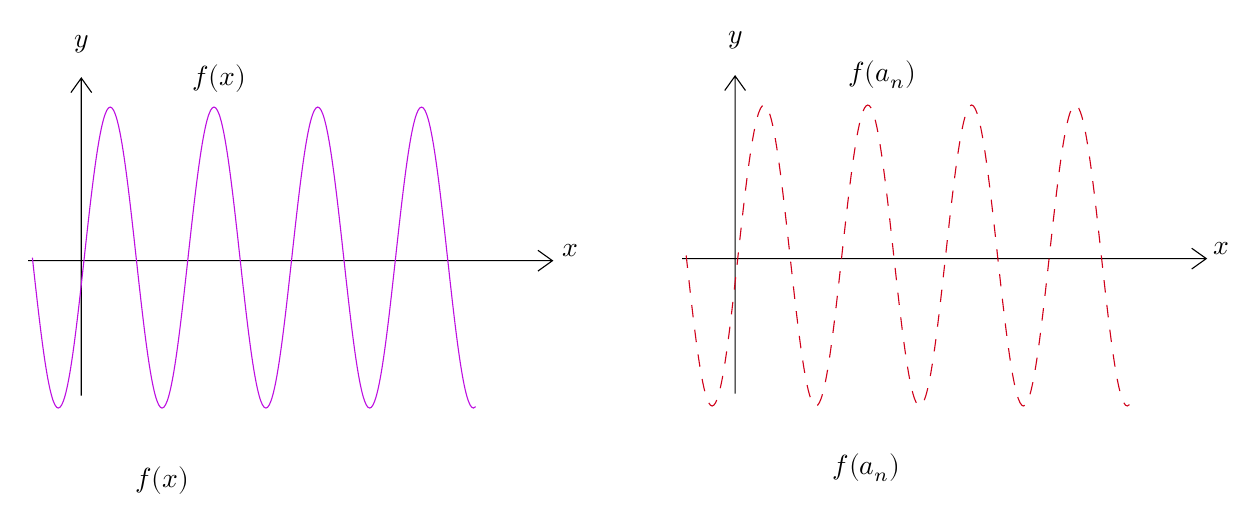
\begin{tikzpicture}[x=0.75pt,y=0.75pt,yscale=-1,xscale=1]
            \draw  (57,165) -- (309.57,165)(82.57,77) -- (82.57,230) (302.57,160) -- (309.57,165) -- (302.57,170) (77.57,84) -- (82.57,77) -- (87.57,84)  ;
            \draw  [color={rgb, 255:red, 189; green, 16; blue, 224 }  ,draw opacity=1 ] (59,163.5) .. controls (63.08,200.64) and (66.98,236) .. (71.5,236) .. controls (76.02,236) and (79.92,200.64) .. (84,163.5) .. controls (88.08,126.36) and (91.98,91) .. (96.5,91) .. controls (101.02,91) and (104.92,126.36) .. (109,163.5) .. controls (113.08,200.64) and (116.98,236) .. (121.5,236) .. controls (126.02,236) and (129.92,200.64) .. (134,163.5) .. controls (138.08,126.36) and (141.98,91) .. (146.5,91) .. controls (151.02,91) and (154.92,126.36) .. (159,163.5) .. controls (163.08,200.64) and (166.98,236) .. (171.5,236) .. controls (176.02,236) and (179.92,200.64) .. (184,163.5) .. controls (188.08,126.36) and (191.98,91) .. (196.5,91) .. controls (201.02,91) and (204.92,126.36) .. (209,163.5) .. controls (213.08,200.64) and (216.98,236) .. (221.5,236) .. controls (226.02,236) and (229.92,200.64) .. (234,163.5) .. controls (238.08,126.36) and (241.98,91) .. (246.5,91) .. controls (251.02,91) and (254.92,126.36) .. (259,163.5) .. controls (263.08,200.64) and (266.98,236) .. (271.5,236) .. controls (271.86,236) and (272.22,235.77) .. (272.57,235.34) ;
            \draw  (372,164) -- (624.57,164)(397.57,76) -- (397.57,229) (617.57,159) -- (624.57,164) -- (617.57,169) (392.57,83) -- (397.57,76) -- (402.57,83)  ;
            \draw  [color={rgb, 255:red, 208; green, 2; blue, 27 }  ,draw opacity=1 ][dash pattern={on 4.5pt off 4.5pt}] (374,162.5) .. controls (378.08,199.64) and (381.98,235) .. (386.5,235) .. controls (391.02,235) and (394.92,199.64) .. (399,162.5) .. controls (403.08,125.36) and (406.98,90) .. (411.5,90) .. controls (416.02,90) and (419.92,125.36) .. (424,162.5) .. controls (428.08,199.64) and (431.98,235) .. (436.5,235) .. controls (441.02,235) and (444.92,199.64) .. (449,162.5) .. controls (453.08,125.36) and (456.98,90) .. (461.5,90) .. controls (466.02,90) and (469.92,125.36) .. (474,162.5) .. controls (478.08,199.64) and (481.98,235) .. (486.5,235) .. controls (491.02,235) and (494.92,199.64) .. (499,162.5) .. controls (503.08,125.36) and (506.98,90) .. (511.5,90) .. controls (516.02,90) and (519.92,125.36) .. (524,162.5) .. controls (528.08,199.64) and (531.98,235) .. (536.5,235) .. controls (541.02,235) and (544.92,199.64) .. (549,162.5) .. controls (553.08,125.36) and (556.98,90) .. (561.5,90) .. controls (566.02,90) and (569.92,125.36) .. (574,162.5) .. controls (578.08,199.64) and (581.98,235) .. (586.5,235) .. controls (586.86,235) and (587.22,234.77) .. (587.57,234.34) ;
            \draw (78,55) node [anchor=north west][inner sep=0.75pt]   [align=left] {$\displaystyle y$};
            \draw (393,53) node [anchor=north west][inner sep=0.75pt]   [align=left] {$\displaystyle y$};
            \draw (313,156) node [anchor=north west][inner sep=0.75pt]   [align=left] {$\displaystyle x$};
            \draw (627,155) node [anchor=north west][inner sep=0.75pt]   [align=left] {$\displaystyle x$};
            \draw (100,263) node [anchor=north west][inner sep=0.75pt]   [align=left] {函数$\displaystyle f( x) 图像$};
            \draw (135,69.4) node [anchor=north west][inner sep=0.75pt]    {$f( x)$};
            \draw (451,67.4) node [anchor=north west][inner sep=0.75pt]    {$f( a_{n})$};
            \draw (436,257) node [anchor=north west][inner sep=0.75pt]   [align=left] {函数$\displaystyle f( a_{n}) 图像$};
        \end{tikzpicture}
    \end{center}
    \textcolor{red}{如上图所示$f(a_n)$其实是$f(x)$的抽样}
    \begin{center}
        \tikzset{every picture/.style={line width=0.75pt}} %set default line width to 0.75pt       
        \begin{tikzpicture}[x=0.75pt,y=0.75pt,yscale=-1,xscale=1]
        \draw  [color={rgb, 255:red, 189; green, 16; blue, 224 }  ,draw opacity=1 ] (59,163.5) .. controls (63.08,200.64) and (66.98,236) .. (71.5,236) .. controls (76.02,236) and (79.92,200.64) .. (84,163.5) .. controls (88.08,126.36) and (91.98,91) .. (96.5,91) .. controls (101.02,91) and (104.92,126.36) .. (109,163.5) .. controls (113.08,200.64) and (116.98,236) .. (121.5,236) .. controls (126.02,236) and (129.92,200.64) .. (134,163.5) .. controls (138.08,126.36) and (141.98,91) .. (146.5,91) .. controls (151.02,91) and (154.92,126.36) .. (159,163.5) .. controls (163.08,200.64) and (166.98,236) .. (171.5,236) .. controls (176.02,236) and (179.92,200.64) .. (184,163.5) .. controls (188.08,126.36) and (191.98,91) .. (196.5,91) .. controls (201.02,91) and (204.92,126.36) .. (209,163.5) .. controls (213.08,200.64) and (216.98,236) .. (221.5,236) .. controls (226.02,236) and (229.92,200.64) .. (234,163.5) .. controls (238.08,126.36) and (241.98,91) .. (246.5,91) .. controls (251.02,91) and (254.92,126.36) .. (259,163.5) .. controls (263.08,200.64) and (266.98,236) .. (271.5,236) .. controls (271.86,236) and (272.22,235.77) .. (272.57,235.34) ;
        \draw  [color={rgb, 255:red, 208; green, 2; blue, 27 }  ,draw opacity=1 ][dash pattern={on 4.5pt off 4.5pt}] (374,162.5) .. controls (378.08,199.64) and (381.98,235) .. (386.5,235) .. controls (391.02,235) and (394.92,199.64) .. (399,162.5) .. controls (403.08,125.36) and (406.98,90) .. (411.5,90) .. controls (416.02,90) and (419.92,125.36) .. (424,162.5) .. controls (428.08,199.64) and (431.98,235) .. (436.5,235) .. controls (441.02,235) and (444.92,199.64) .. (449,162.5) .. controls (453.08,125.36) and (456.98,90) .. (461.5,90) .. controls (466.02,90) and (469.92,125.36) .. (474,162.5) .. controls (478.08,199.64) and (481.98,235) .. (486.5,235) .. controls (491.02,235) and (494.92,199.64) .. (499,162.5) .. controls (503.08,125.36) and (506.98,90) .. (511.5,90) .. controls (516.02,90) and (519.92,125.36) .. (524,162.5) .. controls (528.08,199.64) and (531.98,235) .. (536.5,235) .. controls (541.02,235) and (544.92,199.64) .. (549,162.5) .. controls (553.08,125.36) and (556.98,90) .. (561.5,90) .. controls (566.02,90) and (569.92,125.36) .. (574,162.5) .. controls (578.08,199.64) and (581.98,235) .. (586.5,235) .. controls (586.86,235) and (587.22,234.77) .. (587.57,234.34) ;
        \draw (135,69.4) node [anchor=north west][inner sep=0.75pt]    {$f( x)$};
        \draw (451,67.4) node [anchor=north west][inner sep=0.75pt]    {$f( a_{n})$};
        \draw (88,247) node [anchor=north west][inner sep=0.75pt]   [align=left] {用$\displaystyle \upvarepsilon -\delta $求它的极限};
        \draw (396,252) node [anchor=north west][inner sep=0.75pt]   [align=left] {用海涅定理求它的极限};
        \end{tikzpicture}        
    \end{center}
    需要注意的是,是所有的数列(抽样)才能完全代表整体.不能说我选了某个数列有极限就代表函数有极限.
    总结:\textcolor{red}{海涅定理表述了离散与连续、数列极限与函数极限的关系.}
    \begin{problem}
        求$\lim_{n\to\infty}\sqrt[n]{\left(\cos\dfrac1{\sqrt{n}}\right)^{n^2}}.$
    \end{problem}
    \begin{solution}
        \begin{align*}
          \text{原式} & = \lim_{n\to \infty} \left( \cos\dfrac{1}{\sqrt{n}} \right)^n\\ 
          & = \lim_{n\to \infty} e^{n \ln \cos \dfrac{1}{\sqrt{n}}}\\
          & = \lim_{n\to \infty} e^{n \cos \left(\dfrac{1}{\sqrt{n}} - 1 \right)}\\
          & = \lim_{x\to+\infty}e^{x \left(\cos\dfrac{1}{\sqrt{x}}-1\right)} \\ 
          & = \lim_{x\to+\infty}e^{x \times \left[-\dfrac12{\left(\dfrac1{\sqrt{x}}\right)}^2\right]}=e^{-\dfrac12}
        \end{align*}
    \end{solution}
    \begin{note}
        本题有一个易错点在于$x\Bigg(\cos\dfrac{1}{\sqrt{x}}-1\Bigg)$的极限求解时,会认为括号内的极限为0,计算后的极限为0,导致错误
    \end{note}
    \begin{problem}
        求极限$\lim_{n \to \infty}n(\arctan n -\dfrac{\pi}{2})$
    \end{problem}
    \begin{solution}
          \begin{align*}
            \text{原式} & = \lim_{n \to \infty}\dfrac{\arctan n-\frac{\pi}{2}}{\frac{1}{n}} \\     
            & =  \lim_{x \to +\infty}\dfrac{\arctan x -\frac{\pi}{2}}{\frac{1}{x}}\\
            & = \lim_{x\to+\infty}\dfrac{\frac1{1+x^2}}{-\frac1{x^2}}\\
            & = -1
          \end{align*}  
    \end{solution}
    \begin{note}
        数列极限不可以直接使用洛必达法则,若要使用洛必达法则,则需要使用海涅定理进行替换.
    \end{note}
    \begin{problem}
        求极限$\lim_{n\to\infty}\left[\dfrac{\left(1+\frac1n\right)^n}{\mathrm{e}}\right]^n$   
    \end{problem}
    \begin{solution}
        \begin{align*}
          \text{原式} & = \lim_{n\to\infty}\left[\dfrac{\mathrm{e}^{n\ln\left(1+\frac1n\right)}}{\mathrm{e}}\right]^n    \\
          & = \lim_{n\to\infty}\dfrac{\mathrm{e}^{n^2\ln\left(1+\frac1n\right)}}{\mathrm{e^n}}\\
          & =\lim_{n \to \infty} e^{n^2\ln(1+\frac{1}{n})-n}
        \end{align*}
        对$\lim_{n \to \infty} n^2\ln(1+\dfrac{1}{n})-n$求极限得:
        \begin{align*}
          \text{原式} & = \lim_{n\to\infty}\biggl[n-n^2\ln\biggl(1+\frac{1}{n}\biggr)\biggr] \\
          & =  \lim_{n\to\infty}n^2\biggl[\frac{1}{n}-\ln\biggl(1+\frac{1}{n}\biggr)\biggr] \\
          & = \lim_{n\to\infty}n^2\cdot\frac12\left(\frac1n\right)^2 \\
          &= \dfrac{1}{2}
        \end{align*}
        综上函数极限为$e^{-\frac{1}{2}}$
    \end{solution}
    \begin{note}
        数列极限可以直接使用等价无穷小和泰勒公式
    \end{note}
    \begin{problem}
        \uline{求极限}$\lim_{n\to\infty}\tan^n\left(\dfrac\pi4+\dfrac2n\right)$
    \end{problem}
    \begin{solution}
        \begin{align*}
            \text{原式} & = \lim_{n\to\infty} e^{n \ln(\tan(\frac{\pi}{4}+\frac{2}{n}))}\\
            & =  \lim_{n\to\infty}e^{n\cdot (\tan(\frac{\pi}{4}+\frac{2}{n}) -1)}\\
            & = \lim_{n\to\infty}e^{n\cdot (\tan(\frac{\pi}{4}+\frac{2}{n}) -\tan \frac{\pi}{4})} \\
            & = \lim_{n\to\infty}e^{n \cdot \sec^2 \varepsilon \cdot \frac{2}{n}} \quad \varepsilon \in(\frac{\pi}{4},\frac{\pi}{4}+\frac{2}{n})\\
            &=e^4
        \end{align*}
    \end{solution}
    \begin{note}
        数列极限可以使用拉格朗日中值定理
    \end{note}
    \section{无穷小与无穷大}
    \subsection{无穷小}
    \begin{defn}{无穷小的定义}{}
        如果函数$f(x)$当$x\to x_0$(或 $x\to\infty$)时的极限为零,那么称函数$f(x)$为当$x\to x_0$(或$x\to\infty$)时的无穷小.
    \end{defn}
    \textcolor{red}{$f(x)$是可以本身为$0$或者无限趋近于零,其中$0$可以作为无穷小唯一常数}.
    \begin{criterion}{无穷小与函数极限的关系(脱帽法)}{}
        $\lim_{x\to\cdot}f(x)=A\Leftrightarrow f(x)=A+\alpha$,其中$\lim_{x\to\cdot}f(x)$为超实数值,其实数部分为$A$,函数$f(x)$的函数值为$A+\alpha$\label{wqx1}
    \end{criterion}
    \subsubsection{\textcolor{red}{无穷小的性质}}
    \begin{itemize}
        \item[1] 有限个无穷小的和是无穷小\footnote{无穷个无穷小的和不一定是无穷小,如$\lim_{n \to \infty}=(\dfrac{1}{n+1}+\dfrac{1}{n+2}+\dfrac{1}{n+3}\dots +\dfrac{1}{n+n})=\ln 2$}
            \begin{proof}
                设$\alpha_1$和$\alpha_2$为无穷小量.则$0 \leqslant |\alpha_1+\alpha_2|\leqslant |\alpha_1|+|\alpha_2|$,$|\alpha_1|+|\alpha_2|$的极限为0.证明完毕.
            \end{proof}
        \item[2] 有界函数与无穷小的乘积是无穷小\footnote{无界函数$\times$无穷小量不一定是无穷小,如$\lim_{x \to \infty}x \times \dfrac{1}{x}=1$}
            \begin{proof}
                $|\alpha _1|\leqslant M$,$\alpha_2$是无穷小量.那么$0\leqslant|\alpha_1 \times \alpha_2|=|\alpha_1|\times |\alpha_2|\leqslant M \times |\alpha_2|$证明完毕.
            \end{proof}
        \item[3] 有限个无穷小的乘积是无穷小\footnote{这个地方虽然张宇老师给出了证明,但是好像存在一定的争议性}
    \end{itemize}
    \subsubsection{\textcolor{red}{无穷小的比阶}}
    \begin{defn}{不同无穷小的比阶}{}
        \begin{itemize}
            \item 如果 $\lim \dfrac{\beta}{\alpha} =0$,那么就说 $\beta$是比$\alpha$高阶的无穷小,记作 $\beta=o(\alpha);$
            \item  如果 $\lim \dfrac\beta\alpha  =\infty$,那么就说 $\beta$是比 $\alpha$低阶的无穷小;
            \item 如果$\lim\dfrac{\beta}{\alpha} =c\neq 0$,那么就说 $\beta$ 与 $\alpha$ 是同阶无穷小 ;
            \item 如果$\lim\dfrac{\beta}{\alpha^{^k}} =c \neq 0$,$k > 0$,那么就说 $\beta$是关于 $\alpha$的$k$阶无穷小\footnote{不是相等,超实数系下没有加减运算,只可以进行替换运算};
            \item 如果 $\lim \dfrac\beta\alpha = 1$,那么就说 $\beta$ 与 $\alpha$ 是等价无穷小,记作 $\alpha\sim\beta$
        \end{itemize}
    \end{defn}
    前三个定义解释:$\lim \dfrac{\beta}{\alpha} =0$是指分子趋于$0$的速度比分母快,$\lim \dfrac\beta\alpha =\infty$是指分子趋于$0$的速度比分母慢,$\lim\dfrac{\beta}{\alpha} =c\neq 0$是指趋于$0$的速度一样.同时需要注意的是,\textcolor{red}{并不是任意两个无穷小都可进行比阶的}\footnote{例如,当 $x\to 0$ 时,$x\sin\dfrac1x$与$x^2$虽然都是无穷小,但是却不可以比阶,也就是说既无高低阶之分,也无同阶可言,因为$\lim_{x \to 0}\dfrac{x \sin \dfrac{1}{x}}{x^2}=\lim_{x\to0}\dfrac1x\sin\dfrac1x$不存在,其值为$\infty$和$0$}.
    \newline
    \textbf{对$o(x)$的理解}:它是一个无穷小,但是它趋向于0的速度比 $x$ 要快,也就是$\lim_{x\to0}\dfrac{o(x)}{x}=0$ ,也就是精度更高.举一个实际的例子:$\tan x=x+\dfrac13x^3+\dfrac2{15}x^5+o\left(x^5\right)$, 那么就应该知道$\tan x-x-\dfrac{1}{3}x^{3}-\dfrac{2}{15}x^{5}=o\left(x^{5}\right)$,也就是这玩意趋于0 的速度非常之快!速度相当于 $x^5$ ,这给我们的精度分析提供了一些帮助. 由此可以解释加减法不推荐用等价无穷小,例如$\lim_{x\to0}\dfrac{\tan x-x}{x^3}\neq\lim_{x\to0}\dfrac{x-x}{x^3}$等价无穷小本身就是一种近似替换,直接把 $\tan x$ 近似成 $x$ 显然精度太低 (毕竟分母可是以 $x^3$ 的速度趋于0), 那么我们就需要更高精度的近似了,也就是 $\lim_{x\to0}\dfrac{\tan x-x}{x^3}=\lim_{x\to0}\dfrac{x+\frac13x^3+o\left(x^3\right)-x}{x^3}$, 这样我们就得到 $\lim_{x\to0}\dfrac{\tan x-x}{x^3}=\dfrac13+\lim_{x\to0}\dfrac{o(x^5)}{x^3}$, 显然,后者分子趋于0的速度大概是 $x^5$ 级别比分母更快所以忽略不计.
    \begin{conclusion}{无穷小比阶的结论}{}
        若 $f(x)$ 在 $x=0$ 的某邻域内连续,且当$x\to0$ 时 $f(x)$ 是$x$的$m$ 阶无穷小,$\varphi(x)$ 是$x$ 的$n$阶无穷小,则当$x\to0$ 时$F( x) = \int _0^{\varphi(x)}f(t)$d$t$ 是$x$ 的$n(m+1)$阶无穷小
    \end{conclusion}
    \begin{problem}
        把$x\to 0^+$时的无穷小$a= \int _0^x \cos t^2dt$, $\beta= \int _0^{x^2} \tan\sqrt{t} dt$, $\gamma= \int _0^{\sqrt{x}} \sin t^3 dt$进行排序,使排在后面的是前一个的高阶无穷小,则正确的排列顺序是
    \end{problem}
    \begin{solution}
        $\alpha$:$n=1,\lim_{x\to 0} \cos x^2=1$,因此$m=0$,那么$n(m+1)=1$;$\beta$:$n=2,m=\dfrac{1}{2}$,那么$n(m+1)=3$.$\gamma$:$m=\dfrac{1}{2}x,n=2$,那么$n(m+1)=2$.因此顺序为$\alpha \gamma \beta$
    \end{solution}
    \begin{problem}
        当 $x\to0$ 时,下列无穷小中最高阶的是:\\
        $\left(A\right)\left(2+\tan x\right)^{x}-2^{x}$ \qquad $\left(B\right)\left(\cos x^{2}\right)^{\frac{1}{x}}-1$ \qquad $( C) \int _0^{1- \cos x}e^{x}\sin t^2$d$t$ \qquad$\left(D\right)\int_{\sin x}^{1-\sqrt{\cos x}}\ln(1+t^{3})dt$
    \end{problem}
    \begin{solution}
        A选项:$2^x[(1+\dfrac{\tan x}{2})^x-1]=\dfrac{\tan x}{2}\times x=\dfrac{1}{2}x^2$.\\
        B选项:$-\dfrac{x^4}{2x}=-\dfrac{x^3}{2}$.\\
        C选项:$n=\dfrac{1}{2}x^2,m=x^2$那么$n(m+1)=6$.\\
        D选项:\begin{align*}
          \text{原式} & = \int_{\sin x}^{1-\sqrt{\cos x}}\ln(1+t^3) \mathrm{d}t \\
          & = \int_{\sin x}^0\ln(1+t^3) \mathrm{d}t+\int_0^{1-\sqrt{\cos x}}\ln(1+t^3) \mathrm{d}t \\
          & = \int_{0}^{1-\sqrt{\cos x}}\ln(1+t^{3})\mathrm{d}t-\int_{0}^{\sin x}\ln(1+t^{3})dt
        \end{align*}
        其中$1-\sqrt{\cos x}\sim\dfrac{\frac12x^2}2$,那么$\int_0^{1-\sqrt{\cos x}}\ln(1+t^3) \mathrm{d}t$
        那么$n(m+1)=8$,$\int_0^{\sin x}\ln\left(1+t^3\right)\mathrm{d}t$那么$n(m+1)=8$,$\int_{\sin x}^{1-\sqrt{\cos x}}\ln(1+t^3) \mathrm{d}t.$的阶数为4.综上C选项的阶数最高.
    \end{solution}
    \begin{note}
        D选项:如果为变上下限的形式,则转化为变上限的形式,然后使用结论进行计算,之后按照无穷小的运算法则计算即可.
    \end{note}
    \begin{problem}
        设 $p(x)=a+bx+cx^2+dx^3$.当$x\to0$ 时,若 $p(x)-\tan x$ 是比$x^{3}$ 高阶的无穷小,则下列结论中错误的是:\\
        $(A)a=0 \qquad (B)b=1 \qquad (C)c=0 \qquad (D)d=\dfrac{1}{6}$
    \end{problem}
    \begin{solution}
        对$\dfrac{p(x)-\tan x}{x^3}$泰勒展开可得:$\dfrac{p(x)-(x+\frac13x^3+\frac2{15}x^5)}{x^3}=\dfrac{a+bx+cx^2+dx^3-x-\frac{1}{3}x^3-\frac{2}{15}x^5}{x^3}$\\
        综上易知:$a=0,b=1,c=0,d=\dfrac{1}{3}$.因此,D选项是错误的.
    \end{solution}
    \begin{problem}
        \uline{当$x\to0^+$时,下列无穷小量中最高阶的是} \\
        $(A)\int _0^{x^2}\ln ( 1+ {\sqrt {t}}) $d$t \qquad (B) \int_{x^{3}}^{x^{2}}\sqrt{1-\sqrt{\cos t}}\:\mathrm{d}t \qquad (C)\int _x^{2\sin x}\sin t^2$d$t \qquad (D) \int _x^{\sin x}( \mathrm{e} ^{t^2}- 1) $d$t$  
    \end{problem}
    \begin{solution}
        A:$\ln(1+\sqrt{x}) \sim \sqrt{x}$,其$n(m+1)=3$.\\B:$\sqrt{1-\sqrt{\cos t}}=\dfrac{1}{2}x,$其$n(m+1)$的最小值为4.\\C:使用积分中值定理可得:$\sin^2 \varepsilon \times (2\sin x- x),\varepsilon \in (2\sin x,x)$,使用等价无穷小可得:$2\sin x-x \sim x,\sin^2 \varepsilon \sim \varepsilon ^2 \sim x^2$,那么其最终化为$x^3$.\\D选项:$(\sin x - x)(e^{\varepsilon ^2}-1),\varepsilon \in (\sin x,x)$.使用等价无穷小可得:$(-\dfrac{1}{6}x^5 \times \varepsilon)\sim x^6$. 最终选择D选项.
    \end{solution}
    \begin{note}
        如果上下限同阶的情况,如本题的C,D选项,则不可进行拆分,需要使用积分中值定理\ref{jfzz1}进行计算.
    \end{note}
    \subsubsection{无穷小的运算}\footnote{此处多用于泰勒公式的应用中,会对上述高阶无穷小的运算提出要求}
    设$m,n$为无穷小,则
    \begin{itemize}
        \item[1.] $o(x^{m})\pm o(x^{n})=o(x^{l}),l=\min\{m,n\}$
        \item[2.] $o(x^{m})\cdot o(x^{n})=o(x^{m+n}),x^{m}\cdot o(x^{n})=o(x^{m+n})$
        \item[3.] $o(x^{m})=o(kx^{m})=k\cdot o(x^{m}),k \neq 0$
    \end{itemize}
    \begin{problem}
        若当$x\to0$时,$\alpha(x),\beta(x)$是非零无穷小量,则以下的命题中正确的是:\\
        A.若$\alpha(x)\sim\beta(x)$,则$\alpha^2(x)-\beta^2(x);$\quad B.若$\alpha^2(x)\sim\beta^2(x)$,则$\alpha(x)\sim\beta(x);$ \\ C.若$\alpha(x)\sim\beta(x)$,则$\alpha(x)-\beta(x)=o(\alpha(x));$ \quad D.若$\alpha(x) \sim \beta(x)=o(\alpha(x))$,则$\alpha(x)~-\beta(x)$
    \end{problem}
    \begin{solution}
        \begin{enumerate}
            \item $\lim_{x \to 0}\dfrac{\alpha(x)}{\beta(x)}=1$,那么$\lim_{x \to 0}[\dfrac{\alpha(x)}{\beta(x)}]^2=1$
            \item $\lim_{x\to 0}\dfrac{\alpha(x)^2}{\beta(x)^2}=1 \Rightarrow \lim_{x \to 0}\dfrac{\alpha(x)}{\beta(x)} = \pm 1$
            \item $\lim_{x \to 0}\dfrac{\alpha(x)-\beta(x)}{\beta(x)}=0$
            \item $\lim_{x\to 0}\dfrac{\alpha(x)-\beta(x)}{\beta(x)}=1$
        \end{enumerate}
    \end{solution}
    \begin{note}
        \textcolor{red}{若$\alpha(x) \sim \beta (x)$,那么$\lim_{x \to 0}\dfrac{\alpha(x)}{\beta(x)}=1 \Leftrightarrow \lim_{x\to 0}\dfrac{\beta(x)}{\alpha(x)}$}
    \end{note}
    \begin{problem}
        设对任意的$x$总有$\varphi(x)\leqslant f(x)\leqslant g(x)$,且$\lim_{x\to \infty}[g(x)-\varphi(x)]=0$,则$\lim_{x\to \infty}f(x)$\\
        (A)存在且等于零.\quad (B) 存在但不一定为零.\quad(C)一定不存在.\quad(D)不一定存在
    \end{problem}
    \begin{solution}
        令$\varphi(x)=f(x)=g(x)=\begin{cases} x\\1\\0 \end{cases}$,易知D选项正确
    \end{solution}
    \begin{note}
        \textcolor{red}{遇见$\leq$,$\geq$的形式,可以一律取$=$}
    \end{note}
    \subsection{无穷大}
    \begin{defn}{无穷大的定义}{}
        设函数$f(x)$在$x_0$的某一去心邻域内有定义(或$|x|$大于来一正数时有定义).如果对于任意给定的正数$M$(不论它多么大),总存在正数$\delta$(或数$X$),只要$x$适合不等式$0<|x-x_0|<\delta$(或$|x|>X$),对应的函数值$f(x)$总满足不等式
        $$
            |f(x)|>M
        $$
        那么称函数$f(x)$是当$x\to x_0$(或$x\to\infty$\footnote{等价于$x \to -\infty$同时$x \to +\infty$})时的无穷大.\footnote{\textcolor{red}{无穷大一定无界,但无界不一定是无穷大量.}与无穷小相同,都是一个极限过程,因此无穷大也是一个极限,所以无界不一定是无穷大量}
        其$\varepsilon-N$语言为
        $$
            \lim\limits_{x\to x_0}f(x)= \infty \Leftrightarrow\forall M >0,\exists\delta>0,\text{当}0<|x-x_0|<\delta\text{时},\text{有}|f(x)|>M.
        $$
    \end{defn}
    \subsubsection{\textcolor{red}{无穷大的比阶}}
    \begin{itemize}
        \item 当$x \to +\infty$时,$\mathrm{ln}^ax\ll x^\beta\ll a^x,\text{其中}\alpha>0,\beta>0,a>1.$\footnote{由洛必达公式证明}
        \item 当$n \to \infty$时,$\ln^an\ll n^\beta\ll a^n\ll n!\ll n^n,\text{其中 }\alpha>0,\beta>0,a>1.$
    \end{itemize}
    \subsubsection{\textcolor{red}{无穷大的性质}}
    \begin{itemize}
        \item 两个无穷大量的积仍未无穷大量
        \item 无穷大量与有界变量的和仍是无穷大量
    \end{itemize}
    \subsubsection{无穷大与无界变量的关系}
    无穷大量一定是无界变量,但无界变量不一定是无穷大量.\footnote{如数列$x_n=\begin{cases}n,n\text{ 为奇数}\\0,n\text{ 为偶数}&\end{cases}$,是无界变量,但不是无穷大.无穷大是一个极限}
    \subsection{无穷大与无穷小的关系}
    在自变量的同一变化过程中,若$f(x)$是无穷大,则$\dfrac{1}{f(x)}$是无穷小;若$f(x)$是无穷小,且$f(x)\neq 0$,则$\dfrac{1}{f(x)}$是无穷大.
    \subsubsection{无穷小$\times \infty$的值}
    \textbf{无穷小$\times \infty$的值是一个为定式}.因为低阶无穷小乘以高阶无穷大等于无穷大,高阶无穷小乘以低阶无穷大等于 0,同阶无穷小和无穷大相乘等于 1.比如:
    $$
        \lim_{x\to0}x\cdot \ln x=0 
    $$
    $$
        \lim_{x\to0}x\cdot\dfrac1{\sin x}=1 
    $$
    $$
        \lim_{x\to0}x\cdot\dfrac1{x^2}=\infty 
    $$
    \section{函数极限的运算}
    \subsection{极限的四则运算法则}\label{jxdsz1}
    \subsubsection{\textcolor{red}{利用极限的四则运算法则求极限}}\footnote{易错,在计算中往往容易忽视极限不存在的情况}
    如果极限不存在,那么极限属于超实数系的范畴,在超实数系下不可以进行代数运算,只可以进行替换运算.\textcolor{red}{但是如果极限均存在,那么可以进行代数计算}.那么就可以使用下面的运算法则:\\
    若$\lim f(x)=A$,$\lim g(x)=B$,那么
    \begin{itemize}
        \item $\operatorname*{lim}[kf(x)\pm lg(x)]=k\operatorname*{lim}f(x)\pm l\operatorname*{lim}g(x)=kA\pm lB$,其中$k,l$为常数
        \item $\operatorname*{lim}[f(x)\cdot g(x)]=\operatorname*{lim}f(x)\cdot\operatorname*{lim}g(x)\equiv A\cdot B$,特别的,若$\lim f(x)$存在,$n$为正整数,则$\operatorname{lim}[f(x)]^n=\begin{bmatrix}\operatorname{lim}f(x)\end{bmatrix}^n$
        \item $\operatorname*{lim}\dfrac{f(x)}{g(x)}=\dfrac{\operatorname*{lim}f(x)}{\operatorname*{lim}g(x)}=\dfrac{A}{B}(B\neq0)$
    \end{itemize}
    \begin{criterion}{常用结论}{}
        \begin{table}[H]
            \begin{center}
                \begin{tabular}{l|l}
                    \text{存在} \pm \text{不存在} = \text{不存在}\footnote{只有这一个是\text{不存在},其余都是不一定或者存在} & \text{不存在} \pm \text{不存在} =\text{不一定}\footnote{反例:$\lim _{x \to 0}(\sin \dfrac{1}{x}-\sin \dfrac{1}{x})=0$} \\ \hline
                    \text{存在} \times (\div) \text{不存在} = \text{不一定} & \text{不存在} \times(\div) \text{不存在} = \text{不一定}
                \end{tabular}
            \end{center}
        \end{table}
    \end{criterion}
    \begin{problem}
        \begin{enumerate}
            \item 证明:$\lim f(x)=A \neq 0 \Rightarrow \lim f(x)g(x)=A \lim g(x)$
            \item 证明:$\lim \dfrac{f(x)}{g(x)}$存在,$\lim g(x)=0 \Rightarrow \lim f(x)=0$
            \item 证明:若$\lim_{x \to x_0}g(x)=A,\lim_{x \to A}f(x)=B$,能否推出$\lim_{x\to x_0}f(g(x))=B$,若不能,则满足什么条件可以推出该结论?
        \end{enumerate}
    \end{problem}
    \begin{proof}
        \begin{enumerate}
            \item $\lim f(x)=\lim\dfrac{f(x)}{g(x)}\cdot g(x)=\lim\dfrac{f(x)}{g(x)}\cdot\lim g(x)=A\cdot0=0.$
            \item \textbf{由于$g(x)=\dfrac{f(x)}{\frac{f(x)}{g(x)}}$,则$\lim g(x)=\lim\dfrac{f(x)}{\frac{f(x)}{g(x)}}=\dfrac{\lim f(x)}{\lim\frac{f(x)}{g(x)}}=\dfrac{0}{A}=0$}
            \item 无法推出,有如下反例
            \begin{itemize}
                \item $g(x)=x \sin \dfrac{1}{x},f(x)=\begin{cases} x,x \neq 0\\1,x=0 \end{cases}$,$\lim_{x \to 0}g(x)=0,\lim_{x\to0}f(x)=0$,但是当$x \to 0$时,$g(x)=x\sin \frac{1}{x}$不仅趋于0,同时还能在$\dfrac{1}{n \pi}$这样的点处严格等于0.此时$\lim_{x \to 0}f(g(x))=1$,所以$\lim_{x\to 0}f(g(x))$不存在,其极限值在$(0,1)$之间反复横跳.
                \item $g(x) \equiv 0$,$f(x)=\begin{cases} x,x \neq 0\\ 1,x=0 \end{cases}$,$\lim_{x\to 0}g(x)=0,\lim_{x\to 0}f(x)=0.$但$\lim_{x\to 0}f(g(x))=1$
            \end{itemize}
            因此结论不成立.若要成立,则应改为:
            \begin{itemize}
                \item 若$\lim_{x \to x_0}g(x)=A,\lim_{x\to A}f(x)=B$,且$g(x)\neq A$,则$\lim_{x\to x_0}f(g(x))=B$
                \item 若$\lim_{x \to x_0}g(x)=A,\lim_{x\to A}f(x)=B$,即$f(x)$在$x=A$处连续,则$\lim_{x\to x_0}f(g(x))=B$
            \end{itemize}
        \end{enumerate}
    \end{proof}
    \begin{conclusion}{上题的三个结论}{}
        \begin{itemize}
            \item $\lim f(x)=\lim\dfrac{f(x)}{g(x)}\cdot g(x)=\lim\dfrac{f(x)}{g(x)}\cdot\lim g(x)=A\cdot0=0.$
            \item \textcolor{red}{若$\lim_{x \to x_0}g(x)=A,\lim_{x\to A}f(x)=B$,且$g(x)\neq A$}\footnote{从根本上排除了常值函数和振荡间断点的反例},\textcolor{red}{则$\lim_{x\to x_0}f(g(x))=B$}
            \item \textcolor{red}{若$\lim_{x \to x_0}g(x)=A,\lim_{x\to A}f(x)=B$,即$f(x)$在$x=A$处连续}\footnote{\textcolor{red}{不管内函数能否取到极限值,只要外函数连续,复合之后极限一定存在}},\textcolor{red}{则$\lim_{x\to x_0}f(g(x))=B$}
        \end{itemize}
    \end{conclusion}
    \begin{problem}
        求$\lim_{x\to+\infty}\dfrac{e^x}{\left(1+\dfrac1x\right)^{x^2}}.$极限
    \end{problem}
    \begin{solution}
        由于该极限的分子$e^x$的极限为无穷大,无穷大属于极限中的不存在情况,因此不可以使用极限的四则运算法则\ref{jxdsz1},也不可以对分母使用两个重要无穷小进行化简.只能使用等价变换进行求解.即
        \begin{align*}
           \text{原式} & =\lim_{x\to +\infty}\dfrac{e^x}{e^{x^2 \ln (1+\frac{1}{x})}}\\
           & =\lim_{x\to +\infty} e^{x-x^2\ln(1+\frac{1}{x})}\\
           & \xlongequal{\text{泰勒展开}}\lim_{x\to +\infty} e^{x-x+\frac{1}{2}}\\
           & =e^{\frac{1}{2}}
        \end{align*}
    \end{solution}
    \begin{problem}
        \uline{已知$f(0)=f'(0)=0$,$f''(0)\neq0$,求}$\lim _{x \to 0}\dfrac{\frac{f(x)}{x}}{f'(x)}$
    \end{problem}
    \begin{solution}
        如果想把分子写$x \to 0$时的导数形式,然后进行计算,即$\lim_{x \to 0}\dfrac{\frac{f(x)-f(0)}{x-0}}{f'(0)}=\dfrac{f'(0)}{f'(0)}=1$进行运算,则不满足极限四则运算法则\ref{jxdsz1},因为其分母为0,违背了极限的四则运算法则,因此不可这样计算,需要对其进行恒等变形计算.即
        \begin{equation*}
            \begin{split}
                \text{原式} & =\lim_{x \to 0}\dfrac{\dfrac{f(x)}{x^2}}{\dfrac{f'(x)-f'(0)}{x}} \\
                & =\dfrac{1}{f''(0)}\lim_{x \to x_0}\dfrac{f(x)}{x^2} \\
                & \xlongequal {\text{洛必达法则}}\frac{1}{f''(0)}\lim_{x\to 0}\dfrac{1}{2}\dfrac{f'(x)-f'(0)}{x}\quad (\text{易错:此处的处理不可再次使用洛必达,因为二阶导在此不连续})  \\
                & =\frac{1}{f''(0)}\dfrac{1}{2}f''(0) \\
                & =\dfrac{1}{2} \\
            \end{split}
        \end{equation*} 
    \end{solution}
    \begin{note}
        \textcolor{red}{使用极限运算法则的注意事项}:在求分式这种形式的极限时,一定要注意分子的极限是不是无穷,如果极限为无穷则不可以使用极限运算法则对极限进行拆分计算,同时还要注意分母的极限是不是0,如果是0,则也不可以使用极限运算法则计算,只能进行等价替换进行运算.
    \end{note}
    \begin{problem}
        求$\lim_{x\to 0}(\dfrac{1}{x^2}-\cot^2 x)$    
    \end{problem}
    \begin{solution}
        \begin{equation*}
            \begin{split}    
                \text{原式} &= \lim_{x \to 0}(\dfrac{1}{x^2}-\dfrac{1}{\tan^x x}) \\
                & =\dfrac{(\tan x +x)(\tan x - x)}{x^2 \times \tan^2 x} \\
                & =\dfrac{2x \times \dfrac{1}{3}x^3}{x^4} \\
                & =\dfrac{2}{3} \\
            \end{split}
        \end{equation*} 
    \end{solution}
    \begin{note}
        本题的有另一个解法,但是相较上面的解法相比有些复杂,但是记录一个常见的错误,即什么时候可以用等价无穷小的问题,其写法为:
      \begin{align*}
         \text{原式} & = \lim_{x\to 0}(\dfrac{1}{x^2}-\cot ^2 x)=(\dfrac{1}{x^2}-\dfrac{\cos^2 x}{\sin^2 x})  & \\ 
        & =\lim_{x\to 0}\dfrac{\sin^2 x-x^2 \cos^2 x}{x^2 \sin^2 x} & \\
        & =\lim_{x\to 0}(\dfrac{\sin^2 x-x^2\cos^2x}{x^4})
    \end{align*}
    此处有一个常见的错误,就是能不能把 $\cos^2 x$代换为1,其实是不能的,即使最后答案正确,此时$x \to 0$时,分母也趋于0,如果进行替换,则违背了极限的运算法则,因此不能进行替换
        \begin{align*}
            \text{原式} & =  \lim_{x\to 0}\dfrac{(\sin x-x\cos x)(\sin x+x\cos x)}{x^4}\xlongequal {\text{泰勒公式}}\dfrac{2}{3} 
        \end{align*}
    \end{note}
    \subsection{泰勒公式}
    \textcolor{red}{泰勒公式的目的是提高精确度,用更高次的多项式来逼近函数}
    \subsubsection{带拉格朗日余项的$n$阶泰勒展开式}
    如果函数$f(x)$在\textbf{$x_0$的某个邻域$U(x_0)$内具有(n +1)阶导数},那么对任一$x\in U(x_0)$,有
    $$
    f(x)=f(x_{0})+f^{\prime}(x_{0})(x-x_{0})+\dfrac{f^{\prime\prime}(x_{0})}{2!}(x-x_{0})^{2}+\dfrac{f^{(n)}\left(x_{0}\right)}{n!}\left(x-x_{0}\right)^{n}+{\dfrac{f^{(n+1)}(\xi)}{(n+1)!}}(x-x_{0})^{n+1}
    $$
    \subsubsection{带佩亚诺余项的$n$阶泰勒展开式}
    如果函数$f(x)$在\textbf{$x_0$处具有$n$ 阶导数,那么存在$x_{0}$的一个邻域,对于该邻域内的任一 $x$},有
    $$
    f(x)=f(x_{0})+f'(x_{0})(x-x_{0})+\dfrac{f''(x_{0})}{2!}(x-x_{0})^{2}+\cdots+\dfrac{f^{(n)}(x_{0})}{n!}(x-x_{0})^{n}+o\left(\left(x-x_{0}\right)^{n}\right)
    $$
    \subsubsection{带有佩亚诺余项的麦克劳林公式}
    对带有佩亚诺余项的泰勒公式取$x_0=0$,则可以得到带有佩亚诺余项的麦克劳林公式\footnote{此处有一个易被忽略的地方,只有函数在$x_0$处,$n$阶导数存在,才可以展开到$n$阶}
    $$
    f(x)=f(0)+f'(0)x+\cdots+\dfrac{f^{(n)}(0)}{n!}x^{n}+o(x^{n})
    $$
    当$x\to 0$时,由带有佩亚诺余项的麦克劳林公式可得,有以下结论
    \begin{align*}
        \boxed{\begin{aligned}
                    & \sin x =x-\dfrac{x^3}{3!}+o(x^3)                                &  & \cos x =1-\dfrac{x^2}{2!}+\dfrac{x^4}{4!}+o(x^4)                  \\
                    & \arcsin x =x+\dfrac{x^3}{3!}+o(x^3)                             &  &                              \arccos x=\frac\pi2-\arcsin x=\frac\pi2-x-\frac1{3!}x^3+o(x^3)       \\
                    & \arctan x =x-\dfrac{x^{3}}{3}+o(x^{3})                          &  & \tan x =x+\dfrac{x^3}3+o(x^3)              \\
                    & \mathrm{e}^{x} =1+x+\dfrac{x^{2}}{2!}+\dfrac{x^{3}}{3!}+o(x^{3}) &  & (1+x)^{a} =1+\alpha x+\dfrac{\alpha(\alpha-1)}{2!}x^{2}+o(x^{2}) \\
                    & \dfrac{1}{1+x}=1-x+x^{2}-\cdots+(-1)^{n}x^{n}+o(x^{n})          &  &       \dfrac{1}{1-x}=1+x+x^{2}+\cdots+x^{n}+o(x^{n}) \\
                    & \ln (x+\sqrt{1+x^{2}})=x-\dfrac{1}{6}x^{3}+\dfrac{3}{40}x^{5}+\cdots \footnotemark[1]   & & \ln(1+x) =x-\dfrac{x^{2}}{2}+\dfrac{x^{3}}{3}+o(x^{3}) 
                \end{aligned}}
    \end{align*}
    \footnotetext[1]{该函数为反双曲正弦函数}
    \begin{criterion}{泰勒公式应用时的展开原则\label{tlgsyy}}{}
        \begin{itemize}
            \item $\dfrac{A}{B}$型,适用于"上下同阶"原则:具体来说,如果分母或者分子是$x$的$k$次幂,则应把分子或分母展开到$x$的$k$次幂.如:$\lim_{x\to0}\dfrac{x-\ln(1+x)}{x^{2}}$,此处$\ln(1+x)$应展开为$x-\dfrac{x^2}{2}+o(x^2)$
            \item $A-B$型,适用"幂次最低"原则:将$A,B$分别展开到他们系数不相等的$x$的最低次幂为止.如:已知当$x\to0$时,$\cos x-e^{\frac{x^2}2}$与$ax^b$为等价无穷小,求$a,b$.则应展开为$\cos x=1-\dfrac{x^2}{2!}+\dfrac{x^4}{4!}+o(x^4),\mathrm{e}^{-\frac{x^2}{2}}=1-\dfrac{x^2}{2}+\dfrac{1}{2!}\dfrac{x^4}{4}+o(x^4).$
        \end{itemize}
    \end{criterion}
    \begin{criterion}{泰勒公式的解题技巧}{}
        \begin{enumerate}
            \item \textcolor{red}{泰勒公式构建了函数与其高阶导之间的联系,因此看见高阶导数,要条件反射的想到泰勒公式}
            \item 奇函数的泰勒展式只有奇数次幂,偶函数的泰勒展式只有偶数次幂\footnote{如$\sin x$和$\cos x$}
            \item 极限当中,用佩亚诺余项$O$($x$的$n$次幂),证明题中,用拉格朗日余项,找提供信息最多的点作为展开点
            \item 等价无穷小的本质是泰勒的低精度形式,加减法不建议使用等价无穷小,建议直接泰勒
            \item 加项减项的本质也是泰勒\footnote{如$\ln(x)=\ln(1+x-1)\sim x-1$}
        \end{enumerate}
    \end{criterion}
    \begin{problem}
        $\lim_{x\to 0}\dfrac{e^x \sin x-x(1+x)}{x^2\sin x}$
    \end{problem}
    \begin{solution}
        \begin{align*}
          \text{原式} & = \lim_{x \to 0} \dfrac{\left[1+x+\frac12x^2+\frac16x^3+o(x^3)\right]\left[x-\frac16x^3+o(x^3)\right]-x(1+x)}{x^3} \\
          & = \lim_{x\to0}\dfrac{\left(-\frac{1}{6}+\frac{1}{2}\right)x^3+o\left(x^3\right)}{x^3}\\
          & = \dfrac13
        \end{align*}
    \end{solution}
    \begin{note}
        有的题可能泰勒公式之后多几个高阶的,但是还是应该遵循泰勒公式展开原则\ref{tlgsyy}
    \end{note}
    \begin{problem}
        $\lim_{x\to0}\dfrac{\ln\left(1+x+x^{2}\right)-x}{x^{2}}$
    \end{problem}
    \begin{solution}
        对等式进行泰勒展开即:$$\dfrac{\ln(1+x+x^2)-x}{x^2}=\dfrac{(x+x^2-\dfrac{1}{2}(x+x^2)^2-x)}{x^2}=\lim_{x \to 0}\dfrac{x^2-\dfrac{1}{2}x^2}{x^2}=\dfrac{1}{2}$$
    \end{solution}
    \begin{problem}
        $f(x)$在$x=0$处二阶可导且满足$\lim_{x\to 0}\dfrac{f(x)\sin x+\ln(1+x)}{x^3}=0$ ,求$f(0),f^{\prime}(0),f^{\prime\prime}(0)$
    \end{problem}
    \begin{solution}
        对原式中$f(x)$和$\sin x$和$\ln(1+x)$各项进行泰勒展开得:
    \begin{equation*}
        \begin{split}    
            & \lim_{x\to 0}\dfrac{f(x)\sin x+\ln(1+x)}{x^3}=0 \\
            & = \lim_{x \to 0}\dfrac{(f(x)=f(0)+f'(0)x+\dfrac{f''(0)}{2}x^2)(x-\dfrac{1}{6}x^3)-(x-\dfrac{1}{6}x^3)+(x-\dfrac{x^2}{2}+\dfrac{x^3}{3})}{x^3}=0 \\
            & = \dfrac{(f(0)+1)x+(f^{\prime\prime}(0)-\dfrac{1}{2})x^{2}+(-\dfrac{1}{6}f(0)+\dfrac{f^{\prime\prime}(0)}{2}+\dfrac{1}{3})x^{3}+o(x^{3})}{x^{3}}=0.
    \end{split}
    \end{equation*}    
    可以得到的是,分子的极限一定为0,那么$\begin{cases}f(0)+1=0\\f'(0)-\dfrac{1}{2}=0\\-\dfrac{1}{6}f(0)+\dfrac{f''(0)}{2}+\dfrac{1}{3}=0\end{cases}\implies \begin{cases}f(0)=-1\\f^{\prime}(0)=\dfrac{1}{2}\\f''(0)=-1\end{cases}$
    \end{solution}
    \begin{note}
        看见各阶导数应想到泰勒公式
    \end{note}
    \begin{problem}
        已知函数$f(x)$在$x=0$的某邻域内连续,且$\lim_{x \to 0}(\dfrac{\sin x}{x^2}+\dfrac{f(x)}{x})=2$,试求$f(0),f'(0)$
    \end{problem}
    \begin{solution}
        对原式进行通分然后对$\sin x$进行泰勒展开:
        \begin{equation*}
            \begin{split}    
                & \lim_{x \to 0}\dfrac{\sin x+xf(x)}{x^2}=2\\
                & = \lim_{x \to 0}\dfrac{x+xf(x)+o(x^2)}{x^2}=2 \\
            \end{split}
        \end{equation*} 
    根据函数极限与无穷小的关系\ref{wqx1}可知,$1+f(x)=2x+o(x)$,$f(x)=2x-1+o(x)$因为函数在$x=0$上连续,因此$f(0)=\lim_{x\to 0}f(x)$,$f(x)=2x-1+o(x)$的表达式是$x\to 0$时的表达式,将$x=0$带入可得$f(0)=-1$,使用导数定义求得$f(x)$在点0处的导数,即$f'(0)=\lim_{x \to 0}\dfrac{f(x)-f(0)}{x-0}=\dfrac{2x+o(x)}{x}=2$
    \end{solution}
    \begin{note}
        看见此类问题,第一步应先通分,然后将具体函数的泰勒进行展开(因为此题中的条件是连续而不是可导,如果是可导的话可以全部进行展开),然后把$f(x)$的表达式给求出来
    \end{note}
    \begin{problem}
        设函数$f(x)\:=\sec x$在$x=0$ 处的 2 次泰勒多项式为1 + $ax+bx^2$,则\\
        $(A)a=1,b=\dfrac{1}{2}  \qquad (B)a=1.b=\dfrac{1}{2}  \qquad (C)a=0,b=-\dfrac{1}{2} \qquad  (D)a=0,b=\dfrac{1}{2}$
    \end{problem}
    \begin{solution}
        $f(x)=\sec x=\dfrac{1}{\cos x}$,该函数为偶函数,因此泰勒展开只有偶数次幂,那么$a=0$,该函数一定大于0,因此$b \geq 0$,排除C,A,B.
    \end{solution}
    \begin{note}
        本题也可以将$\sec x$展开,但是较为麻烦,可以采用上述的方法进行运算.
    \end{note}
    \begin{problem}
       \uline{设函数}$f(x)=\dfrac{\sin x}{1+x^2}$在$x=0$处的3次泰勒多项式为$ax + b x ^ 2 + c x ^ 3 $,则
        \\(A)$a=1,b=0,c=-\dfrac{7}{6}$\quad (B)$a=1,b=0,c=\dfrac{7}{6}$\\ (C)$a=-1,b=-1,c=-\dfrac{7}{6}$\quad (D)$a=-1,b=-1,c=\dfrac{7}{6}$
    \end{problem}
    \begin{solution}
        法1:对分子进行泰勒展开,然后使用整式除法$$
            \begin{tabular}{lllll}
                                         &  & $x-\frac{7}{6}x^3$                  &  &  \\ \cline{2-3}
            \multicolumn{1}{l|}{$1+x^2$} &  & $x-\frac{7}{6}x^3+\frac{1}{120}x^5$ &  &  \\ \cline{3-3}
                                         &  & $ x+x^3$                            &  &  \\ \cline{3-3}
                                         &  & $-\frac{7}{6}x^3+\frac{1}{120}x^5$  &  &  \\ \cline{3-3}
                                         &  & $-\frac{7}{6}x^3-\frac{7}{6}x^5$    &  & 
            \end{tabular}
        $$
        法2:对整式进行泰勒展开与等价无穷小替换$f(x)=(x-\dfrac{x^3}{6})(1-x^2)=x-\dfrac{7}{6}x^3$\newline
        法3:对整式进行泰勒展开计算可得$x-\dfrac{7}{6}x^3$
    \end{solution}
    \begin{note}
        遇见此类问题,解题方法的优先级为长除法,利用等价替换,使用定义(利用泰勒公式直接所有项都展开)
    \end{note}
    \subsection{洛必达法则}
    \begin{defn}{洛必达法则定义}{}
        \begin{itemize}
            \item $\lim_{x\to x_0}f(x)=\lim_{x\to x_0}g(x)=0(\infty)$
            \item $f(x)$和$g(x)$在$x_0$的某去心邻域内可导,且$g'(x) \neq 0$
            \item $\lim_{x\to x_0}\dfrac{f^{\prime}(x)}{g^{\prime}(x)}\text{ 存在(或 }\infty)$
        \end{itemize}
        则$\lim_{x\to x_{0}}\dfrac{f(x)}{g(x)}=\lim_{x\to x_{0}}\dfrac{f^{'}(x)}{g^{'}(x)}$
    \end{defn}
    \textcolor{red}{需要注意的是使用过洛必达法则之后的极限必须存在,即$\lim _{x \to x_0}\dfrac{f'(x)}{g'(x)}$ 必须存在.}
    \begin{problem}
    求$\lim _{x \to 0}\dfrac{x^2 \times \sin \dfrac{1}{x}}{\sin x}$
    \end{problem}
    \begin{solution}
        该函数也是$\dfrac{0}{0}$型,但是如果使用洛必达法则,则$2x \times \sin \dfrac{1}{x}-\cos \dfrac{1}{x}$,极限显然不存在,因此不可以使用洛必达法则.则正确求法为$\lim _{x\to 0}\dfrac{x^2\times \sin \dfrac{1}{x}}{x}=\lim_{x\to 0}x\times\sin\dfrac{1}{x}=0$.
    \end{solution}
    \begin{conclusion}{洛必达可以洛到几阶}{}
        \begin{itemize}
            \item \textcolor{red}{$n$阶导连续,则最多可以洛到$n$阶}.
            \item \textcolor{red}{$n$阶导存在/$n$阶邻域内可导,则最多能洛到$n-1$阶}.
            \item 实际上,$n$阶等连续,不一定能够洛到$n$阶\footnote{但是考研中这点没有难为过人,因此可以粗略的认为上述两条是成立的}.结论如下:\\
            $\lim_{x\to x_0}\dfrac{f(x)}{\left(x-x_0\right)^m}$到底能用多少次洛必达法则
            假设$m$ 和$n$ 均为正整数,并且 $f(x_0)=f^{\prime}(x_0)=\cdots=f^{(n)}(x_0)=0.$ 
            \begin{enumerate}
                \item 如果$f(x)$在$x_0$的$n$阶导数连续,则:
                    \begin{enumerate}
                        \item 若$m{\leqslant}n$,则$\lim_{x\to x_0}\dfrac{f(x)}{\left(x-x_0\right)^m}$可以用$m$ 次洛必达$\lim_{x\to x_0}\dfrac{f^{(m)}\left(x\right)}{m!}=\dfrac{f^{(m)}\left(x_0\right)}{m!}$
                        \item 若$m>n$,则$\lim_{x\to x_0}\dfrac{f(x)}{\left(x-x_0\right)^m}$则一次都不能用洛必达.
                    \end{enumerate} 
                    \item 如果$f(x)$在$x_0$有$n$阶导数(没说n阶导函数连续),则:
                    \begin{enumerate}
                        \item 若$m{\leqslant}{n-1}$,则$\lim_{x\to x_0}\dfrac{f(x)}{\left(x-x_0\right)^m}$可以用$m$ 次洛必达$\lim_{x\to x_0}\frac{f^{(m)}\left(x\right)}{m!}=\dfrac{f^{(m)}\left(x_0\right)}{m!}$
                        \item 若$m=n$ ,则$\lim_{x\to x_0}\frac{f(x)}{x^m}$可以用$m-1$次洛必达出现$\lim_{x\to x_0}\frac{f^{(m-1)}\left(x\right)}{m!\left(x-x_0\right)}$,然后利用导数定义$f^{(n)}(x_0)=\lim_{x\to x_0}\dfrac{f^{(n-1)}\left(x\right)-f^{(n-1)}\left(x_0\right)}{x-x_0}$进一步计算
                        \item 若$m\geq n+1$,则$\lim_{x\to x_0}\dfrac{f(x)}{\left(x-x_0\right)^m}$一次都不能用洛必达
                    \end{enumerate}
            \end{enumerate}
        \end{itemize}
    \end{conclusion}
    \begin{problem}
        设$f(x)$有二阶连续导数,并且$f(0){=}0, f^{\prime}(0){=}0$, $f^{''}(0){=}0$, 并且$\lim_{x\to0}\dfrac{f(x)}{x^3}=1$,问$\dfrac{f(x)}{x^3}$是否可以进行洛必达法则?如果可以请求出$f^{'''}(0)$;如果不存在,请说明理由.
    \end{problem}
    \begin{solution}
        看到此题的二阶导数连续,一般都认为可以进行洛必达,但是其实该方程式一次洛必达都不可以进行,假设函数$f(x)$表达式为$$f\left(x\right)=\begin{cases}x^{\frac{28}{9}}\sin\frac{1}{\sqrt[3]{x}}+x^3,x\neq0\\0,x=0\end{cases}$$那么$$f'\left(x\right)=\begin{cases}\frac{28}{9}x^{\frac{19}{9}}\sin\frac{1}{\sqrt[3]{x}}-\frac{1}{3}x^{\frac{16}{9}}\cos\frac{1}{\sqrt[3]{x}}+{3x^{2}},x\neq0\\0,x=0\end{cases}$$二阶导为$$f''(x)=\begin{cases}\frac{532}{82}x^{\frac{10}{9}}\sin\frac{1}{\sqrt[3]{x}}-\frac{44}{27}x^{\frac{7}{9}}\cos\frac{1}{\sqrt[3]{x}}-\frac{1}{9}x^{\frac{4}{9}}\sin\frac{1}{\sqrt[3]{x}}+6x,x\neq0\\0,x=0\end{cases}$$可知函数$f'(0)=0$,且$f''(0)=0$,该函数完全满足题意,但是对$\frac{f(x)}{x^3}$使用第一次洛必达时,为$$1=\lim_{x\to0}\frac{f\left(x\right)}{x^{3}}=\lim_{x\to0}\frac{f^{\prime}\left(x\right)}{3x^{2}}=\lim_{x\to0}\frac{\frac{28}9x^{\frac{19}9}\sin\frac1{\sqrt[3]{x}}-\frac13x^{\frac{16}9}\cos\frac1{\sqrt[3]{x}}+3x^2}{3x^{2}}$$洛必达之后的极限显然不存在,因此该情况下不可以使用洛必达法则.
    \end{solution}
    \begin{note}
        本题需要注意,不是所有的条件下都可以进行洛必达法则,由此可以抽象出来一个样例:
        $$f\left(x\right)=\begin{cases}x^a\sin\dfrac{1}{\sqrt[b]{x}}+x^c,x\neq0\\0,x=0\end{cases}$$
    \end{note}
    \begin{problem}
        已知函数$f(x)$在$x=0$的某邻域内可导,且$\lim_{x \to 0}(\dfrac{\sin x}{x^2}+\dfrac{f(x)}{x})=2$,试求$f(0),f'(0)$以及$\lim_{x\to0}\dfrac{x}{f(x)+e^x}$
    \end{problem}
    \begin{solution}
        本题中未说明$f(x)$在邻域内连续可导,只说明一阶导存在,因此一阶都不可以进行洛必达法则,但是可以使用泰勒公式对上述式子进行泰勒展开,因此上述式子的解法为
        对原式进行通分然后对$\sin x$进行泰勒展开:
        \begin{equation*}
            \begin{split}    
                & \lim_{x \to 0}\dfrac{\sin x+xf(x)}{x^2}=2\\
                & = \lim_{x \to 0}\dfrac{x+xf(x)+o(x^2)}{x^2}=2 \\
            \end{split}
        \end{equation*} 
    根据函数极限与无穷小的关系\ref{wqx1}可知,$1+f(x)=2x+o(x)$,$f(x)=2x-1+o(x)$因为函数在$x=0$上连续,因此$f(0)=\lim_{x\to 0}f(x)$,$f(x)=2x-1+o(x)$的表达式是$x\to 0$时的表达式,将$x=0$带入可得$f(0)=-1$,使用导数定义求得$f(x)$在点0处的导数,即$f'(0)=\lim_{x \to 0}\dfrac{f(x)-f(0)}{x-0}=\dfrac{2x+o(x)}{x}=2$,然后带入极限$\lim_{x\to 0}\dfrac{x}{f(x)+e^x}=\dfrac{x}{-1+2x+e^x}=\dfrac{1}{3}$
    \end{solution}
    \begin{note}
        看见此类问题,第一步应先通分,然后将具体函数的泰勒进行展开(因为此题中的条件是连续而不是可导,如果是可导的话可以全部进行展开),然后把$f(x)$的表达式给求出来
    \end{note}
    \begin{problem}
        \uline{求极限$\lim_{x\to +\infty}x(e^{\frac{\pi}{2}+\arctan x}-e^\pi)$}
    \end{problem}
    \begin{solution}
        (1)拉格朗日中值定理:
        \begin{align*}
            \text{原式} & = \lim_{x\to +\infty}x\times e^{(\varepsilon)}(\arctan x -\dfrac{\pi}{2})\\
            & = e^{\pi} \lim_{x\to +\infty}\dfrac{\arctan x -\dfrac{\pi}{2}}{\dfrac1x}\\
            & =\lim_{x\to +\infty} \dfrac{\dfrac{1}{1+x^2}}{-\dfrac{1}{x^2}}\\
            & =-e^\pi 
        \end{align*}
        (2)提后项:
        \begin{align*}
            \text{原式} & = \lim_{x\to +\infty}e^\pi(e^{\arctan \frac{\pi}{2}}-1)\\
            & =\lim_{x\to +\infty}e^\pi\times\arctan \frac{-\pi x}{2}\\
            & =-e^\pi
        \end{align*}
        (3)直接洛:
        \begin{align*}
          \text{原式} & = \lim_{x\to +\infty}\frac{e^{\frac{\pi+\arctan x}{2}}-e^\pi}{\frac{1}{x}} \\
          & = \dfrac{e^{\frac{\pi}{2}+\arctan x}\times\dfrac{1}{1+x^{2}}}{-\dfrac{1}{x^{2}}} \\
          & = -e^\pi
        \end{align*}
    \end{solution}
    \begin{note}
        该形式为无穷大乘以无穷小,可以构造无穷大比无穷大,或无穷小比无穷小,之后进行洛必达.方法多了,往往会忽视洛必达,但有时洛必达反而会简单一些.
    \end{note}
    \begin{problem}
        \uline{设$y=f(x)$是方程$y''+2y'+y=e^{3x}$的解,且满足$y(0)=y'(0)=0$,则当$x\to 0$时,与$y(x)$为\\等价无穷小的是()}\\
        (A).$\sin x^2$ \qquad (B).$\sin x$ \qquad (C).$\ln(1+x^2)$ \qquad (D). $\ln \sqrt{1+x^2}$
    \end{problem}
    \begin{solution}
        等价无穷小具有传递性,因此$\sin x^2 \sim x^2$,$\sin x \sim x$,$\ln (1+x^2) \sim x^2$,$\ln (\sqrt{1+x^2})\sim \dfrac{1}{2}x^2$.若与$y(x)$为等价无穷小,那么$\lim_{x\to 0}\dfrac{y(x)}{f(x)}=1$.对$y(x)$进行泰勒展开$y(x)=y(0)+y'(0)x+\dfrac{y''(0)}{2}x^2.$当$x=0$时,有$y''(0)=1$,易知一阶导是连续的,对函数形式进行分析,可知函数在二阶导也是连续的,那么就可以展开到二阶,那么$y(x)=\dfrac{1}{2}x^2$.\\
        除此之外,还可以这样解决,已知二阶导连续,那么对$\dfrac{y(x)}{A/B/C/D}$进行洛必达可知D选项正确.
    \end{solution}
    \subsection{等价替代求极限}
    \subsubsection{两个重要极限}
    \begin{align*} \boxed
        {
            \begin{aligned}
                 & \lim_{\square \to \infty }(1+|\square|)^{\frac{1}{\square}}=e^{|\square| \frac{1}{\square}} \qquad    & &  \lim _ { \square \rightarrow 0 } \dfrac { \sin \square } { \square } = 1 \\
            \end{aligned}
        }
    \end{align*}
    \subsubsection{等价无穷小}
    \textcolor{red}{等价无穷小的本质是泰勒的低精度形式}\\
    关于等价无穷小,有以下两个定理
    \begin{defn}{等价无穷小的充要条件}{}
        $\beta$与$\alpha$是等价无穷小的充分必要条件为
        $$
            \beta=\alpha + o(\alpha)
        $$
    \end{defn}
    \begin{defn}{等价无穷小的替换准则}{}
        设$\alpha\sim\widetilde{\alpha}$,$\beta\sim\widetilde{\beta}$,且$\lim\dfrac{\widetilde{\beta}}{\widetilde{\alpha}}$存在,则
        $$
            \lim\dfrac{\beta}{\alpha}=\lim\dfrac{\widetilde{\beta}}{\overset{\sim}{\alpha}}.
        $$
        \textcolor{red}{等价无穷小的本质还是在做恒等替换},所以一般情况下整式的乘除法可以直接用等价无穷小替换,分子及分母都可用等价无穷小来代替.但是需要遵循以下代换原则\footnote{其实没有什么替换原则,本质其实是因为超实数系下不能进行实数运算,只能进行替换运算}
        \begin{itemize}
            \item 乘除关系可以换:若$\alpha\sim\alpha_1,\beta\sim\beta_1,\text{则}\lim\dfrac\alpha\beta=\lim\dfrac{\alpha_1}\beta=\lim\dfrac\alpha{\beta_1}=\lim\dfrac{\alpha_1}{\beta_1}$
            \item 加减关系一定条件下可以换\footnote{这样的形式其实不经常用,看见加减最好使用泰勒公式进行替换运算}
                  \begin{itemize}
                      \item 若$\alpha\sim\alpha_{1},\beta\sim\beta_{1},\text{且}\operatorname*{lim}\dfrac{\alpha_{1}}{\beta_{1}}=A\neq1,\text{则 }\alpha-\beta\sim\alpha_{1}-\beta_{1}$
                      \item 若$\alpha\sim\alpha_{1},\beta\sim\beta_{1},\text{且}\operatorname*{lim}\dfrac{\alpha_{1}}{\beta_{1}}=A\neq-1,\text{则 }\alpha+\beta\sim\alpha_{1}+\beta_{1}$
                  \end{itemize}
        \end{itemize}
        加减关系代换准则证明如下:
        \begin{proof}
            $$\lim \dfrac{\alpha-\beta}{\alpha_1 -\beta_1}=\lim \dfrac{\beta (\dfrac{\alpha}{\beta}-1)}{\beta_1(\dfrac{\alpha_1}{\beta_1}-1)}=1$$
        \end{proof}
    \end{defn}
    以下为常用等价无穷小
    \\当$x \to 0$时,有
    \begin{enumerate}
        \item     \begin{align*} \boxed{\begin{aligned}& x \sim \sin x \sim \tan x \sim \arcsin x \sim \arctan x \nonumber \\& \quad  \sim \ln (1+x)  \nonumber                                  \\& \quad \sim e^x -1 \nonumber\end{aligned} }\end{align*}
        \item     
        \begin{align*} 
            \boxed{
                \begin{aligned}
                    & (1+x)^a \sim  1+ax   \\
                    & a^x - 1 \sim x \ln a \\
                    & 1- \cos^{\alpha} x \sim \dfrac{\alpha}{2}x^2 
                \end{aligned}
                }
        \end{align*}
        \begin{proof}{$1- \cos^{\alpha} x \sim \dfrac{\alpha}{2}x^2$}
            \\ 该等价替换主要由洛必达法则证明:$$
                \lim_{x\to0}\dfrac{1-(\cos x)^a}{\dfrac12ax^2}=\lim_{x\to0}\dfrac{-a(\cos x)^{a-1}(-\sin x)}{ax}=\lim_{x\to0}(\cos x)^{a-1}=1.
            $$
        \end{proof}
        \item  上述结论的推广:\\
        当$x \to 0$时,若$$(1+x)^a -1 \sim ax,$$则$$\alpha (x) \to 0,\alpha(x)\beta(x) \to 0,$$那么$$[1+\alpha(x)]^{\beta(x)} -1 \sim \alpha(x) \beta(x)$$
        \item     \begin{align*} \boxed
            {
                \begin{aligned}
                     & \dfrac{1}{2} x^2  \sim \sec x -1 \sim x- \ln(1+x)
                \end{aligned}
            }
        \end{align*}
        \item     \begin{align*} \boxed
            {
                \begin{aligned}
                     & \dfrac{1}{6} x^3 \sim x-\sin x \sim \arcsin x -x
                \end{aligned}
            }
        \end{align*}
        \item     \begin{align*} \boxed
            {
                \begin{aligned}
                     & \dfrac{1}{3} x^3 \sim x-\arctan x \sim \tan x-x
                \end{aligned}
            }
        \end{align*}
        \item \textcolor{red}{$x \to 1$时,$\ln x \sim x-1$,因为$\ln(1+x-1)\sim x-1$}
        \label{dsys}
        \item 当$A\to 0,B \to 0$时,$e^A-e^B \sim A-B$,因为$e^B(e^{A-B}-1)\sim A-B$
    \end{enumerate}
    \begin{problem}
        假设$\lim_{x \to 0}\dfrac{f(x)}{1-\cos x}$存在
    \end{problem}
    \begin{solution}
        若$\lim_{x \to 0}\dfrac{f(x)}{1-\cos x}$存在,那么构造恒等变形:
        \begin{align*}
            \text{原式} & = \lim_{x \to 0}(\dfrac{f(x)}{\frac{1}{2}x^2}\times\dfrac{\frac{1}{2}x^2}{1-\cos x}) \\
            & \xlongequal {\text{等价无穷小}}\lim_{x \to 0}\dfrac{f(x)}{\frac{1}{2}x^2}
        \end{align*}
    \end{solution}
    \begin{note}
        整体的乘除法本质是构造恒等变形
    \end{note}
    \textcolor{red}{等价无穷小替换的本质是构造恒等变形}.\textcolor{red}{需要谨记:在使用等价无穷小时,需要按照上述步骤进行编写,不可以省去恒等变形步骤,如果省去则可能导致错误.如下题}
    \begin{problem}
        \uline{求极限}$\lim_{x\to 0}\dfrac{\sin(x^2\sin \frac{1}{x})}{x}$
    \end{problem}
    \begin{solution}
        由常用不等式\ref{cybds1}的$x \to 0$,$|\sin x|\le|x|$,那么$$|\dfrac{\sin(x^2\sin\frac{1}{x})}{x}|\leq|\lim_{x \to 0}\dfrac{x^2\sin\frac{1}{x}}{x}|$$由夹逼准则得:$$0\leqslant \lim_{x \to 0}|\dfrac{\sin(x^2\sin\frac{1}{x})}{x}|\leqslant\lim_{x\to 0}|\dfrac{x^2\sin\frac{1}{x}}{x}|$$左右极限都为0,因此$\lim_{x\to 0}\dfrac{\sin(x^2\sin \frac{1}{x})}{x}$极限为0
    \end{solution}
    \begin{note}
        本题有一个常见的错误做法,就是直接把$\lim_{x \to 0}\dfrac{\sin(x^2\sin\frac{1}{x})}{x}$进行等价无穷小替代,写为$\lim_{x \to 0}\dfrac{x^2\sin\frac{1}{x}}{x}$,但是这是错误的,如果这样写,那么$\lim_{x\to0}\dfrac{\sin(x^2\sin\frac{1}{x})}{x^2\sin\frac{1}{x}}\times \dfrac{x^2\sin\frac{1}{x}}{x}$,在$\lim_{x\to0}\dfrac{\sin(x^2\sin\frac{1}{x})}{x^2\sin\frac{1}{x}}$的分母中,存在$x= \dfrac{1}{n\pi}$的间断点,根据极限定义,极限如果存在,那么去心邻域一定要有定义,那这样写就违背了极限的存在准则,因此极限$\lim_{x \to 0}\dfrac{x^2\sin\frac{1}{x}}{x}$不存在,不可以这样写.
    \end{note}
    \subsubsection{抽象函数使用等价无穷小求极限}
    \begin{conclusion}{抽象函数等价的条件}{}
       若$f(x) \to 0$,只有$f(x) \neq 0$,才能将$\sin(f(x))\sim f(x)$
    \end{conclusion}
    \begin{problem}
        设$\lim_{x\to0}\varphi(x)=0$,则下列命题中正确的个数为\\
        (1)$\lim_{x\to0}\dfrac{\sin\varphi(x)}{\varphi(x)}=1$\\
        (2)$\lim_{x\to0}(1+\varphi(x))^{\frac{1}{\varphi(x)}}=\mathrm{e}.$\\
        (3)$\text{若 }f^{\prime}(x_{0})=A,\text{则}\operatorname*{lim}_{x\to0}\dfrac{f(x_{0}+\varphi(x))-f(x_{0})}{\varphi(x)}=A$
    \end{problem}
    \begin{solution}
        这三个都是错的,因为$\varphi(x)$在分母上,都可能为0.比如函数$\varphi(x)=x\times\sin\dfrac{1}{x}$,其极限为0,但是又存在$x=\dfrac{1}{n\pi}$的无定义点.
    \end{solution}
    \subsubsection{积分等价替换求极限}
    \begin{defn}{积分等价替换法则}{}
        设 $f(x)$ 和 $g(x)$ 在 $x=0$ 的某邻域内连续,且$\operatorname*{lim}_{x\rightarrow0}\dfrac{f(x)}{g(x)}=1$,则$\int_{0}^{x}f(t)\mathrm{d}t\sim\int_{0}^{x}g(t)\mathrm{d}t.$ \label{BSXJF1}
    \end{defn}
    \begin{defn}{变限积分求导公式}{}
        设$F( x) = \int _{\varphi_1( x) }^{\varphi_2( x) }f( t) $d$t$ ,其中$f(x)$在$[a,b]$上连续,可导函数$\varphi_1(x)$和$\varphi_2(x)$的值域在$[a,b]$上,则在函数$\varphi_1(x)$和$\varphi_2(x)$的公共定义域上,有
        $$
        F'(x)=\frac{\mathrm{d}}{\mathrm{d}x}\biggl[\int_{\varphi_{1}(x)}^{\varphi_{2}(x)}f(t)\mathrm{d}t\biggr]=f\bigl[\varphi_{2}(x)\bigr]\varphi_{2}^{\prime}(x)-f\bigl[\varphi_{1}(x)\bigr]\varphi_{1}^{\prime}(x).
        $$
    \end{defn}
    \begin{problem}
        求$\lim_{x\to+\infty}\dfrac{\int_0^x(1+t^2)\mathrm{e}^{t^2}\mathrm{d}t}{x\operatorname{e}^{x^2}+x^2}$
    \end{problem}
    \begin{solution}
        看见变上限积分类型计算题应首先想到洛必达法则,对原式进行进行洛必达法则得:
            \begin{align*}
                \text{原式} & =\lim_{x\to+\infty}\frac{\mathrm{e}^{x^2}+{x^2\mathrm{e}^{x^2}}}{\mathrm{e}^{x^2}+2x^2\mathrm{e}^{x^2}+2x}  & \\
                & =\dfrac{1+x^2}{1+2x^2+\frac{2x}{e^{x^2}}} & \\
                \text{对极限取大头可得} & \\
                & \lim_{x\to +\infty} \dfrac{1+x^2}{1+2x^2+\frac{2x}{e^{x^2}}} = \dfrac{1}{2} 
            \end{align*}
    \end{solution}
    \begin{note}
    \textcolor{red}{在极限中,处理变上限积分的最好办法是洛必达.能洛则洛,不能洛的话就换元之后再洛.}
    \end{note}
    \begin{problem}
        若$\operatorname*{lim}_{x \to 0}\dfrac{\int_{0}^{x}\dfrac{t^{2}}{\sqrt{a^{2}+t^{2}}}dt}{bx-\sin x}=1$,求a,b,其中a,b为正数
    \end{problem}
    \begin{solution}
            \begin{align*}
              \text{原式} & = \dfrac{\dfrac{x^2}{\sqrt{a^2+x^2}}}{b-\cos x}  & \\
              & = \dfrac{1}{a} \cdot \lim_{x\to 0} \dfrac{x^2}{b-\cos x} 
            \end{align*}
            若分子趋近于零,但是该等式的极限为1,那么该分母的极限一定趋近于0,那么b一定为1
        \begin{align*}
            \text{原式} & = \dfrac{1}{a} \cdot \lim_{x \to 0}\dfrac{x^2}{\frac{1}{2}x^2}  & \\     
            & a = 2   
        \end{align*}
        综上所述$a=2,b=1$
    \end{solution}
    \begin{note}
        对于本题,还可以可被积函数进行等价运算\ref{BSXJF1},但是这不是通法,因此应当对此类问题首先进行洛必达. 以下为使用被积函数等价运算计算过程: 
        由于当$t \to 0$时,$\dfrac{t^2}{\sqrt{a^2+t^2}} \sim \dfrac{t^2}{a^2}$
        \begin{align*}
         \text{原式} & =  \lim_{x\to0}\dfrac{\int_0^x\dfrac{t^2}{\sqrt{a^2+t^2}}\mathrm{d}t}{bx-\sin x}&\\
        &  = \lim_{x\to0}\dfrac{\int_0^x\dfrac{t^2}a\mathrm{d}t}{bx-\sin x} & \\
        & = \frac1{3a}\lim_{x\to0}\frac{x^3}{bx-\sin x} \xlongequal{b \neq 1} \dfrac1{3a}\lim_{x\to0}\frac{x^3}{bx-x}=0
        \end{align*}
        等式矛盾,因此$b=1$,对上式进行泰勒展开得:\\
        \begin{align*}
            &  1=\frac1{3a}\lim_{x\to0}\frac{x^3}{x-\sin x}=\frac1{3a}\lim_{x\to0}\frac{x^3}{\frac{x^3}6}=\frac2a 
        \end{align*}
        综上所述$a=2,b=1$
        \end{note}
    \begin{problem}
        求极限$\lim_{x\to0}\dfrac{x\int_0^x\ln{(1+t^2)}\mathrm{d}t}{x^2-\sin^2x}$
    \end{problem}
    \begin{solution}
        \begin{align*}
            \text{原式} & =  \lim_{x\to0}\dfrac{x\int_0^x\ln{(1+t^2)}dt}{(x-\sin x)(x + \sin x)} & \\
            & =  \lim_{x\to0}\dfrac{x\int_0^x\ln{(1+t^2)}dt}{2x \times \frac{1}{6}x^3} & \\
            & = \dfrac{\ln(1+x^2)}{x^2}=1
        \end{align*}
    \end{solution}
    \begin{note}
        看见形如$x^2-\sin x^2$的形式,就应当想到$(x+\sin x)(x-\sin x)$的展开,然后可以通过泰勒展开进行计算
    \end{note}
    \begin{problem}
        \uline{设函数 $f(x)$ 连续,且 $f(0)\neq0$,求极限}$\operatorname*{lim}_{x\to0}{\dfrac{\int_{0}^{x}\left(x-t\right)f\left(t\right)\mathrm{d}t}{x\int_{0}^{x}f\left(x-t\right)\mathrm{d}t}}$
    \end{problem}
    \begin{solution}
        \textbf{由于分母有两个变量,因此不好进行洛必达,那么此时就要对分母进行换元},换元过程如下:
        令$(x-t)=u$,对等式两边求微分得:$d(-t)=du$.\\
        首先,对分子展开,对分母换元得:
        \begin{align*}
            \text{原式} & = \lim_{x\to0}\dfrac{x\int_{0}^{x}f(t)\mathrm{d}t-\int_{0}^{x}tf\left(t\right)\mathrm{d}t}{x\int_{0}^{x}f(t)\mathrm{d}t} 
        \end{align*}
        对原式进行进行洛必达法则得
        \begin{align*}
            \text{原式} & = \lim_{x\to0}\dfrac{\int_0^xf(t)\mathrm{d}t+xf(x)-xf(x)}{\int_0^xf(t)\mathrm{d}t+xf(x)} & \\
            & =  \lim\limits_{x\to0}\dfrac{\int_0^xf(t)\mathrm{d}t}{\int_0^xf(t)\mathrm{d}t+xf(x)}
        \end{align*}
        如果此时还要进行洛必达,那么分母则会出现$f'(x)$,那么最后是不可计算的,因此此时应进行积分中值定理,则$\int _0 ^x f(t)dt=xf(\varepsilon) (\varepsilon \in (0,x))$\footnote{这个地方一定要可以夹起来,如果夹起来的极限不一样,那么则不可以使用积分中值定理}
        \begin{align*}
            \text{原式} & = \lim_{x\to0}\frac{xf\left(c\right)}{xf\left(c\right)+xf\left(x\right)} & \\
            & = \frac{f(0)}{f(0)+f(0)}=\dfrac12
        \end{align*}
    \end{solution}
    \begin{note}
        \textbf{如果出现两个变量则换元之后再洛,如果实在洛不了的话,再考虑使用积分中值定理.积分中值定理和拉格朗日中值定理中出现的$\varepsilon$,最后一步想说明最终结果时,严格来说需要夹逼准则.(卷面上可以不体现出来, 但脑子里必须把这些事情想明白)}\\
        本题也可以积分替换进行计算,但是不推荐,写法如下:
        \begin{align*}
             \text{原式} & = \lim_{x\to0}\frac{x\int_{0}^{x}f(t)\mathrm{d}t-\int_{0}^{x}tf\left(t\right)\mathrm{d}t}{x\!\int_{0}^{x}f(t)\mathrm{d}t}. & \\
             & = 1-\lim_{x\to0}\frac{\int_{0}^{x}tf\left(t\right)\mathrm{d}t}{x\int_{0}^{x}f\left(t\right)\mathrm{d}t} & \\
             & =1-\lim_{x\to0}\dfrac{\frac{f\left(0\right)}{2}x^{2}}{f\left(0\right)x^{2}} & \\
             & =\dfrac{1}{2}
        \end{align*}
    \end{note}
    \subsection{抓大头和抓小头}
    本质是同时处以最高阶/最低阶
    $$
    \lim_{x\to\infty}\dfrac{a_0x^m+a_1x^{m-1}+\cdots+a_m}{b_0x^n+b_1x^{n-1}+\cdots+b_n}=\left.\left\{\begin{aligned}&0\text{ ,当 }n>m\\&\dfrac{a_0}{b_0}\text{,当}n=m\\&\infty\text{ ,当 }n<m\end{aligned}\right.\right.
    $$
    \textcolor{red}{还有一个重要的等价为$\lim_{n\to \infty}\sqrt[n]{n!}\sim e^{-1}\times n$}该等价由斯特林公式$\lim_{n\to\infty}\dfrac{n!}{\sqrt{2\pi n}\left(\dfrac ne\right)^n}=1$而来,又可写为\textcolor{red}{$\lim_{n\rightarrow\infty}\dfrac{\sqrt[n]{n!}}{n}=e^{-1}$}\label{stlgs1}
    \begin{problem}
        求$\lim_{x\to \infty}\dfrac{4x^3+x^2+3x+10}{3x^3+2x+7}$
    \end{problem}
    \begin{solution}
        对等式上下同除以$x^3$得$\lim_{x \to \infty}\dfrac{4+\dfrac1x+\dfrac3{x^2}+\dfrac{10}{x^3}}{3+\dfrac2{x^2}+\dfrac7{x^3}}=\dfrac{4}{3}$
    \end{solution}
    \begin{problem}
        求$\lim_{x\to 0}\dfrac{x+2x^{2}+3x^{4}}{2x+4x^{3}+x^{5}}$
    \end{problem}
    \begin{solution}
        上下同除以$x$得$\lim_{x\to 0}\dfrac{1+2x+3x^{3}}{2+4x^{2}+x^{4}}=\dfrac{1}{2}$
    \end{solution}
    \subsection{利用函数性质求极限}
    \subsubsection{幂指函数性质求极限}
    一般主要是使用幂指函数的性质进行恒等变换,即\textcolor{red}{$a^b=e^{b\ln a}$}.\textbf{如果两个函数的指数相同,则可以提后项/前项}.\\
    除此之外,还有一个常用的结论:\textcolor{red}{对于$\forall a,b>0$均有:$\lim_{x\to 0^+}x^a(\ln x)^b=0$},证明如下:
    \begin{proof}
        \begin{align*}
            \text{原式} & = \lim_{x\to0^{+}}x^{a}\cdot\ln^{b}x & \\
             & = \lim_{x\to0^{+}}\frac{\ln^{b}x}{x^{-a}} &\\
             & =\lim_{x\to0^{+}}\frac{b\ln^{b-1}x\cdot\frac{1}{x}}{-ax^{-a-1}}
        \end{align*}
    每洛一次,分子次数-1.分母次数不变,一直洛下去,分子次数要么洛到0(即$\lim_{x\to 0^+}\dfrac{c}{x^{-a}}=\lim_{x\to o^+} cx^a=0$),要么洛成负数($\lim_{x\to 0^+ }c\dfrac{\ln^m x}{x^{-a}}=0$),最终结果都是0
    \end{proof}
    \begin{problem}
    求极限$\lim_{x\to0^+}x^{(x^x-1)}$
    \end{problem}
    \begin{solution}
        \begin{align*}
          \text{原式} & =\lim_{x\to0^+}x^{e^{x \ln x}-1}\\
          & =\lim_{x\to0^+} x^{x \ln x} \\
          & =\lim_{x\to0^+} e^{x \ln^2 x}=1
        \end{align*}
    \end{solution}
    \begin{problem}
        求极限$\operatorname*{lim}_{x\to0}(\cos2x+2x \sin x)^{\frac{1}{x^{4}}}$
    \end{problem}
    \begin{solution}
            \begin{align*}
              \text{原式} & =\lim_{x\to0}e^{\frac{1}{x^4}\ln(\cos 2x+2x\sin x)}\\
              & = e^{lim_{x\to0}{\frac{1}{x^4} \ln((1-\frac{4x^2}{2}+\frac{(2x)^4}{24})+x-\frac{x^3}{6})}}\\
              & = e^{lim_{x\to0}{\dfrac{\frac{2}{3}x^4-\frac{1}{3}x^4}{x^4}}}\\
              & = e^{\frac{1}{3}}
            \end{align*}
    \end{solution}
    \begin{problem}
        \uline{求极限}$\lim_{x\to0^+}\dfrac{x^x-(\sin x)^x}{x^2\ln(1+x)}$
    \end{problem}
    \begin{solution}
        本题方法较多,因此分阶段进行分析:
        \begin{align*}
          \text{原式} & =\lim_{x\to0} \dfrac{e^{x \ln x}-e^{x \ln \sin x} }{x^2\ln(1+x)}\\
          & = \dfrac{e^{x \ln x}-e^{x \ln \sin x}}{x^3}
        \end{align*}
    接下来,可以对上述式子进行中值定理计算或者使用提后项的方法:\\
    中值定理:
    \begin{align*}
      \text{原式} & =\lim_{x\to0} \dfrac{e^{\varepsilon}(x\ln x- x\ln sin x)}{x^3}   \\
      & =  \dfrac{\ln x -\ln \sin x}{x^2}
    \end{align*}
    提后项:
    \begin{align*}
      \text{原式} & =\lim_{x\to0} \dfrac{e^{x\ln \sin x}(e^{x\ln x-x \ln \sin x}-1)}{x^3} \\
      & =   \lim_{x\to0} \dfrac{(e^{x\ln x-x \ln \sin x}-1)}{x^3}\\
      & =  \dfrac{\ln x -\ln \sin x}{x^2}
    \end{align*}
    然后对于$\dfrac{\ln x -\ln \sin x}{x^2}$可使用中值定理和对数运算法则进行计算:\\
    拉格朗日中值定理:
    \begin{align*}
      \text{原式} & = \lim_{x \to 0}\dfrac{\frac{1}{\varepsilon}(x-\sin x)}{x^2} \qquad(x<\varepsilon < \sin x) \\
      & =\lim_{x \to 0} \dfrac{x-x+\frac{1}{6}x^3}{x^2 \varepsilon}\\ 
      & = \frac{1}{6}
    \end{align*}
    对数运算法则:
    \begin{align*}
      \text{原式} & =\lim_{x \to 0} \dfrac{\ln (\frac{x}{\sin x})}{x^2}\\
      & =  \dfrac{\ln(1+\frac{x}{\sin x}-1)}{x^2}\\
      & = \dfrac{\frac{x}{\sin x}-1}{x^2}\\
      & = \dfrac{x-\sin x}{x^2\sin x}\\
      &= \frac{1}{6}
    \end{align*}
    \end{solution}
    \begin{problem}
        求极限$\lim_{x\to 0}\dfrac{(3+x)^{\sin x} -3^{\sin x}}{x^2}$
    \end{problem}
    \begin{solution}
        \begin{align*}
          \text{原式} & = \lim_{x\to 0} \dfrac{3^{\sin x}[(1+\frac{x}{3})^{\sin x} -1]}{x^2} \\
          & =  \lim_{x\to 0}\dfrac{\frac{x}{3}\sin x}{x^2} \\
          & = \frac{1}{3}
        \end{align*}
    \end{solution}
    \subsubsection{对数函数性质求极限}
    极限当中,见到$\ln A$,$A$趋于1时,优先想到构造成$\ln(1+\text{无穷小})$的形式,如果这个式子本身进行恒等变形之后的结果过于复杂,则要想到利用对数运算法则构造 $\ln(1+\text{无穷小})$.
    \begin{problem}
        已知当$x\to0$ 时,$f(x)=\ln\dfrac{1+x}{1-x}-2\ln(x+\sqrt{1+x^2})$ 是$x$ 的$n$ 阶无穷小,则$n=$
    \end{problem}
    \begin{solution}
        \begin{align*}
          \text{原式} & =\lim_{x\to 0} (\ln(1+x)-\ln(1-x)-2\ln(x+\sqrt{1+x^2}))\\
          & =  \lim_{x\to0} (x-\frac{x^2}{2}+\frac{x^3}{3}+x+\frac{x^2}{2}+\frac{x^3}{3}-2x+\frac{1}{3}x^3)\\
          & = x^3
        \end{align*}
        综上易知:$n=3$
    \end{solution}
    \begin{problem}
        求极限$\lim_{x\to0}\dfrac{\ln(\sin^2x+\mathrm{e}^x)-x}{\ln(\mathrm{e}^{2x}-x^2)-2x}$
    \end{problem}
    \begin{solution}
        \begin{align*}
            \text{原式} & = \lim_{x\to0}\dfrac{\ln(\sin^2 x+e^x)-\ln e^x}{\ln(\mathrm{e}^{2x}-x^2)-\ln e^{2x}}\\
            & =\lim_{x\to0} \dfrac{\ln \frac{\sin^2 x+e^x}{e^x}}{\ln\frac{e^{2x}-x^2}{e^{2x}}}\\
            & = \lim_{x \to 0} \dfrac{\ln (1+\frac{\sin ^2 x}{e^x})}{\ln (1-\frac{x^2}{e^{2x}})}\\
            & =\lim_{x \to 0} \dfrac{\frac{\sin^2 x}{e^x}}{\frac{x^2}{e^{2x}}}\\
            & =\lim_{x \to 0} e^x=1
        \end{align*}
    \end{solution}
    \begin{problem}
        已知$\lim_{x\to 0}\dfrac{2\arctan x-\ln\frac{1+x}{1-x}}{x^p}=c \neq 0$\\
        A.$p=3,c=-\dfrac43$ \qquad B. $p=-3,c=\dfrac{4}{3}$ \qquad C.$p=\dfrac{4}{3},c=3$ \qquad D. $p= - \dfrac 43,c= - 3$
    \end{problem}
    \begin{solution}
        \begin{align*}
          \text{原式} & =\lim_{x\to0} \dfrac{2\arctan x-\ln(1+x)+\ln(1-x)}{x^p}=c\\    
          & =   \lim_{x\to0} \dfrac{2x-\frac{2x^3}{3}-x+\frac{x^2}{2}-\frac{x^3}{3}-x-\frac{x^2}{2}-\frac{x^3}{3}}{x^p}\\
          & = \lim_{x\to 0}\dfrac{-\frac{4}{3}x^3}{x^p}
        \end{align*}
        综上易知:$p=3,c=-\dfrac{4}{3}$
    \end{solution}
    \begin{problem}
        $\lim_{x\to+\infty}\left(x^{\frac{1}{x}}-1\right)^{\frac{1}{\ln x}}$
    \end{problem}
    \begin{solution}
        \begin{align*}
          \text{原式} & =\lim_{x\to+\infty} e^{\frac{1}{\ln x}\ln(x^\frac{1}{x}-1)} \\
          & = \lim_{x\to+\infty} e^{\frac{\ln(e^{\frac{\ln x}{x}-1})}{\ln x}} \\
          & = \lim_{x\to+\infty} e^{\frac{\ln{\frac{\ln x}{x}}}{\ln x}\times \frac{\ln(e^\frac{\ln x}{x}-1)}{\ln\frac{\ln x}{x}}}\\
          & = \lim_{x\to+\infty} e^{\frac{\ln \ln x-\ln x}{\ln x}} = e^{-1}
        \end{align*}
    \end{solution}
    \begin{note}
        注意:\textcolor{red}{$a^b=e^{b\ln a}$}在这个题中非常易错
    \end{note}
    \subsection{中值定理求极限}
    中值定理求极限通常和夹逼准则配合求极限
    \subsubsection{夹逼准则}
    \begin{defn}{函数极限夹逼准则}{}
        如果
        \begin{itemize}
            \item 当$x\in U^{\circ}(x_{0},r)($ 或 $|x|>M)$ 时
                  $$
                      g(x)\leqslant f(x) \leqslant h(x)
                  $$
            \item $\lim_{x\to x_0(x\to\infty)}g(x)=A,\lim_{x\to x_0(x\to\infty)}h(x)=A$
        \end{itemize}
        那么$\lim_{x\to x_0(x\to\infty)}f(x)$存在,且等于$A$.
    \end{defn}
    \begin{problem}
        设 $0<a_n<\dfrac{\pi}{2},0<b_n<\dfrac{\pi}{2} , \cos a_n-a_n=\cos b_n$,且$\lim_{n\to\infty}b_n=0$, 求$\lim_{n\to\infty}a_n , \lim_{n\to\infty}\dfrac{a_n}{b_n^2}$.
    \end{problem}
    \begin{solution}
       由 $\cos a_n-\cos b_n=a_n>0$,知 $0<a_n<b_n$,则由夹逼准则,得$\lim_{n\to \infty} a_n =0.$\\
       $\lim_{n\to\infty}\dfrac{a_n}{b_n^2}=\lim_{n\to\infty}\dfrac{1-\cos b_n}{b_n^2} \cdot \dfrac{a_n}{1-\cos b_n}=\dfrac{1}{2}\lim_{n\to\infty}\dfrac{a_n}{1-\cos a_n+a_n}=\dfrac{1}{2}\lim_{n\to\infty}\dfrac{1}{\dfrac{1-\cos a_n}{a_n}+1}=\dfrac{1}{2}.$
    \end{solution}
    \begin{note}
        本题以数列极限为例,使用夹逼准则进行求解
    \end{note}
    \subsubsection{积分中值定理}\label{jfzz1}
    \begin{defn}{积分中值定理}{}
        若函数 $f\left(x\right)$在闭区间 $[a,b]$ 上连续,则在积分区间 $[a,b]$ 上至少存在一个点 $\varepsilon$ , 使下式成立
            $$
                \int_a^bf\left(x\right)dx=f\left(\varepsilon\right)\left(b-a\right)
            $$
        其中,a、b、$\varepsilon$满足:$a\leq\varepsilon\leq b$
    \end{defn}
    \subsubsection{拉格朗日中值定理求极限}
    如果两个函数的形式一样,那么可以使用拉格朗日中值定理进行计算,但是处理之后的$\varepsilon$需要可以使用夹逼准则.
    \begin{problem}
    $\lim_{x\to+\infty}x^{2}\left(a^{\frac{1}{x}}-a^{\frac{1}{x+1}}\right)\left(a>0\right)$        
    \end{problem}
    \begin{solution}
        该题存在相近的函数形式,使用拉格朗日中值定理进行解析$a^{\frac{1}{x}}-a^{\frac{1}{x+1}}=a^{\frac{1}{\varepsilon}}\ln a\frac{1}{\varepsilon ^2},\varepsilon \in (x,x+1)$
        \begin{align*}
            \text{原式} & = x^2 a^{\frac{1}{\varepsilon}}\ln a\frac{1}{\varepsilon ^2} 
        \end{align*}
        当$\varepsilon \to x+1$时,原式的极限为$x^2 a^{\frac{1}{x+1}}\ln a \frac{1}{(x+1)^2}=\ln a$\\
        当$\varepsilon \to x$时,原式的极限为$x^2 a^{\frac{1}{x}}\ln a \frac{1}{x^2}=\ln a$\\
        综上,函数极限为$\ln a$
    \end{solution}
    \begin{problem}
        $\lim_{n\to\infty}n^{2}\left(\arctan\dfrac{a}{n}-\arctan\dfrac{a}{n+1}\right)\left(a>0\right)$
    \end{problem}
    \begin{solution}
        该题存在相近的函数形式,使用拉格朗日中值定理进行解析$\arctan \dfrac{a}{n}-\arctan \dfrac{a}{a+1}=-\dfrac{a}{ \varepsilon^2 +a^2}$
        \begin{align*}
            \text{原式} & =\lim_{n\to \infty} n^2(-\dfrac{a}{\varepsilon^2+a^2}),(\varepsilon \in (n,n+1) )
        \end{align*}
        当$\varepsilon \to n+1$时,原式的极限为$\lim_{n\to \infty} n^2(-\dfrac{a}{(n+1)^2+a^2})=a$\\
        当$\varepsilon \to n$时,原式的极限为$\lim_{n\to \infty}n^2(-\dfrac{a}{(n)^2+a^2})=a$\\
        综上,函数极限为$a$
    \end{solution}
    \begin{problem}
        $\lim_{x\to 0}\dfrac{\cos(2x)-\cos x}{x^2}$
    \end{problem}
    \begin{solution}
        对分子进行泰勒展开得:
        \begin{align*}
            \text{原式} & = \dfrac{1-\frac{4}{2}x^2-1+\frac{x^2}{2}+o(x^2)}{x^2} & \\
            & = -\dfrac{3}{2}
        \end{align*}
    \end{solution}
    \begin{note}
        本题看似可以存在两个形式相同的函数形式,但是如果对其使用拉格朗日中值定理解析,则$\sin \varepsilon,\varepsilon \in (x,2x)$,此时$\sin \varepsilon$的极限不可以通过夹逼准则得到,因此不可以使用这种方法,只可以使用泰勒展开.
    \end{note}
    \subsection{七种未定式的计算}
    主要有以下类型$\dfrac{0}{0},\dfrac{\infty}{\infty},0 \times \infty,\infty -\infty,\infty ^0,1^\infty$
    \subsubsection{形如$\dfrac{0}{0}$,$\dfrac{\infty}{\infty}$,$0 \times \infty$}
         $\dfrac{0}{0},\dfrac{\infty}{\infty},0 \times \infty$可以直接计算或者简单转换可以直接计算.
    \begin{problem}\getRating{2}
        设函数$f(x)=\operatorname*{lim}_{n\to\infty} \dfrac{x^2+nx(1-x)\sin^2\pi x}{1+n\sin^{2}\pi x}$,则$f(x)=$        
    \end{problem}
    \begin{solution}
        分情况讨论,当$\sin^2 \pi x=0$和$\sin^2 \pi x \neq 0$时进行讨论.\\
        当$\sin^2 \pi x=0$时:
        \begin{align*}
          \text{原式} & = x^2
        \end{align*}
        当$\sin^2 \pi x \neq 0$时:
        \begin{align*}
          \text{原式} & =\lim_{n\to\infty}\dfrac{\dfrac{x^{2}}{n}+x(1-x)\sin^{2}\pi x}{\dfrac{1}{n}+\sin^{2}\pi x}\\
          & =\dfrac{x(1-x)\sin^{2}\pi x}{\sin^{2}\pi x}\\
          & =x(1-x)    
        \end{align*}
        综上$f(x)$表达式为: $$f(x)=\begin{cases}x^2,&x=0, \pm1, \pm2, \cdots\\x(1-x),&x\text{取其他值}.\end{cases}$$
    \end{solution}
    \begin{problem}\getRating{2}
        求极限$\lim_{x\to-\infty}\dfrac{\sqrt{4x^2+x-1}+x+1}{\sqrt{x^2+\sin x}}$
    \end{problem}
    \begin{solution}
        \begin{align*}
          \text{原式} & = \lim_{x\to-\infty} \dfrac{\sqrt{4+\frac{1}{x}-\frac{1}{x^2}}-\frac{1}{x}-1}{\sqrt{1+\frac{\sin x}{x^2}}}\\
          & =  \dfrac{2-1}{1}\\
          & = 1
        \end{align*}
    \end{solution}
    \begin{note}
        这个题直接用抓大头会错,因为后面还有一个同阶的$x$,然后还有就是下面是趋于$- \infty$
    \end{note}
    \subsubsection{形如$\infty -\infty$}
    分式类型的$\infty -\infty$,直接通分:
    \begin{problem}
        $\lim_{x\to 0}\left(\dfrac{1}{x^2}-\dfrac{1}{\sin ^2 x}\right)$        
    \end{problem}
    \begin{solution}
        \begin{align*}
          \text{原式} & =\lim_{x\to 0}\dfrac{(\sin x +x)(x- \sin x)}{x^2 \times \sin^2 x}\\
          & = \frac{(x+x-\frac{x^3}{6})(x-x+\frac{x^3}{6})}{x^4}\\
          & = \frac{1}{3}
        \end{align*}
    \end{solution}
    \begin{problem}
        $\lim_{x \to +\infty} \arccos \left( \sqrt{x^2+x} -x \right)$
    \end{problem}
    \begin{solution}
            \begin{align*}
              \text{原式} & = \lim_{x \to +\infty} \arccos \left( \dfrac{(\sqrt{x^2+x}-x)(\sqrt{x^2+x}+x)}{\sqrt{x^2+x}+x} \right)  \\
              & =  \lim_{x \to +\infty} \arccos \left( \dfrac{x}{\sqrt{x^2+x}+x} \right)  \\
              & =  \lim_{x \to +\infty} \arccos \dfrac{1}{2} \\
              & = \dfrac{\pi}{3}
            \end{align*}
    \end{solution}
    \begin{note}
        本题是分式的$\infty-\infty$类型,因此需要通分计算,本题易错处在于,看见两个等级别的$\infty-\infty$,直接写0,\textcolor{red}{因此看见两个等级别的$\infty-\infty$,千万不要写0!!!}\footnote{此处已经错n次了!!!尤其是三大计算!!!}最后导致答案为$\dfrac{\pi}{2}$
    \end{note}
    非分式的$\infty -\infty$:
    \begin{enumerate}
        \item 通法:\textcolor{red}{提最高阶无穷,构造无穷大乘以无穷小}.之后可以对后面的无穷小进行等价/泰勒,或者把无穷大乘以无穷小改造成无穷小比无穷小,或无穷大比无穷大,之后洛必达.提最高阶无穷之前,能算的极限要先算出来.
        \item 见到两个根式相减,可以考虑有理化.但注意只能是平方根,立方根就不适用了.
        \item 看见函数形式相同,可以考虑使用拉格朗日中值定理.
    \end{enumerate}  
    \begin{problem}
        求极限$\lim_{x\to0}\left(\dfrac{\mathrm{e}^x+x\mathrm{e}^x}{\mathrm{e}^x-1}-\dfrac1x\right)$
    \end{problem}
    \begin{solution}
        \begin{align*}
          \text{原式} & =  \lim_{x\to0} (\dfrac{x(e^x+xe^x)-e^x+1}{x(e^x-1)})  \\
          & = \lim_{x\to0} \dfrac{xe^x+x^2e^x-e^x+1}{x^2}\\
          & = \lim_{x\to0} \dfrac{e^x(x+x^2-1)+1}{x^2}\\
          & = \lim_{x\to0}\dfrac{3x\mathrm{e}^{x}+x^{2}\mathrm{e}^{x}}{2x}\\
          & =\lim_{x\to0}\frac{3\mathrm{e}^{x}+x\mathrm{e}^{x}}{2}\\
          & =\frac{3}{2}
        \end{align*}    
    \end{solution}
    \begin{note}
        本题可能上去第一步就把$e^x-1$直接给替换,但是不能这样写,因为等价无穷小不可以进行部分替代
    \end{note}
    \begin{problem}
        求极限$\lim_{x\to+\infty}(\sqrt{x+\sqrt{x+\sqrt{x}}}-\sqrt{x})$
    \end{problem}
    \begin{solution}
            \begin{align*}
              \text{原式} & = \lim_{x\to+\infty}\sqrt{x}(\sqrt{1+\sqrt{\frac{1}{x}+\sqrt{\frac{1}{x\sqrt{x}}}}}-1)\\
              & = \lim_{x\to+\infty} \sqrt{x}\times \frac{1}{2}\sqrt{\frac{1}{x}+\frac{1}{x\sqrt{x}}}\footnotemark[1]\\
              & = \lim_{x\to+\infty} \frac{1}{2}\sqrt{1+\frac{1}{\sqrt{x}}} \\
              & = \frac{1}{2}
            \end{align*}
    \end{solution}
    \footnotetext[1]{此处不能把后面的极限算出来的原因是$\dfrac{1}{x}$极限为不存在,因此如果拆分计算则违背了极限的运算法则}
    \begin{note}
        上述解法为通法,即提最高阶无穷$\sqrt{x}$.除此之外,还可以使用有理化进行通分:
        \begin{align*}
          \text{原式} & =\lim_{x\to+\infty}\frac{\sqrt{x+\sqrt{x}}}{\sqrt{x+\sqrt{x+\sqrt{x}}}+\sqrt{x}}\\    
          & = \lim_{x\to+\infty}\frac{\sqrt{1+\frac1{\sqrt{x}}}}{\sqrt{1+\sqrt{\frac1x+\frac1{x\sqrt{x}}}+1}} \\
          & = \frac{1}{2}
        \end{align*}
    \end{note}
    \begin{problem}
        \uline{$\lim_{x\to+\infty}x^{3/2}\left(\sqrt{1+x}+\sqrt{x-1}-2\sqrt{x}\right)$}
    \end{problem}
    \begin{solution}
        \begin{align*}
            \text{原式} & = \lim_{x\to+\infty}  x^2(\sqrt{1+\frac{1}{x}+\sqrt{1-\frac{1}{x}}}-2)  \\
            & = [1+\frac{1}{2x}+\frac{\frac{1}{2}(\frac{1}{2}-1)}{2!}\frac{1}{x^{2}}+1-\frac{1}{2x}+\frac{\frac{1}{2}(\frac{1}{2}-1)}{2!}(-\frac{1}{x})^{2}+o(\frac{1}{x^{2}})-2] \\
            & = \lim_{x\to+\infty}x^{2}\cdot[-\frac{1}{4}\frac{1}{x^{2}}+o(\frac{1}{x^{2}})] \\
            & = \frac{1}{4}
        \end{align*}
    \end{solution}
    \begin{note}
        本题有一个错误的做法:
        \begin{align*}
          \text{原式} & = x^{\frac{3}{2}}\cdot \sqrt{x}(\sqrt{\dfrac{1}{x}+1}+\sqrt{1-\dfrac{1}{x}}-2)\\
          & = x^2(1+1-2)\\
          & = 0
        \end{align*}
        此处不能把后面的极限算出来的原因与上题一样也是$\dfrac{1}{x}$极限为不存在,因此如果拆分计算则违背了极限的运算法则
    \end{note}
    \begin{problem}
        设$\lim_{n\to\infty}\dfrac{n^{2023}}{n^{\alpha}-(n-1)^{\alpha}}=\beta\neq0$,求$\alpha$及$\beta$
    \end{problem}
    \begin{solution}
        \begin{align*}
          \text{原式} & = \lim_{n\to\infty} \dfrac{n^{2023}}{n^\alpha(1-(1-\frac{1}{n})^\alpha)}\\
          & = \lim_{n\to\infty} \dfrac{n^{2023}}{-n^\alpha((1-\frac{1}{n})^\alpha-1)}\\
          & = \lim_{n \to \infty} \dfrac{n^{2023}}{\dfrac{a}{n}}
        \end{align*}
        综上可知:$\alpha =2023$,$\beta=\dfrac{1}{2023}$
    \end{solution}
    \begin{problem}
        \uline{求极限}$\lim_{x\to+\infty}[\dfrac{x^{1+x}}{\left(1+x\right)^x}-\dfrac xe]$
    \end{problem}
    \begin{solution}
        \begin{align*}
          \text{原式} & =\lim_{x\to+\infty}\left[\dfrac{x}{\left(1+\frac{1}{x}\right)^{x}}-\dfrac{x}{e}\right] \\
          & =\lim_{x\to+\infty}\dfrac{x\left[\mathrm{e}-\left(1+\frac{1}{x}\right)^{x}\right]}{\mathrm{e}\left(1+\frac{1}{x}\right)^{x}} \\
          & =\dfrac1{\mathrm{e}^2}\lim_{x\to+\infty}\dfrac{\mathrm{e}-\left(1+\frac1x\right)^x}{\frac1x} \\
          & = \frac{-1}{\mathrm{e}^2}\lim_{t\to0^+}\frac{(1+t)^{\frac1t}-\mathrm{e}}t\\
          & =\frac{-1}{\mathrm{e}^2}\lim_{t\to0^+}\frac{\mathrm{e}^{\frac{\ln(1+t)}t}-\mathrm{e}}t\\
          & = -\frac1{\mathrm{e}}\lim_{t\to0^+}\frac{\mathrm{e}^{\frac{\ln(1+t)-t}t}-1}t\\
          & = -\frac{1}{\mathrm{e}}\lim_{t\to0^{+}}\frac{\ln(1+t)-t}{t^{2}} \\
          & =-\frac1{\mathrm{e}}\operatorname*{lim}_{t\to0^+}\frac{-\frac12t^2}{t^2}=\frac1{2\mathrm{e}}
        \end{align*}
    \end{solution}

    \subsubsection{形如$\infty^0,0^0$}
          $\infty ^0$与$0^0$通常使用\textcolor{red}{$ u^v=e^{v \ln u}$}来计算
    \subsubsection{形如$1^{\infty}$}
         $1 ^ \infty$通常使用\textcolor{red}{$\lim u^v=e^{\lim (u-1)v}$}来计算\footnote{其实本质还是使用了幂指函数的性质进行计算,因为$\lim u^v=e^{\lim v\ln(u)}=e^{\lim v \ln(1 + u -1)}=e^{\lim v (u-1)}$}.之后将$(u-1)v$摘出,然后使用替换法则或者泰勒公式进行求解
        \begin{problem}
            设n为正整数,则$\lim_{x\to\infty}[\dfrac{x^{n}}{\left(x-1\right)\left(x-2\right)\cdots\left(x-n\right)}]^{x}$
        \end{problem}
        \begin{solution}
            \begin{align*}
              \text{原式} & = \lim_{x\to\infty}\left[\frac{x^n}{(x-1)(x-2)\cdots(x-n)}\right]^x \\    
              & = \lim_{x\to \infty} \left( \dfrac{x}{x-1}\right)^x\left(\dfrac{x}{x-2} \right)^x \cdots \left(\dfrac{x}{x-n}\right)^x\\
              & = \lim_{x \to \infty}\left( \dfrac{x-1}{x}\right)^{-x}\left(\dfrac{x-2}{x} \right)^{-x} \cdots \left(\dfrac{x-n}{x}\right)^{-x}\\
              & = \lim_{x\to\infty}\left(1-\frac{1}{x}\right)^{-x}\left(1-\frac{2}{x}\right)^{-x}\cdots\left(1-\frac{n}{x}\right)^{-x}\\
                & = \mathrm{e}\cdot\mathrm{e}^2\cdots\mathrm{e}^n = \mathrm{e}^{\dfrac{n(n+1)}2}
            \end{align*}
        \end{solution}
         \begin{problem}
            已知曲线$y=f(x)$在点$(0,0)$处的切线过点$(1,2)$,则$\lim_{x\to0}\left(\cos x+\int_0^xf(t)\mathrm{d}t\right)^{\frac{1}{x^2}}$
        \end{problem}
        \begin{solution}
            已知$f(0)=0$,$f'(0)=2$
            \begin{align*}
                \text{原式} & = \lim_{x \to 0}e^{\dfrac{\ln\left(\cos x+\int_0^x f(t)dt\right)}{x^2}}\\
                & =  \lim_{x\to 0}e^{\dfrac{\cos x-1+\int_0^xf(t)dt}{x^2}}\\
                & = \lim_{x\to 0}e^{\dfrac{\int_0^x f(t)dt}{x^2}-\dfrac{1}{2}}\\
                & = \lim_{x\to 0}e^{\dfrac{f(x)}{2x}-\dfrac{1}{2}}\\
                & = \lim_{x\to 0}e^{\frac{1}{2}}
            \end{align*}
        \end{solution}
         \begin{problem}\getRating{4}
            求极限$\lim_{x\to0}\Bigg(\dfrac{\mathrm{e}^x+\mathrm{e}^{2x}+\mathrm{e}^{3x}}3\Bigg)^{\frac{\mathrm{e}}{x}}.$
        \end{problem}
        \begin{solution}
            \begin{align*}
              \text{原式} & = \lim_{x\to0} e^{\dfrac{e}{x} \ln \dfrac{e^x+e^{2x}+e^{3x}}{3}}\\
              & = \lim_{x\to0} e^{\dfrac{e}{x}\Bigg(\dfrac{e^x+e^{2x}+e^{3x}}{3}-1\Bigg)}
            \end{align*}
        把分子摘出来:
        \begin{align*}
          \dfrac{e}{3} \lim_{x\to 0}\Bigg(\dfrac{e^x+e^{2x}+e^{3x}}{x} -3\Bigg) & =\dfrac{e}{3} \lim_{x\to 0} (\dfrac{\mathrm{e}^x-1}x+\dfrac{\mathrm{e}^{2x}-1}x+\dfrac{\mathrm{e}^{3x}-1}x)\\
          & = \lim_{x\to0}\dfrac{\mathrm{e}^{x}-1}{x}+\lim_{x\to0}\dfrac{\mathrm{e}^{2x}-1}{x}+\lim_{x\to0}\dfrac{\mathrm{e}^{3x}-1}{x}
        \end{align*}
        综上原式为$e^{\dfrac{e}{3}\Bigg(1+2+3\Bigg)}=e^{2e}$
        \end{solution}
        \begin{note}
            本题的关键在于对数函数形式\ref{dshs}的变换和对于等式\ref{dsys}的使用
        \end{note}
        \begin{problem}
            求极限$\lim_{x\to\infty}\left(\dfrac{x^2}{(x-a)(x+b)}\right)^x$
        \end{problem}
        \begin{solution}
            \begin{align*}
              \text{原式} & =e^{x \ln \left(\dfrac{x^2}{(x-a)(x-b)}\right)}\\
              & =e^{x \left(\dfrac{x^2}{(x-a)(x-b)}-1\right)}\\
              & = e^{\dfrac{ax^2-bx^2+abx}{x^2-ax+bx}}\\
              & = e^{\dfrac{2ax-2bx+ab}{2x+b-a}}\\
              & = e^{a-b}
            \end{align*}
        \end{solution} 
        \begin{problem}
           \uline{求极限}$\lim_{n\to\infty}\left[\dfrac{\left(1+\frac1n\right)^n}e\right]^n$        
        \end{problem}
        \begin{solution}
            \begin{align*}
                \text{原式} & = \lim_{n\to \infty} \dfrac{e^{n^2\ln(1+\frac{1}{n})}}{e^n}\\
                & = \lim_{n\to \infty} e^{n^2\ln(1+\dfrac{1}{n})-n}\\
                & = e^{\lim_{n\to\infty}-n^2{\left[\frac1n-\ln(1+\frac1n)\right]}}\\
                & = e^{\lim_{n\to\infty}-n^2\cdot\frac12(\frac1n)^2}\\
                & =e^{-\dfrac{1}{2}}
            \end{align*}   
        \end{solution}
        \begin{note}
            本题易错点,一是直接把$(1+\dfrac{1}{n})^n$直接替换成$e$,二是在计算$\dfrac{e^{n^2\ln(1+\frac{1}{n})}}{e^n}$时,替换成$\dfrac{e^{n^2\frac{1}{n}}}{e^n}$,这两个错误的点都是在计算时进行了部分替代.
        \end{note}
    \begin{problem}
        \uline{求极限}$\lim_{x\to0}\left(\dfrac{a_1 ^x+a_2^x+\cdots+a_n^x}n\right)^{\dfrac nx}$,其中$a_i>0,i=1,2,\cdots,n.$ 
    \end{problem}
    \begin{solution}
        已知$\lim_{x\to 0} a_i^x = 1$,则函数形式为$1^{\infty}$型
        \begin{align*}
          \text{原式} & = \lim_{x\to 0} e^{\frac{n}{x}(\dfrac{a_1^x+a_2^x+a_3^x+...+a_n^x}{n}-1)}\\
          & = e^{\left\{\lim_{x\to0}\frac{a_{1}^{x}-1}{x}+\lim_{x\to0}\frac{a_{2}^{x}-1}{x}+\cdots+\lim_{x\to0}\frac{a_{n}^{x}-1}{x}\right\}}\\
          & = e^{\lim_{x\to0}a_{1}^{x}\ln a_{1}+a_{2}^{x}\ln a_{2}+\cdots+a_{n}^{x}\ln a_{n}}\\
          & = a_1 a_2 a_3 ... a_n
        \end{align*}
    \end{solution}
    \begin{note}
        本题需注意的是$\lim_{x\to 0} a_i^x = 1$,然后可以观察出该极限类型为$1^{\infty}$型,之后可以利用等价无穷小替换求的极限
    \end{note}
    \section{数列极限的运算}
    \subsection{\texorpdfstring{$n$}\text{项数列极限求解}}
    \subsubsection{$n$项连加的数列极限}
    常用等式:
    \begin{align*}
        \boxed{\begin{aligned}
                    & 1+2+3+...+n=\dfrac{n(n+1)}{2} &  & 1^2+2^2+3^2+\cdots+n^2=\dfrac{n(n+1)(2n+1)}6\\
                    & 1+\frac12+\frac13+\cdots+\frac1n=\ln n +c & &(n \to \infty \text{时}) n^n \gg n! \gg k_{(k>1)}^n \gg n_{(k>1)}^k \gg \ln n \\
                    & \lim_{n\to\infty}\sqrt[n]{a_{1}^{n}+a_{2}^{n}\cdots+a_{n}^{n}}=\max\{a_{1},a_{2}\cdots a_{n}\} & & \text{斯特林公式}\ref{stlgs1}: \lim_{n\to \infty}\sqrt[n]{n!}\sim e^{-1}\times n \\
                \end{aligned}}
    \end{align*}
    放缩技巧:
    $$\begin{cases}n\times u_{\min}\leqslant u_1+u_2+\cdots+u_n\leqslant n\times u_{\max},\\\text{当}u_i\geqslant0\text{时,1}\times u_{\max}\leqslant u_1+u_2+\cdots+u_n\leqslant n\times u_{\max}.\end{cases}$$
    处理手法:
    \begin{enumerate}
        \item 优先看变化部分\footnote{分母中随项的变化而变化,称其为变化部分}的最大值是主体部分\footnote{不随项的变化而变化,称其为主体部分}的同量级或次量级
        \begin{itemize}
            \item 次量级使用夹逼进行求解
            \item 同量级使用定积分定义进行求解\footnote{可爱因子$\dfrac{1}{n}$,然后构造形如\textcolor{red}{$\lim_{n\to\infty}\dfrac{1}{n}\sum_{k=1}^{n-c}f(\dfrac{\varepsilon}{n})=\int_{0}^{1}f(x)dx$}的表达式进行求解,其中$C$为任意常数,$\varepsilon \in [k-1,k]$.}
        \end{itemize}
        \item 放缩的通用手法是分子/分母取最大的或最小的,即取两头
    \end{enumerate}
     \begin{problem}
        求极限$\lim_{n\to\infty}\left(\dfrac n{n^2+1}+\dfrac n{n^2+2}+\cdots+\dfrac n{n^2+n}\right)$
    \end{problem}
    \begin{solution}
        对原式进行放缩可得:
        $$
            \dfrac{n^2}{n^2+n} \leqslant \left(\dfrac n{n^2+1}+\dfrac n{n^2+2}+\cdots+\dfrac n{n^2+n}\right) \leqslant \dfrac{n^2}{n^2+1}
        $$
        对不等式两侧取极限可得:
        $$
            \lim_{n \to \infty} \dfrac{n^2}{n^2+n} \leqslant \lim_{n \to \infty} \left(\dfrac n{n^2+1}+\dfrac n{n^2+2}+\cdots+\dfrac n{n^2+n}\right) \leqslant \lim_{n \to \infty} \dfrac{n^2}{n^2+1}
        $$
        易知左右两侧不等式极限均为1,解得不等式极限为1
    \end{solution}
    \begin{note}
        对本题的分析:主体部分与变化部分的最大值是次量级关系.即$n^2$与$n$不是同一个变化量级.那么就可以使用夹逼准则进行夹逼运算出最大值
    \end{note}
    \begin{problem}
        求极限$\lim_{n\to\infty}\Big(\dfrac n{n^2+1^2}+\dfrac n{n^2+2^2}+\cdots+\dfrac n{n^2+n^2}\Big).$    
    \end{problem}
    \begin{solution}
        \begin{align*}
          \text{原式} & = \lim_{n \to \infty}\dfrac{1}{n}(\dfrac{1}{1+(\frac{1}{n})^2}+\dfrac{1}{1+(\frac{2}{n})^2}+...+\dfrac{1}{1+(\frac{n}{n})^2})\\
          & = \lim_{n \to \infty} \sum_{1}^{n}f(\frac{\varepsilon}{n}) \quad f(x)\text{函数表达式为}\dfrac{1}{1+x^2}\\
          & = \int_0 ^1 \dfrac{1}{1+x^2} dx =\dfrac{\pi}{4}
        \end{align*}
    \end{solution}
    \begin{note}
        主体部分与变化部分的最大值是同量级关系.即$n^2$与$n^2$不是同一个变化量级.那么就可以使用夹逼准则进行夹逼运算出最大值
    \end{note}
    \begin{problem}
        \uline{求极限}$\lim_{n\to\infty}\left(\dfrac{e}{e^{n}+1^{2}}+\dfrac{e^{2}}{e^{n}+2^{2}}+\cdots+\dfrac{e^{n}}{e^{n}+n^{2}}\right)$
    \end{problem}
    \begin{solution}
        $$\lim_{n \to \infty} \dfrac{\frac{e-e^{n+1}}{1-e}}{e^n+n^2} \leqslant \lim_{n\to\infty}\left(\dfrac{e}{e^{n}+1^{2}}+\dfrac{e^{2}}{e^{n}+2^{2}}+\cdots+\dfrac{e^{n}}{e^{n}+n^{2}}\right) \leqslant \lim_{n \to \infty} \dfrac{\frac{e-e^{n+1}}{1-e}}{e^n+1^2}$$
        根据抓大头的思路可化为
        $$
        \dfrac{-e}{1-e} \leqslant \lim_{n\to\infty}\left(\dfrac{e}{e^{n}+1^{2}}+\dfrac{e^{2}}{e^{n}+2^{2}}+\cdots+\dfrac{e^{n}}{e^{n}+n^{2}}\right) \leqslant \dfrac{-e}{1-e}
        $$
        可知原式极限为$\dfrac{-e}{1-e}$
    \end{solution}
    \begin{problem}
        \uline{求极限}$\operatorname*{lim}_{n\to\infty}\Bigl(\dfrac{1}{\sqrt{n^{6}+n}}+\dfrac{2^{2}}{\sqrt{n^{6}+2n}}+\cdots+\dfrac{n^{2}}{\sqrt{n^{6}+n^{2}}}\Bigr)$
    \end{problem}
    \begin{solution}
        $$
            \dfrac{\frac{n(n+1)(2n+1)}6}{\sqrt{n^6+n^2}} \leqslant \Bigl(\dfrac{1}{\sqrt{n^{6}+n}}+\dfrac{2^{2}}{\sqrt{n^{6}+2n}}+\cdots+\dfrac{n^{2}}{\sqrt{n^{6}+n^{2}}}\Bigr) \leqslant \dfrac{\frac{n(n+1)(2n+1)}6}{\sqrt{n^6+n}}
        $$
        取极限得:
        $$
        \lim_{n\to\infty} \dfrac{\frac{n(n+1)(2n+1)}6}{\sqrt{n^6+n^2}} \leqslant  \lim_{n\to\infty} \Bigl(\dfrac{1}{\sqrt{n^{6}+n}}+\dfrac{2^{2}}{\sqrt{n^{6}+2n}}+\cdots+\dfrac{n^{2}}{\sqrt{n^{6}+n^{2}}}\Bigr) \leqslant \lim_{n\to\infty} \dfrac{\frac{n(n+1)(2n+1)}6}{\sqrt{n^6+n}}
        $$
        $$
        \dfrac{2n^3+3n^2+n}{\sqrt{n^6+n^2}} \leqslant \lim_{n\to\infty} \Bigl(\dfrac{1}{\sqrt{n^{6}+n}}+\dfrac{2^{2}}{\sqrt{n^{6}+2n}}+\cdots+\dfrac{n^{2}}{\sqrt{n^{6}+n^{2}}}\Bigr) \leqslant \dfrac{2n^3+3n^2+n}{\sqrt{n^6+n}}
        $$
        根据抓大头的思路可知原式极限为$\dfrac{1}{3}$
    \end{solution}
    \begin{problem}
        求极限$\lim_{n\to\infty}\left(\dfrac{1}{\sqrt{n^{2}+1^{2}}}+\dfrac{1}{\sqrt{n^{2}+2^{2}}}+\cdots+\dfrac{1}{\sqrt{n^{2}+n^{2}}}\right)$
    \end{problem}
    \begin{solution}
        \begin{align*}
          \text{原式} & =\lim_{n \to \infty} \dfrac{1}{n}\left(\dfrac{1}{\sqrt{1+(\frac{1}{n})^2}}+\dfrac{1}{\sqrt{1+(\frac{2}{n})^2}}+...+\dfrac{1}{\sqrt{1+(\frac{n}{n})^2}}\right)\\
          & = \int_{0}^{1}\frac{1}{\sqrt{1+x^{2}}}dx\\
          & = \ln (x+\sqrt{1+x^{2}})|_{0}^{1}\\
          & =\ln(1+\sqrt{2})
        \end{align*}
    \end{solution}
    \begin{problem}
        \uline{求极限}$\lim_{n\to\infty}\sum_{k=1}^n\dfrac{k}{n^2}\ln\left(1+\dfrac{k}{n}\right)$
    \end{problem}
    \begin{solution}
        \begin{align*}
          \text{原式} & =\lim_{n\to\infty}\frac1n\sum_{k=1}^n\frac kn\ln\left(1+\frac kn\right)\\
          & = \int_0^1x\ln(1+x)\mathrm{d}x\\
          & = \frac12\int_0^1\ln\left(1+x\right)\mathrm{d}x^2\\
          & =\dfrac{x^2}2\mathrm{ln}(1+x)\Bigg|_0^1-\dfrac12\int_0^1\dfrac{x^2}{1+x}\mathrm{d}x  \\
          & = \dfrac{1}{4}
        \end{align*}
    \end{solution}
    \begin{problem}
        \uline{求极限}$\lim_{n\to\infty}\left(\dfrac{\sin\dfrac\pi n}{n+1}+\dfrac{\sin\dfrac{2\pi}n}{n+\dfrac12}+\cdots+\dfrac{\sin\dfrac{n\pi}n}{n+\dfrac1n}\right)$
    \end{problem}
    \begin{solution}
        首先对等式进行化简,使用夹逼准则可以得到:
        $$
        \lim_{n \to \infty}\dfrac{\sum_{1}^{k}\sin \frac{k \pi}{n}}{n+1} \leqslant \lim_{n\to\infty}\left(\dfrac{\sin\dfrac\pi n}{n+1}+\dfrac{\sin\dfrac{2\pi}n}{n+\dfrac12}+\cdots+\dfrac{\sin\dfrac{n\pi}n}{n+\dfrac1n}\right) \leqslant \lim_{n\to \infty}\dfrac{\sum_{1}^{k} \sin\frac{k \pi}{n}}{n+\frac1n}
        $$
        等式左右两侧可等价为如下形式:
        $$
        \lim_{n \to \infty}\dfrac{\sum_{1}^{k}\sin \frac{k \pi}{n}}{n} \leqslant \lim_{n\to\infty}\left(\dfrac{\sin\dfrac\pi n}{n+1}+\dfrac{\sin\dfrac{2\pi}n}{n+\dfrac12}+\cdots+\dfrac{\sin\dfrac{n\pi}n}{n+\dfrac1n}\right) \leqslant \dfrac{\sum_{1}^{k}\sin \frac{k \pi}{n}}{n}
        $$
        左右两侧使用定积分定义可得:
        $$
            \int_0 ^1 \sin (\pi x) dx \leqslant \lim_{n\to\infty}\left(\dfrac{\sin\dfrac\pi n}{n+1}+\dfrac{\sin\dfrac{2\pi}n}{n+\dfrac12}+\cdots+\dfrac{\sin\dfrac{n\pi}n}{n+\dfrac1n}\right) \leqslant \int_0 ^1 \sin (\pi x) dx
        $$
        其中$\int_0 ^1 \sin (\pi x) dx=\dfrac{2}{\pi}$,综上,等式极限为$\dfrac{2}{\pi}$
    \end{solution}
    \begin{note}
        本题分析,首先看到分母的变化部分的最大值与主体部分是次量级关系的,那么如果想使用夹逼进行计算,那么就会发现分子的大小无法计算,没有一个等差或者等比数列的公式可以计算出分子的各项和,因此应该最终应该使用定积分定义进行计算.
    \end{note}
    \begin{problem}
       \uline{求极限}$\lim_{n\to\infty}\left(\dfrac{n+1}{1^{2}+n^{2}}+\dfrac{n+\frac{1}{2}}{2^{2}+n^{2}}+\cdots+\dfrac{n+\frac{1}{n}}{n^{2}+n^{2}}\right)$
    \end{problem}
    \begin{solution}
        令$\lim_{n\to\infty}\left(\dfrac{n+1}{1^{2}+n^{2}}+\dfrac{n+\frac{1}{2}}{2^{2}+n^{2}}+\cdots+\dfrac{n+\frac{1}{n}}{n^{2}+n^{2}}\right)$=$I$
            $$
                \lim_{n \to \infty} (n+\frac{1}{n})(\dfrac{1}{1+n^2}+\dfrac{1}{2^2+n^2}+...+\dfrac{1}{n^2+n^2}) \leqslant   \lim_{n\to \infty}I \leqslant \lim_{n \to \infty} (n+1)(\dfrac{1}{1+n^2}+\dfrac{1}{2^2+n^2}+...+\dfrac{1}{n^2+n^2})
            $$
            $$
                \lim_{n \to \infty} \dfrac{1}{n^2}(n+\frac{1}{n})(\dfrac{1}{1+\frac{1^2}{n^2}}+\dfrac{1}{1+\frac{2^2}{n^2}}+...+\dfrac{1}{1+\frac{n^2}{n^2}}) \leqslant \lim_{n\to \infty}I \leqslant \lim_{n \to \infty}\frac{1}{n^2} (n+1)(\dfrac{1}{1+\frac{1}{n^2}}+\dfrac{1}{1+\frac{2^2}{n^2}}+...+\dfrac{1}{1+\frac{n^2}{n^2}})
            $$
            左右两侧等价得:
            $$
            \lim_{n \to \infty} \dfrac{1}{n}(\dfrac{1}{1+\frac{1^2}{n^2}}+\dfrac{1}{1+\frac{2^2}{n^2}}+...+\dfrac{1}{1+\frac{n^2}{n^2}}) \leqslant \lim_{n\to \infty} I \leqslant \lim_{n \to \infty}\frac{1}{n}(\dfrac{1}{1+\frac{1}{n^2}}+\dfrac{1}{1+\frac{2^2}{n^2}}+...+\dfrac{1}{1+\frac{n^2}{n^2}})
            $$
            使用定积分定义可得:
            $$
            \int_0 ^1 \dfrac{1}{1+x^2}dx \leqslant \lim_{n\to \infty} I \leqslant \int_0^1 \dfrac{1}{1+x^2}dx
            $$
        $\int_0 ^1 \dfrac{1}{1+x^2}dx=\dfrac{\pi}{4}$,综上,等式极限为$\dfrac{\pi}{4}$
    \end{solution}
    \begin{problem}
        \uline{已知}$\dfrac1{n+1}<\ln(1+\dfrac1n)<\dfrac1n$,设$a_n=1+\dfrac12+...+\dfrac1n-\ln n(n=1,2,...)$,证明数列$\{a_n\}$收敛
    \end{problem}
    \begin{solution}
        令$a_{n+1}-a_n$ 得 $(\dfrac{1}{n+1}-\ln(1+\dfrac{1}{n}))<0$
        \begin{align*}
          & a_n= 1+\dfrac{1}{2}+\dfrac{1}{2}+...+\dfrac{1}{n}-\ln n\\
          & > \ln(1+1)+\ln(1+\dfrac{1}{2})+...+\ln(1+\dfrac{1}{n})-\ln n \\
          & =\ln(2 \times \dfrac{3}{2} \times \dfrac{4}{3} \times ... \times \dfrac{n+1}{n})-\ln n\\
          & = \ln(1+n)-\ln n >0
        \end{align*}
    综上所诉,由于数列单调递减且有下界,因此收敛
    \end{solution}
    \begin{note}
        此题的方法为非常规的方法,需要考虑上下问,结合进行分析.
    \end{note}
    \subsubsection{$n$项连乘的数列极限}
    主要有以下两种方法:
    \begin{enumerate}
        \item 夹逼准则
        \item 取对数化为$n$项和\footnote{通法}
    \end{enumerate}
    \begin{problem}
        极限$\lim_{n\to\infty}\dfrac{\sqrt{1}+\sqrt{2}+\cdots+\sqrt{n}}{\sqrt{n(1+2+\cdots+n)}}$        
    \end{problem}
    \begin{solution}
        \begin{align*}
          \text{原式} & = \lim_{n\to\infty}\dfrac{\sqrt{1}+\sqrt{2}+\cdots+\sqrt{n}}{\sqrt{\frac{n^2(n+1)}2}} \\
          & = \sqrt{2}\lim_{n\to\infty}\sqrt{\frac n{n+1}}\cdot\frac1n\Big(\sqrt{\frac1n}+\sqrt{\frac2n}+\cdots+\sqrt{\frac nn}\Big)\\
          & = \sqrt{2}\int_0^1\sqrt{x}\mathrm{d}x=\frac{2\sqrt{2}}{3}
        \end{align*}
    \end{solution}
    \begin{problem}
        设$x_n=\Bigg(1+\dfrac{1}{n^2}\Bigg)\Bigg(1+\dfrac{2}{n^2}\Bigg)\cdotp\cdotp\cdotp\Bigg(1+\dfrac{n}{n^2}\Bigg)$,则$\lim_{n\to\infty}x_n=$
    \end{problem}
    \begin{solution}
        对原式取对数可知:
        $\ln x_n=\ln(1+\dfrac{1}{n^2})+\ln(1+\dfrac{2}{n^2})+\cdots +\ln(1+\dfrac{n}{n^2})$
        当$x>0$时,$\dfrac x{1+x}<\ln(1+x)<x$,则
        $$
        \dfrac k{n^2+n}\leqslant\dfrac k{n^2+k}=\dfrac{\dfrac k{n^2}}{1+\dfrac k{n^2}}<\ln\left(1+\dfrac k{n^2}\right)<\dfrac k{n^2}
        $$
        $$
        \lim_{n\to\infty}\sum_{k=1}^n\dfrac k{n^2}=\lim_{n\to\infty}\dfrac{\dfrac12n(n+1)}{n^2}=\dfrac12,\lim_{n\to\infty}\sum_{k=1}^n\dfrac k{n^2+n}=\lim_{n\to\infty}\dfrac{\dfrac12n(n+1)}{n^2+n}=\dfrac12
        $$
        则$\lim_{n\to\infty}\ln x_{n} = \dfrac{1}{2},\lim_{n\to\infty}x_{n} = \mathrm{e}^{\frac{1}{2}}$
    \end{solution}
    \begin{problem}
        \uline{设函数$f(x)$在$[a,b]$上连续,$x_1,x_2,...,x_n$是$[a,b]$上的一个点列,}求$\lim_{n\to\infty}\sqrt[n]{\dfrac1n\sum_{k=1}^n\mathrm{e}^{f(x_k)}}$
    \end{problem}
    \begin{solution}
        $f(x)$在$[a,b]$上连续,已知$e^{f(x)}$在$[a,b]$上非负连续,且$0<m \leqslant e^{f(x)} \leqslant M$,其中$M,m$分别是$e^{f(x)}$在$[a,b]$上的最大值和最小值,于是$0<m\leqslant \dfrac{1}{n} \sum_{k=1}^{n}e^{f(x)} \leqslant M$,故$\sqrt[n]{m}\leqslant\sqrt[n]{\frac1n\sum_{k=1}^n\mathrm{e}^{f(x_k)}}\leqslant\sqrt[n]{M}$,又$\lim_{n\to\infty}\sqrt[n]{m}=\lim_{n\to\infty}\sqrt[n]{M}=1$\footnote{写成幂函数形式配合泰勒公式即可看出,来自此处数列的性质:\ref{jl1}}, 根据夹逼准则,得$\lim_{n\to\infty}\sqrt[n]{\dfrac1n\sum_{k=1}^n\mathrm{e}^{f(x_k)}}=1$ 
    \end{solution}
    \begin{problem}
       \uline{求}$a_n=\sqrt[n]{\dfrac12\times\dfrac34\times\cdots\times\dfrac{2n-1}{2n}}$,求极限$\lim_{n \to \infty}a_n$
    \end{problem}
    \begin{solution}
        显然$a_n \leqslant 1$,又
        $$
            a_n=\sqrt[n]{\dfrac12\times\dfrac34\times\cdots\times\dfrac{2n-1}{2n}}=\sqrt[n]{\dfrac32\times\dfrac54\times\cdots\times\dfrac{2n-1}{2n-2}\times\dfrac1{2n}}\geqslant\sqrt[n]{\dfrac1{2n}}
        $$
        又
        $$
            \lim_{n\to\infty}\sqrt[n]{\dfrac1{2n}}=\lim_{n\to\infty}\dfrac1{\sqrt[n]{2}\cdot\sqrt[n]{n}}=1
        $$
        则$\lim_{n\to\infty}a_n=1$
    \end{solution}
    \begin{note}
        这题的方法不是常规方法,如果按照一般的处理方法,应该写为
        \begin{align*}
            \lim_{n \to \infty}\ln a_n & =\lim_{n \to \infty}\dfrac{1}{n}\ln(\frac{1}{2}\times \frac{3}{4} \times ... \times \frac{2n-1}{2n})\\
            & = \lim_{n \to \infty} \dfrac{1}{n}[\ln \frac{1}{2}+\ln \frac{3}{4}+...+\ln \frac{2n-1}{2n}]\\
            & = \lim_{n \to \infty}\dfrac{\ln \frac{1}{2}}{n}+\lim_{n \to \infty}\dfrac{\ln \frac{3}{4}}{n}+...+\lim_{n \to \infty}\dfrac{\ln \frac{2n-1}{2n}}{n}\\
            & = 0+0+0+...+0\\
            &=0
        \end{align*}
        但是这显然是错误的,无穷多个无穷小相加,结果仍是未定式.
    \end{note}
    \begin{problem}
        \uline{求}$\lim_{n\to\infty}\dfrac{1}{n}\sqrt[n]{(n+1)(n+2)\cdots(n+n)}$
    \end{problem}
    \begin{solution}
        令$a_n=\dfrac{1}{n}\sqrt[n]{(n+1)(n+2)(n+3)...(n+n)}$,则
        \begin{align*}
            \lim_{n \to \infty}\ln a_n & = \lim_{n \to \infty} \{ \ln\frac{1}{n}+\frac{1}{n} \ln[(n+1)(n+2)\cdots(n+n)]\}\\
          & = \lim_{n\to \infty}\frac{1}{n} \ln[(n+1)(n+2)\cdots(n+n)]- \ln n\\
          & = \lim_{n \to \infty}\frac{1}{n}[\ln(n+1)+\ln(n+2)+...+\ln(n+n)-n\ln n]\\
          & = \lim_{n\to \infty}[\ln(1+\frac{1}{n})+\ln(1+\frac{2}{n})+...+\ln(1+\frac{n}{n})]\\
          & = \int_0^1 \ln(1+x)dx \\
          & = \int_0^1 \ln(1+x)d(x+1)\\
          & = (x+1)\ln(1+x)|_0^1 -1\\
          & = 2\ln2 -1
        \end{align*}
    综上$\lim_{n\to \infty}a_n=e^{2\ln2-1}=\dfrac{4}{e}$
    \end{solution}
    \begin{problem}
        \uline{证明$\lim_{n\to \infty}\sqrt[n]{n!}\sim e^{-1}\times n$}
    \end{problem}
    \begin{solution}
        \begin{align*}
            a_n=\dfrac{\sqrt[n]{n!}}{n} \Rightarrow \lim_{n\to \infty}\ln a_n & =\lim_{n\to \infty}\dfrac{1}{n}\ln(n\times (n-1)\times ...\times 1)-\ln n    \\
            & =  \lim_{n \to \infty}[\ln n+\ln(n-1)+...+\ln 1-n\ln n]\\
            & = \lim_{n\to \infty}\dfrac{1}{n}[\ln\frac{n}{n}+\ln\frac{n-1}{n}+...+\ln \frac{1}{n}]\\
            & =\int _0 ^1 \ln x dx\\
            & = x \ln x|_0^1-1 = -1
        \end{align*}
    综上$\lim_{n \to \infty}a_n=e^{-1} \Rightarrow \lim_{n\to \infty}\sqrt[n]{n!}\sim e^{-1}\cdot n$
    \end{solution}
    \subsection{常用不等式}
    \begin{itemize}
        \item 利用如下重要不等式\label{cybds1}
        \begin{enumerate}
            \item 设$a,b$为实数,则$|a+b|\leq |a|+|b|$;$\mid|a|-|b|\mid\leqslant|a-b|$\label{lyzybds1} \footnote{可以将上述式子推广为n个实数的情况:$|a_1\pm a_2\pm\cdots\pm a_n|\leqslant|a_1|+|a_2|+\cdots+|a_n|.$}
            \item $\sqrt{ab}{\leqslant}\dfrac{a+b}{2}{\leqslant}\sqrt{\dfrac{a^{2}+b^{2}}{2}}(a,b{>}0)\footnote{还有一个不等式是$|ab|\leqslant \dfrac{a^2+b^2}{2}$}$
            \begin{problem}
                证明函数$f(x)=\dfrac{x}{1+x^2}$在$(-\infty,+\infty)$内有界
            \end{problem}
            \begin{solution}
                当$x \neq 0$时,令$|f(x)|=\dfrac{|x|}{1+x^2}=\dfrac{1}{\frac{1}{|x|}+|x|}$,由不等式$\dfrac{1}{x}+x > 2\sqrt{\dfrac{1}{x} \times x}=2$可得$\dfrac{1}{\frac{1}{|x|}+|x|} < \dfrac{1}{2}$,即$|f(x)|\leqslant \dfrac{1}{2}$
                当$x=0$时,$f(x)=0$\\
                综上,$f(x)$在$(-\infty,+\infty)$内有界
            \end{solution}
            \begin{note}
                本题利用了绝对值和不等式来证明函数有界
            \end{note}
            \item $\sqrt[3]{abc}\leqslant\dfrac{a+b+c}3\leqslant\sqrt{\dfrac{a^2+b^2+c^2}3}(a,b,c>0)$
            \item $\text{设 }a\geq b\geq 0,\text{则}\left\{\begin{aligned}&\text{当 }n\geq 0\text{ 时 },a^n\geq b^n,\\&\text{当 }n \leqslant 0\text{ 时 },a^n \leqslant b^n.\end{aligned}\right.$
            \item $\text{若 }0<a<x<b,0<c<y<d,\text{则}\dfrac{c}{b}<\dfrac{y}{x}<\dfrac{d}{a}.\footnote{$\text{当 }n\pi<x<(n+1)\pi,2n<S(x)<2(n+1)\text{时 },\dfrac{2n}{(n+1)\pi}<\dfrac{S(x)}{x}<\dfrac{2(n+1)}{n\pi}.$}$
            \item $\sin x<x<\tan x\left(0<x<\dfrac{\pi}{2}\right)$
            \item $\sin x < x(x>0)$
            \item 当$0<x<\dfrac{\pi}{4}$时,$x<\tan x<\dfrac{4}{\pi}x$
            \item 当$0<x<\dfrac{\pi}{2}$时,$\sin x>\dfrac{2}{\pi}x$
            \item $\arctan x{\leqslant}x{\leqslant}\arcsin x(0{\leqslant}x{\leqslant}1)$
            \item $e^x \geqslant  x+1 (\forall x)\footnote{  $\text{当 }x_{n+1}=\mathrm{e}^{x_n}-1\text{ 时 ,由 }\mathrm{e}^{x_n}-1\geqslant x_n,\text{得 }x_{n+1}\geqslant x_n,\text{即} \{x_n\} \text{单调不减}$}$
            \item $x-1 \geqslant \ln x(x>0)\footnote{                  $\text{当 }x_{n}>0\text{时,若 }x_{n+1}=\ln x_{n}+1,\text{由}\ln x_{n}+1\leqslant x_{n},\text{得 }x_{n+1}\leqslant x_{n},\text{即}\{ x_{n}\} \text{单调不增}$}$
            \item $\dfrac{1}{1+x}<\ln(1+\dfrac{1}{x})<\dfrac{1}{x}(x>0)$或 $\dfrac{x}{1+x}<\ln(1+x)<x(x>0)$\footnote{
                令$f(x)=\ln x$,并在区间$[x,x+1]$上对其使用拉格朗日中值定理,有$\ln\left(1+\dfrac{1}{x}\right)=\ln(1+x)-\ln x=\dfrac{1}{\xi}$其中$0<x<\xi<x+1$,因此对任意的$x>0$,有$\dfrac{1}{1+x}<\ln\left(1+\dfrac{1}{x}\right)=\dfrac{1}{\xi}<\dfrac{1}{x}$}
            \item 在处理如下数列时,可以在前面加一个减项,如$(1+\dfrac{1}{2^2})(1+\dfrac{1}{2^{2^2}})...(1+\dfrac{1}{2^{2^n}})$,可化为$(1-\dfrac{1}{4})(1+\dfrac{1}{2^2})(1+\dfrac{1}{2^{2^2}})...(1+\dfrac{1}{2^{2^n}})*\dfrac{4}{3}$
        \end{enumerate}
    \end{itemize}
    \subsection{递推关系式\texorpdfstring{$x_{n+1}=f(x_n)$}的数列极限}
    \begin{enumerate}
        \item 单调有界(先证明极限存在,之后对$x_{n+1}=f(x_n)$两端取极限)
        \begin{them}{数列的单调有界准则}{}
            单调有界数列必有极限,即若数列$\{x_n\}$单调增加(减少)且有上界(下界),则$\lim_{n \to \infty} x_n$存在
        \end{them}
        证明数列单调性的方法:
            \begin{enumerate}
                \item $x_{n+1}-x_{n}\underset{(<)}{\operatorname*{>}}0\text{ 或}\dfrac{x_{n+1}}{x_{n}}\underset{(<)}{\operatorname*{>}}1\text{(同号})$
                \item 利用数学归纳法
                \begin{defn}{第一数学归纳法的定义}{}
                    第一数学归纳法是证明当$n$等于任意一个自然数时某命题成立.证明分下面两步:
                    \begin{enumerate}
                        \item 证明:当$n=1$时命题成立.\footnote{选择数字1因其作为自然数中的最小值}
                        \item 证明:若假设在$n=m$时命题成立,可推导出在$n=m+1$时命题成立.
                    \end{enumerate}
                    这种方法的原理在于:首先证明在某个起点值时命题成立,然后证明从一个值到下一个值的过程有效.当这两点都已经证明,那么任意值都可以通过反复使用这个方法推导出来.
                \end{defn}
                \item 利用重要不等式
                \item $x_n-x_{n-1}$与$x_{n-1}-x_{n-2}$同号,则${x_n}$单调
                \item 利用结论:对$x_{n+1}=f(x_n)(n=1,2,...)$,$x_n \in \text{区间}I$
                \begin{itemize}
                    \item $\text{若} f^{\prime}(x) > 0, x \in \text{区间}I, \text{则数列} \{x_n\} \text{单调,且}\left\{\begin{array}{l}\text{当}x_2>x_1\text{时,数列}\left\{x_n\right\}\text{单调增加}\\\\\text{当}x_2<x_1\text{时,数列}\left\{x_n\right\}\text{单调减少}\end{array}\right.$
                    \begin{proof}
                        若$f(x)$单调增加,且$x_1<x_2$,则数列单增的图像是这样的:
                        \begin{center}
                            \tikzset{every picture/.style={line width=0.75pt}} %set default line width to 0.75pt        
                            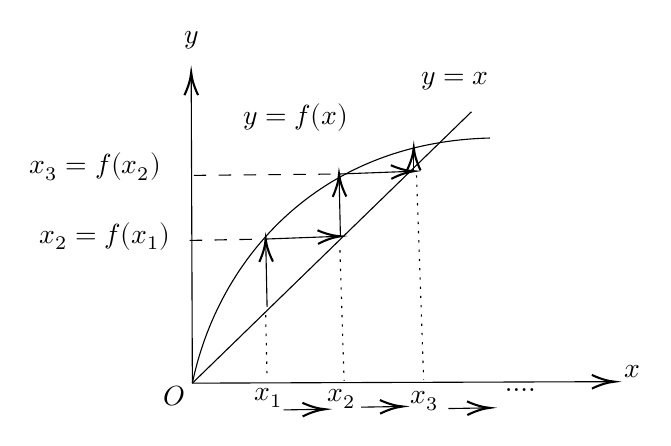
\begin{tikzpicture}[x=0.75pt,y=0.75pt,yscale=-1,xscale=1]
                            \draw    (78,180) -- (279.43,179.29) ;
                            \draw [shift={(281.43,179.29)}, rotate = 179.8] [color={rgb, 255:red, 0; green, 0; blue, 0 }  ][line width=0.75]    (10.93,-3.29) .. controls (6.95,-1.4) and (3.31,-0.3) .. (0,0) .. controls (3.31,0.3) and (6.95,1.4) .. (10.93,3.29)   ;
                            \draw    (78,180) -- (77.44,32.29) ;
                            \draw [shift={(77.43,30.29)}, rotate = 89.78] [color={rgb, 255:red, 0; green, 0; blue, 0 }  ][line width=0.75]    (10.93,-3.29) .. controls (6.95,-1.4) and (3.31,-0.3) .. (0,0) .. controls (3.31,0.3) and (6.95,1.4) .. (10.93,3.29)   ;
                            \draw    (78,180) -- (212.43,49.29) ;
                            \draw    (78,180) .. controls (90,121.9) and (137.33,63.9) .. (221.33,61.9) ;
                            \draw  [dash pattern={on 0.84pt off 2.51pt}]  (113.33,147.24) -- (114,177.9) ;
                            \draw  [dash pattern={on 0.84pt off 2.51pt}]  (186,79.9) -- (189.43,178.29) ;
                            \draw  [dash pattern={on 0.84pt off 2.51pt}]  (149.1,115.95) -- (151.1,178.95) ;
                            \draw    (122,192.9) -- (140,192.6) ;
                            \draw [shift={(142,192.57)}, rotate = 179.05] [color={rgb, 255:red, 0; green, 0; blue, 0 }  ][line width=0.75]    (10.93,-3.29) .. controls (6.95,-1.4) and (3.31,-0.3) .. (0,0) .. controls (3.31,0.3) and (6.95,1.4) .. (10.93,3.29)   ;
                            \draw    (159.33,191.57) -- (177.33,191.27) ;
                            \draw [shift={(179.33,191.24)}, rotate = 179.05] [color={rgb, 255:red, 0; green, 0; blue, 0 }  ][line width=0.75]    (10.93,-3.29) .. controls (6.95,-1.4) and (3.31,-0.3) .. (0,0) .. controls (3.31,0.3) and (6.95,1.4) .. (10.93,3.29)   ;
                            \draw    (201.33,192.24) -- (219.33,191.94) ;
                            \draw [shift={(221.33,191.9)}, rotate = 179.05] [color={rgb, 255:red, 0; green, 0; blue, 0 }  ][line width=0.75]    (10.93,-3.29) .. controls (6.95,-1.4) and (3.31,-0.3) .. (0,0) .. controls (3.31,0.3) and (6.95,1.4) .. (10.93,3.29)   ;
                            \draw    (114,143.24) -- (113.37,112.57) ;
                            \draw [shift={(113.33,110.57)}, rotate = 88.83] [color={rgb, 255:red, 0; green, 0; blue, 0 }  ][line width=0.75]    (10.93,-3.29) .. controls (6.95,-1.4) and (3.31,-0.3) .. (0,0) .. controls (3.31,0.3) and (6.95,1.4) .. (10.93,3.29)   ;
                            \draw    (113.33,110.57) -- (147.33,109.31) ;
                            \draw [shift={(149.33,109.24)}, rotate = 177.88] [color={rgb, 255:red, 0; green, 0; blue, 0 }  ][line width=0.75]    (10.93,-3.29) .. controls (6.95,-1.4) and (3.31,-0.3) .. (0,0) .. controls (3.31,0.3) and (6.95,1.4) .. (10.93,3.29)   ;
                            \draw    (149.33,109.24) -- (148.71,81.24) ;
                            \draw [shift={(148.67,79.24)}, rotate = 88.73] [color={rgb, 255:red, 0; green, 0; blue, 0 }  ][line width=0.75]    (10.93,-3.29) .. controls (6.95,-1.4) and (3.31,-0.3) .. (0,0) .. controls (3.31,0.3) and (6.95,1.4) .. (10.93,3.29)   ;
                            \draw    (148.67,79.24) -- (182.67,77.98) ;
                            \draw [shift={(184.67,77.9)}, rotate = 177.88] [color={rgb, 255:red, 0; green, 0; blue, 0 }  ][line width=0.75]    (10.93,-3.29) .. controls (6.95,-1.4) and (3.31,-0.3) .. (0,0) .. controls (3.31,0.3) and (6.95,1.4) .. (10.93,3.29)   ;
                            \draw    (184.67,77.9) -- (184.67,68.57) ;
                            \draw [shift={(184.67,66.57)}, rotate = 90] [color={rgb, 255:red, 0; green, 0; blue, 0 }  ][line width=0.75]    (10.93,-3.29) .. controls (6.95,-1.4) and (3.31,-0.3) .. (0,0) .. controls (3.31,0.3) and (6.95,1.4) .. (10.93,3.29)   ;
                            \draw  [dash pattern={on 4.5pt off 4.5pt}]  (76.67,111.24) -- (113.33,110.57) ;
                            \draw  [dash pattern={on 4.5pt off 4.5pt}]  (78.67,79.9) -- (148.67,79.24) ;
                            \draw (63,180) node [anchor=north west][inner sep=0.75pt]   [align=left] {$\displaystyle O$};
                            \draw (73,9) node [anchor=north west][inner sep=0.75pt]   [align=left] {$\displaystyle y$};
                            \draw (285,170) node [anchor=north west][inner sep=0.75pt]   [align=left] {$\displaystyle x$};
                            \draw (187,29) node [anchor=north west][inner sep=0.75pt]   [align=left] {$\displaystyle y=x$};
                            \draw (106.67,181.24) node [anchor=north west][inner sep=0.75pt]   [align=left] {$\displaystyle x_{1}$};
                            \draw (142,181.9) node [anchor=north west][inner sep=0.75pt]   [align=left] {$\displaystyle x_{2}$};
                            \draw (181.71,182.64) node [anchor=north west][inner sep=0.75pt]   [align=left] {$\displaystyle x_{3}$};
                            \draw (35.95,101.24) node [anchor=north] [inner sep=0.75pt]  [font=\normalsize] [align=left] {$\displaystyle {\textstyle x_{2} =f( x_{1})}$};
                            \draw (31.28,67.9) node [anchor=north] [inner sep=0.75pt]  [font=\normalsize] [align=left] {$\displaystyle {\textstyle x_{3} =f( x_{2})}$};
                            \draw (101.33,44.3) node [anchor=north west][inner sep=0.75pt]    {$y=f( x)$};
                            \draw (227.33,181.24) node [anchor=north west][inner sep=0.75pt]   [align=left] {....};
                            \end{tikzpicture}
                        \end{center}
                        若$f(x)$单调增加,且$x_1>x_2$,则数列单增的图像是这样的
                        \begin{center}
                            \tikzset{every picture/.style={line width=0.75pt}} %set default line width to 0.75pt        
                            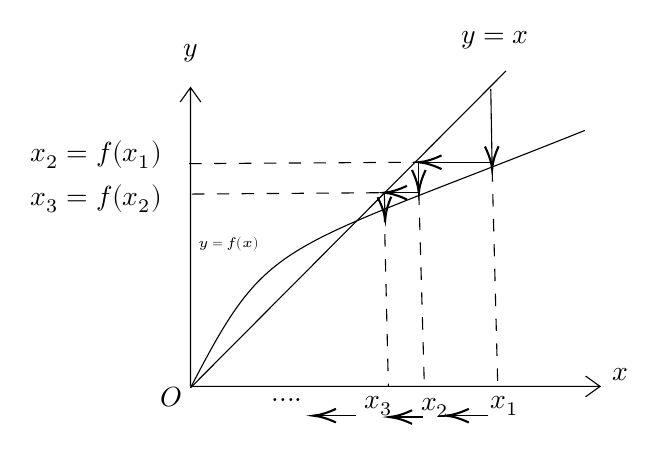
\begin{tikzpicture}[x=0.75pt,y=0.75pt,yscale=-1,xscale=1]
                            \draw  (138.86,238.57) -- (336.19,238.57)(138.86,94.57) -- (138.86,238.57) -- cycle (329.19,233.57) -- (336.19,238.57) -- (329.19,243.57) (133.86,101.57) -- (138.86,94.57) -- (143.86,101.57)  ;
                            \draw    (138.86,239.24) -- (290.86,86.57) ;
                            \draw    (138.86,239.24) .. controls (176.86,165.9) and (178.86,175.24) .. (328.86,115.24) ;
                            \draw  [dash pattern={on 4.5pt off 4.5pt}]  (248.86,145.24) -- (251.52,238.57) ;
                            \draw    (248.86,130.57) -- (248.86,143.24) ;
                            \draw [shift={(248.86,145.24)}, rotate = 270] [color={rgb, 255:red, 0; green, 0; blue, 0 }  ][line width=0.75]    (10.93,-3.29) .. controls (6.95,-1.4) and (3.31,-0.3) .. (0,0) .. controls (3.31,0.3) and (6.95,1.4) .. (10.93,3.29)   ;
                            \draw    (284.19,130.57) -- (250.86,130.57) ;
                            \draw [shift={(248.86,130.57)}, rotate = 360] [color={rgb, 255:red, 0; green, 0; blue, 0 }  ][line width=0.75]    (10.93,-3.29) .. controls (6.95,-1.4) and (3.31,-0.3) .. (0,0) .. controls (3.31,0.3) and (6.95,1.4) .. (10.93,3.29)   ;
                            \draw    (283.52,95.24) -- (284.16,131.91) ;
                            \draw [shift={(284.19,133.9)}, rotate = 269.01] [color={rgb, 255:red, 0; green, 0; blue, 0 }  ][line width=0.75]    (10.93,-3.29) .. controls (6.95,-1.4) and (3.31,-0.3) .. (0,0) .. controls (3.31,0.3) and (6.95,1.4) .. (10.93,3.29)   ;
                            \draw    (248.86,145.24) -- (234.19,145.24) ;
                            \draw [shift={(232.19,145.24)}, rotate = 360] [color={rgb, 255:red, 0; green, 0; blue, 0 }  ][line width=0.75]    (10.93,-3.29) .. controls (6.95,-1.4) and (3.31,-0.3) .. (0,0) .. controls (3.31,0.3) and (6.95,1.4) .. (10.93,3.29)   ;
                            \draw    (232.19,145.24) -- (232.59,156.24) ;
                            \draw [shift={(232.67,158.24)}, rotate = 267.9] [color={rgb, 255:red, 0; green, 0; blue, 0 }  ][line width=0.75]    (10.93,-3.29) .. controls (6.95,-1.4) and (3.31,-0.3) .. (0,0) .. controls (3.31,0.3) and (6.95,1.4) .. (10.93,3.29)   ;
                            \draw  [dash pattern={on 4.5pt off 4.5pt}]  (232.19,153.24) -- (234.19,238.57) ;
                            \draw  [dash pattern={on 4.5pt off 4.5pt}]  (284.19,133.9) -- (286.86,237.24) ;
                            \draw  [dash pattern={on 4.5pt off 4.5pt}]  (139.52,145.9) -- (232.19,145.24) ;
                            \draw  [dash pattern={on 4.5pt off 4.5pt}]  (138.19,131.24) -- (248.86,130.57) ;
                            \draw    (282.38,252.67) -- (264,252.67) ;
                            \draw [shift={(262,252.67)}, rotate = 360] [color={rgb, 255:red, 0; green, 0; blue, 0 }  ][line width=0.75]    (10.93,-3.29) .. controls (6.95,-1.4) and (3.31,-0.3) .. (0,0) .. controls (3.31,0.3) and (6.95,1.4) .. (10.93,3.29)   ;
                            \draw    (251.05,253.33) -- (236.67,253.33) ;
                            \draw [shift={(234.67,253.33)}, rotate = 360] [color={rgb, 255:red, 0; green, 0; blue, 0 }  ][line width=0.75]    (10.93,-3.29) .. controls (6.95,-1.4) and (3.31,-0.3) .. (0,0) .. controls (3.31,0.3) and (6.95,1.4) .. (10.93,3.29)   ;
                            \draw    (218.38,252.67) -- (200,252.67) ;
                            \draw [shift={(198,252.67)}, rotate = 360] [color={rgb, 255:red, 0; green, 0; blue, 0 }  ][line width=0.75]    (10.93,-3.29) .. controls (6.95,-1.4) and (3.31,-0.3) .. (0,0) .. controls (3.31,0.3) and (6.95,1.4) .. (10.93,3.29)   ;
                            \draw (123.33,237.57) node [anchor=north west][inner sep=0.75pt]   [align=left] {$\displaystyle O$};
                            \draw (134,72.57) node [anchor=north west][inner sep=0.75pt]   [align=left] {$\displaystyle y$};
                            \draw (340.67,228.57) node [anchor=north west][inner sep=0.75pt]   [align=left] {$\displaystyle x$};
                            \draw (141.33,165.57) node [anchor=north west][inner sep=0.75pt]  [font=\tiny] [align=left] {$\displaystyle y=f( x)$};
                            \draw (60.67,140.24) node [anchor=north west][inner sep=0.75pt]   [align=left] {$\displaystyle x_{3} =f( x_{2})$};
                            \draw (60.67,118.9) node [anchor=north west][inner sep=0.75pt]   [align=left] {$\displaystyle x_{2} =f( x_{1})$};
                            \draw (282,242.24) node [anchor=north west][inner sep=0.75pt]   [align=left] {$\displaystyle x_{1}$};
                            \draw (248.67,242.9) node [anchor=north west][inner sep=0.75pt]   [align=left] {$\displaystyle x_{2}$};
                            \draw (221.33,242.24) node [anchor=north west][inner sep=0.75pt]   [align=left] {$\displaystyle x_{3}$};
                            \draw (176.67,243.33) node [anchor=north west][inner sep=0.75pt]   [align=left] {$\displaystyle ....$};
                            \draw (268,66) node [anchor=north west][inner sep=0.75pt]   [align=left] {$\displaystyle y=x$};
                            \end{tikzpicture}
                        \end{center}
                    \end{proof}
                    \item 若$f^{\prime}(x)<0$,$x\in $区间$I$, 则数列$\{x_n\}$ 不单调
                    \begin{proof}
                        若$f(x)$单调递减,且$x_1<x_2$时,则图像为
                        \begin{center}
                            \tikzset{every picture/.style={line width=0.75pt}} %set default line width to 0.75pt        
                            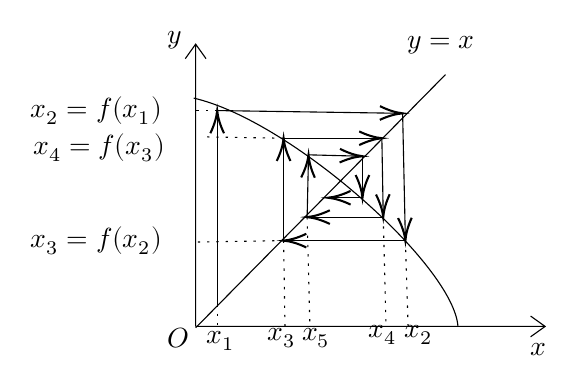
\begin{tikzpicture}[x=0.75pt,y=0.75pt,yscale=-1,xscale=1]
                            \draw  (125.33,214.67) -- (293.71,214.67)(125.33,78.67) -- (125.33,214.67) -- cycle (286.71,209.67) -- (293.71,214.67) -- (286.71,219.67) (120.33,85.67) -- (125.33,78.67) -- (130.33,85.67)  ;
                            \draw    (125.33,215.33) -- (245.71,93.33) ;
                            \draw    (124.38,104.67) .. controls (171.05,115.33) and (249.71,185.33) .. (251.71,214.67) ;
                            \draw    (135.71,204) -- (135.71,112.67) ;
                            \draw [shift={(135.71,110.67)}, rotate = 90] [color={rgb, 255:red, 0; green, 0; blue, 0 }  ][line width=0.75]    (10.93,-3.29) .. controls (6.95,-1.4) and (3.31,-0.3) .. (0,0) .. controls (3.31,0.3) and (6.95,1.4) .. (10.93,3.29)   ;
                            \draw  [dash pattern={on 0.84pt off 2.51pt}]  (135.71,204) -- (135.71,216) ;
                            \draw    (135.71,110.67) -- (223.05,111.97) ;
                            \draw [shift={(225.05,112)}, rotate = 180.86] [color={rgb, 255:red, 0; green, 0; blue, 0 }  ][line width=0.75]    (10.93,-3.29) .. controls (6.95,-1.4) and (3.31,-0.3) .. (0,0) .. controls (3.31,0.3) and (6.95,1.4) .. (10.93,3.29)   ;
                            \draw    (225.05,112) -- (226.34,171.33) ;
                            \draw [shift={(226.38,173.33)}, rotate = 268.75] [color={rgb, 255:red, 0; green, 0; blue, 0 }  ][line width=0.75]    (10.93,-3.29) .. controls (6.95,-1.4) and (3.31,-0.3) .. (0,0) .. controls (3.31,0.3) and (6.95,1.4) .. (10.93,3.29)   ;
                            \draw    (226.38,173.33) -- (169.71,173.33) ;
                            \draw [shift={(167.71,173.33)}, rotate = 360] [color={rgb, 255:red, 0; green, 0; blue, 0 }  ][line width=0.75]    (10.93,-3.29) .. controls (6.95,-1.4) and (3.31,-0.3) .. (0,0) .. controls (3.31,0.3) and (6.95,1.4) .. (10.93,3.29)   ;
                            \draw    (167.71,173.33) -- (167.71,126) ;
                            \draw [shift={(167.71,124)}, rotate = 90] [color={rgb, 255:red, 0; green, 0; blue, 0 }  ][line width=0.75]    (10.93,-3.29) .. controls (6.95,-1.4) and (3.31,-0.3) .. (0,0) .. controls (3.31,0.3) and (6.95,1.4) .. (10.93,3.29)   ;
                            \draw    (167.71,124) -- (213.05,124) ;
                            \draw [shift={(215.05,124)}, rotate = 180] [color={rgb, 255:red, 0; green, 0; blue, 0 }  ][line width=0.75]    (10.93,-3.29) .. controls (6.95,-1.4) and (3.31,-0.3) .. (0,0) .. controls (3.31,0.3) and (6.95,1.4) .. (10.93,3.29)   ;
                            \draw    (215.05,124) -- (215.68,160) ;
                            \draw [shift={(215.71,162)}, rotate = 268.99] [color={rgb, 255:red, 0; green, 0; blue, 0 }  ][line width=0.75]    (10.93,-3.29) .. controls (6.95,-1.4) and (3.31,-0.3) .. (0,0) .. controls (3.31,0.3) and (6.95,1.4) .. (10.93,3.29)   ;
                            \draw    (215.71,162) -- (181.05,162) ;
                            \draw [shift={(179.05,162)}, rotate = 360] [color={rgb, 255:red, 0; green, 0; blue, 0 }  ][line width=0.75]    (10.93,-3.29) .. controls (6.95,-1.4) and (3.31,-0.3) .. (0,0) .. controls (3.31,0.3) and (6.95,1.4) .. (10.93,3.29)   ;
                            \draw    (179.05,162) -- (179.67,134) ;
                            \draw [shift={(179.71,132)}, rotate = 91.27] [color={rgb, 255:red, 0; green, 0; blue, 0 }  ][line width=0.75]    (10.93,-3.29) .. controls (6.95,-1.4) and (3.31,-0.3) .. (0,0) .. controls (3.31,0.3) and (6.95,1.4) .. (10.93,3.29)   ;
                            \draw    (179.71,132) -- (203.71,132.62) ;
                            \draw [shift={(205.71,132.67)}, rotate = 181.47] [color={rgb, 255:red, 0; green, 0; blue, 0 }  ][line width=0.75]    (10.93,-3.29) .. controls (6.95,-1.4) and (3.31,-0.3) .. (0,0) .. controls (3.31,0.3) and (6.95,1.4) .. (10.93,3.29)   ;
                            \draw    (205.71,132.67) -- (205.71,150.67) ;
                            \draw [shift={(205.71,152.67)}, rotate = 270] [color={rgb, 255:red, 0; green, 0; blue, 0 }  ][line width=0.75]    (10.93,-3.29) .. controls (6.95,-1.4) and (3.31,-0.3) .. (0,0) .. controls (3.31,0.3) and (6.95,1.4) .. (10.93,3.29)   ;
                            \draw  [dash pattern={on 0.84pt off 2.51pt}]  (167.71,173.33) -- (168.38,215.33) ;
                            \draw  [dash pattern={on 0.84pt off 2.51pt}]  (179.05,162) -- (180.38,214.67) ;
                            \draw  [dash pattern={on 0.84pt off 2.51pt}]  (215.71,162) -- (217.05,214) ;
                            \draw  [dash pattern={on 0.84pt off 2.51pt}]  (226.38,173.33) -- (227.71,215.33) ;
                            \draw    (205.71,152.67) -- (191.05,152.67) ;
                            \draw [shift={(189.05,152.67)}, rotate = 360] [color={rgb, 255:red, 0; green, 0; blue, 0 }  ][line width=0.75]    (10.93,-3.29) .. controls (6.95,-1.4) and (3.31,-0.3) .. (0,0) .. controls (3.31,0.3) and (6.95,1.4) .. (10.93,3.29)   ;
                            \draw  [dash pattern={on 0.84pt off 2.51pt}]  (135.71,110.67) -- (123.71,110.67) ;
                            \draw  [dash pattern={on 0.84pt off 2.51pt}]  (167.71,124) -- (128.71,123.33) ;
                            \draw  [dash pattern={on 0.84pt off 2.51pt}]  (167.71,173.33) -- (126.38,174) ;
                            \draw (110.67,214) node [anchor=north west][inner sep=0.75pt]   [align=left] {$\displaystyle O$};
                            \draw (129.33,215.67) node [anchor=north west][inner sep=0.75pt]   [align=left] {$\displaystyle x_{1}$};
                            \draw (224.67,213) node [anchor=north west][inner sep=0.75pt]   [align=left] {$\displaystyle x_{2}$};
                            \draw (158.67,214.33) node [anchor=north west][inner sep=0.75pt]   [align=left] {$\displaystyle x_{3}$};
                            \draw (175.33,214.33) node [anchor=north west][inner sep=0.75pt]   [align=left] {$\displaystyle x_{5}$};
                            \draw (207.33,213) node [anchor=north west][inner sep=0.75pt]   [align=left] {$\displaystyle x_{4}$};
                            \draw (226,73.67) node [anchor=north west][inner sep=0.75pt]   [align=left] {$\displaystyle y=x$};
                            \draw (285.33,221.33) node [anchor=north west][inner sep=0.75pt]   [align=left] {$\displaystyle x$};
                            \draw (110.67,71) node [anchor=north west][inner sep=0.75pt]   [align=left] {$\displaystyle y$};
                            \draw (44.67,165.33) node [anchor=north west][inner sep=0.75pt]   [align=left] {$\displaystyle x_{3} =f( x_{2})$};
                            \draw (46,120.67) node [anchor=north west][inner sep=0.75pt]   [align=left] {$\displaystyle x_{4} =f( x_{3})$};
                            \draw (44.67,102.67) node [anchor=north west][inner sep=0.75pt]   [align=left] {$\displaystyle x_{2} =f( x_{1})$};
                            \end{tikzpicture}
                        \end{center}
                    \end{proof}
                \end{itemize}
            \end{enumerate}
        \item 利用压缩映射(先斩后奏):先令$\lim_{n\to\infty} x_n=A$,然后等式$x_{n+1}=f(x_n)$两端取极限解得$A$,得到极限初步结果,最后再证明$\lim_{n\to\infty} x_n=A$.\textcolor{red}{核心是用$x_n=f(x_{n-1})$证明一个递推不等式$|x_n-a| \leqslant A|x_{n-1}-a|$,其中$0<A<1$}
    \end{enumerate}
    \begin{problem}
        设$0<x_1<3,x_{n+1}=\sqrt{x_n\left(3-x_n\right)}\left(n=1,2,...\right)$,证明:数列$x_n$极限存在并求此极限
    \end{problem}
    \begin{solution}
        由$0<x_1<3,x_{n+1}=\sqrt{x_n(3-x_n)}$可得:
        $$
            x_{n+1}=\sqrt{x_n(3-x_n)}\leqslant \dfrac{3}{2}
        $$
        可知数列$x_n$存在上界,令$x_{n+1}-x_n$可得:
        \begin{align*}
            x_{n+1}-x_n & = \sqrt{x_n(3-x_n)}-x_n \\
          & = \dfrac{x_n(3-x_n)-x_n^2}{\sqrt{x_n(3-x_n)}+x_n}\\ 
          & = \dfrac{x_n(3-2x_n)}{\sqrt{x_n(3-x_n)}+x_n}\geqslant0
        \end{align*}
        故$x_n$单调递增,根据数列单调有界定理,该数列极限存在,因此设$\lim_{x_n}=a$,对等式$x_{n+1}=\sqrt{x_n(3-x_n)}$左右两边取极限得:$a=\sqrt{a(3-a)}$.解得$a=\dfrac{3}{2}$\\综上,数列极限为$\dfrac{3}{2}$
    \end{solution}
    \begin{note}
        出现本题的形式$x_{n+1}=\sqrt{x_n(3-x_n)}$可以使用常用不等式\ref{cybds1},对不等式放缩计算极限.
    \end{note}
    \begin{problem}
        设$x_1=\sqrt{6},x_2=\sqrt{6+\sqrt{6}},\cdotp\cdotp\cdotp,x_n=\sqrt{6+\sqrt{6+\sqrt{6+\cdots+\sqrt{6}}}}$,求极限$\lim_{n \to \infty}x_n$
    \end{problem}
    \begin{solution}
        由题意可知,讲数列的表达式可抽象为$x_{n+1}=\sqrt{6+x_n}$,其函数表达式为$f(x)=\sqrt{6+x}$,对其求导可得:$f'(x)=\dfrac{1}{2\sqrt{6+x}}>0$,由于$x_1<x_2$因此数列单调递增.又因为$x_1=\sqrt{6}<3$,若$x_n<3$,则$x_{n+1}=\sqrt{6+x_n}<3$,从而$x_n<3$,即数列$x_n$有上界,则$\lim_{n\to \infty} x_n$存在,设$\lim_{n\to \infty}x_n=a$,由于$0<x_n<3$,故由极限的保序性可得:$0\leqslant a \leqslant 3$.$x_{n+1}=\sqrt{6+x_n}$,两侧取极限得:$a=\sqrt{6+a}$,解得a=3,综上数列极限为$\lim_{n\to \infty }x_n=3$
    \end{solution}
    \begin{note}
        除此之外,本题还可以使用压缩映射进行求解:
        \begin{solution}
            直接证明$\lim_{n\to \infty}x_n=3$,由$x_{n+1}=\sqrt{6+x_n}$知:\begin{align*}
              \text{原式} & =|x_n-3|=|\sqrt{6+x_{n-1}}-3|
            \end{align*}
            对于此处的运算,我们可以使用拉格朗日中值定理进行化简,即
            \begin{align*}
              \text{原式} & =|\sqrt{6+x_{n-1}}-3| \\
              & = |\sqrt{6+x_{n-1}}-\sqrt{9}|\\
              & = \dfrac{1}{2\sqrt{\varepsilon}}|x_{n-1}-3|<\dfrac{1}{2}|x_{n-1}-3|<\dfrac{1}{2^2}|x_{n-2}-3|<...<\dfrac{1}{2^{n-1}}|x_1-3|\to 0 \quad (n\to \infty)
            \end{align*}
            则$\lim_{n\to \infty}x_n=3$\\
            当然也可以使用有理化进行化简:
            \begin{align*}
              \text{原式} & =\dfrac{|x_{n-1}-3|}{\sqrt{6+x_{n-1}}+3}<\frac{1}{3}\mid x_{n-1}-3\mid<\frac{1}{3^{2}}\mid x_{n-2}-3\mid<\cdots<\frac{1}{3^{n-1}}\mid x_{1}-3\mid\to0 \quad (n\to \infty)
            \end{align*}
            综上
            $$
                0 \leqslant \lim_{n\to \infty}|x_n-3| \leqslant \lim_{n\to \infty} \dfrac{1}{3^{n-1}}|x_1-3|
            $$使用夹逼准则可以得到$\lim_{n\to \infty}x_n=3$
        \end{solution}
    \end{note}
    \begin{problem}
        设$x_1=2,x_{n+1}=2+\dfrac1{x_n}(n=1,2,...)$,求极限$\lim_{n\to\infty}x_n$
    \end{problem}
    \begin{solution}
        令 $f(x)=2+\dfrac1x$,则 $x_{n+1}=f(x_n)$,显然 $f(x)$ 在$(0,+\infty)$上单调减,故$\{x_n\}$不具有单调性,因此只能使用压缩映射.\\
        令$\lim_{n\to \infty}x_n=a$,则$\lim_{n \to \infty}x_{n+1}=2+\dfrac{1}{\lim_{n\to \infty}x_n} \Rightarrow a=2+\dfrac{1}{a}$,解得$a=1\pm \sqrt{2}$.\\
        由题设知$x_n\geq2$,故由极限的保号性知,$a\geq2$,从而$a=1 \pm \sqrt{2}$,以下证明$\lim_{n\to \infty}x_n=1+\sqrt{2}$\\
        $\mid x_n-a\mid=\left|\left(2+\dfrac{1}{x_{n-1}}\right)-\left(2+\dfrac{1}{a}\right)\right|=\left|\dfrac{x_{n-1}-a}{ax_{n-1}}\right|\leqslant\dfrac{\left|x_{n-1}-a\right|}{2a}\leqslant\dfrac{\left|x_{n-1}-a\right|}{2} \leqslant \dfrac{\mid x_{n-2}-a\mid}{2^2} \leqslant \cdots \leqslant \dfrac{\mid x_1-a\mid}{2^{n-1}}\to0$
    \end{solution}
    \begin{note}
        \textcolor{red}{需要切记的是在压缩映射中,极限值为根式时,要用极限时的等式对极限值进行替换},比如在本题中在证明数列极限为$1+\pm \sqrt{2}$中,应写为$|x_n -a|$,而不是$|x_n -1 -\sqrt{2}|$
    \end{note}
    \begin{problem}
        \uline{设$x_1=\sqrt{a}(a>0),x_{n+1}=\sqrt{a+x_n}$,证明:$\lim_{n\to\infty} x_n$ 存在,并求其值.}
    \end{problem}
        本题有四种方法,下面依次给出求解:
        \begin{solution}{\textbf{法1:数学归纳法找上界:}}
            数列形式可写为$f(x)=\sqrt{a+x}$,则$f'(x)=\dfrac{1}{2\sqrt{a+x}}>0$,因此$f(x)$单增,又$x_1=\sqrt{a},x_2=\sqrt{a+\sqrt{a}},x_2>x_1$,因此$x_n$单增.\\
            假设$\lim_{n\to \infty}x_n=A=\dfrac{1+\sqrt{1+4a}}{2}$.由第一数学归纳法可得:\\
            验证$x_1=\sqrt{a}<\dfrac{1+\sqrt{1+4a}}{2}$,即证:$$
                2\sqrt{a}<1+\sqrt{1+4a}
            $$
            $$
                4a<2+4a+2\sqrt{1+4a}
            $$
            假设$x_n<\dfrac{1+\sqrt{1+4a}}{2}$成立,验证$x_{n+1}<\dfrac{1+\sqrt{1+4a}}{2}$
            即证:$$
                2\sqrt{a+x_n}<1+\sqrt{1+4a}
            $$
            $$
                4a+4x_n<2+4a+2\sqrt{1+4a}
            $$
            $$
                4x_n<2+2\sqrt{1+4a}
            $$
            即证:$x_n <\dfrac{1+\sqrt{1+4a}}{2}$,显然成立.\\
            综上:$x_n < \dfrac{1+\sqrt{1+4a}}{2}$,且$x_n$单增,那么$\lim_{n\to \infty}x_n$存在,令$\lim_{n\to \infty}x_n=A$,则$A=\sqrt{a+A}$,解得$A=\dfrac{1+\sqrt{1+4a}}{2}$\\
            综上$\lim_{n\to \infty}x_n=\dfrac{1+\sqrt{1+4a}}{2}$
        \end{solution}
        \begin{solution}{\textbf{法2:对方法一进行化简(最佳):}}
            数列形式可写为$f(x)=\sqrt{a+x}$,则$f'(x)=\dfrac{1}{2\sqrt{a+x}}>0$,因此$f(x)$单增,又$x_1=\sqrt{a},x_2=\sqrt{a+\sqrt{a}},x_2>x_1$,因此$x_n$单增.\\
            设$A=\sqrt{a+A}$ 假设$\lim_{n\to \infty}x_n=A=\dfrac{1+\sqrt{1+4a}}{2}$.由第一数学归纳法可得:\\
            验证$x_1<A$,即证:$$
                x_1=\sqrt{a},A=\sqrt{a+A}
            $$
            $$
                \sqrt{a}<\sqrt{a+A} \Rightarrow x_1 <A
            $$
            假设$x_n<A$成立,验证$x_{n+1} < A $
            即证:$$
                x_{n+1}=\sqrt{x+x_n}<\sqrt{a+A}=A
            $$
            即证:$x_n < A$,显然成立.\\
            综上:$x_n < A$,且$x_n$单增,那么$\lim_{n\to \infty}x_n$存在,令$\lim_{n\to \infty}x_n=M$,则$M=\sqrt{a+M}$,解得$M=\dfrac{1+\sqrt{1+4a}}{2}$
        \end{solution}
        \begin{solution}{\textbf{法3:构造不等式进行放缩\footnote{其实不好放缩,但是可以硬往条件上凑}}}
            易知$x_n$,单调递增,且$x_n>0 \Rightarrow \begin{cases}
                x_{n+1}>x_n>...>x_1=\sqrt{a}\\
                \dfrac{x_n}{x_{n+1}}<1
            \end{cases}$
        \begin{align*}
          x_{n+1} & = \sqrt{a+x_n} \\
          & \Rightarrow x^2_{n+1}=a+x_n\\
          & \Rightarrow \dfrac{a}{x_{n+1}}+\dfrac{x_n}{x_{n+1}}\\
          & \Rightarrow x_{n+1}<\dfrac{a}{x_{n+1}}+1
        \end{align*}
        $x_n$单增且有上界,因此$\lim_{n\to \infty}x_n$存在.
        设$\lim_{n\to \infty}x_n=A$,则$A=\sqrt{a+A}$,解得$A=\dfrac{1+\sqrt{1+4a}}{2}$\\
        综上$\lim_{n\to \infty}x_n=\dfrac{1+\sqrt{1+4a}}{2}$
        \end{solution}
        \begin{solution}{\textbf{法4:压缩映射+有理化}}
            \begin{align*}
              |x_n -A| & = |\sqrt{a+x_{n+1}}-\sqrt{a+A}|\\
              & = \dfrac{|x_{n-1}-A|}{\sqrt{a+x_{n-1}}+\sqrt{a+A}} \leqslant \dfrac{1}{2\sqrt{a}}|x_{n+1}-A|
            \end{align*}
        \end{solution}
    \begin{problem}
        \uline{设数列$\{x_n\}$ 满足$:x_1>0,x_ne^{x_{n+1}}=e^{x_n}-1(n=1,2,\cdots)$.证明$\{x_n\}$收敛,并求$\lim_{n\to\infty} x_n$ }    
    \end{problem}
    \begin{solution}
        $$ 
           x_{n+1} - x_{n} = \ln\biggl(\frac{\mathrm{e}^{x_{n}} - 1}{x_{n}}\biggr)- x_{n} = \ln\biggl(\frac{\mathrm{e}^{x_{n}} - 1}{x_{n}\mathrm{e}^{x_{n}}}\biggr).
        $$
        令$f(x)=e^x-1-xe^x$,则$f'(x)=-xe^x$.当$x>0$时,$f(x)$ 在$[0,+\infty)$ 上单调减少,于是,$f(x)<f\left(0\right)=0.$从而,当$x>0$ 时
        $$
            \dfrac{\mathrm{e}^x-1}{x\mathrm{e}^x}-1 = \dfrac{\mathrm{e}^x-1-x\mathrm{e}^x}{x\mathrm{e}^x}<0
        $$即$\dfrac{e^x-1}{xe^x}<1$
        又因为对所有的正整数$n$,都有$x_n>0$,所以$\ln\left(\dfrac{\mathrm{e}^{x_n}-1}{x_n\mathrm{e}^{x_n}}\right)<\ln1=0$,即$x_{n+1}-x_n<0.$ 因此,数列$|x_n|$单调减少.\\
        由单调有界准则可知,数列$|x_n|$收敛.由于对所有的正整数$n$,都有$x_n>0$,故$\lim_{n\to\infty}x_n=a\geqslant0.$\\
        对$x_n\mathrm{e}^{x_n+1}=\mathrm{e}^{x_n}-1$ 两端同时令$n\to\infty$,可得$a\mathrm{e}^n=\mathrm{e}^a-1$,由前面的结果可知,$x=0$ 是$f(x)=e^x-1-xe^x$ 在$[0,+\infty)$上的唯一零点,因此,$a=0$,即$\lim_{n\to \infty}x_n=0.$
    \end{solution}
    %  ############################ 正文部分
    \ifx\allfiles\undefined
\end{sloppypar}
\end{document}
\fi
 